%\documentclass[german,reviews,examples]{isasthesis}
% \documentclass[english,reviews,examples]{isasthesis}
\documentclass[english]{isasthesis}
\usepackage[utf8]{inputenc}

%%%%%%%%%%%%%%%%%%%%%%%%%%%%%%%%%%
% Edit notation.tex if necessary
%%%%%%%%%%%%%%%%%%%%%%%%%%%%%%%%%%

%%%%%%%%%%%%%%%%%%%%%%%%
% Document properties
%%%%%%%%%%%%%%%%%%%%%%%%

\title{Comparison of Newton-Flow Particle Filters and Classical
	Particle Filters in High-Dimensional Nonlinear Systems}
\author{Yiqing Wang}
\date{April 2026}

\thesistype{Master Thesis}
\firstsupervisor{Prof. Dr.-Ing. Uwe D. Hanebeck}
\secondsupervisor{Dr. Daniel Frisch}

%%%%%%%%%%%%%%%%%%%%%%%%
% Document
%%%%%%%%%%%%%%%%%%%%%%%%
\clubpenalty = 100000
\brokenpenalty = 100000
\finalhyphendemerits = 100000
\displaywidowpenalty = 1000000
\widowpenalty = 1000000
\usepackage{makecell}
\usepackage{bm}
\usepackage{listings}
\usepackage[nameinlink]{cleveref}
\usepackage{acro}
\DeclareAcronym{nff}{short = NFF, long = Newton-Flow Filter}
\DeclareAcronym{pf}{short = PF, long = Traditional Particle Filter}
\DeclareAcronym{gpf}{short = GPF, long = Gaussian Particle Filter}
\DeclareAcronym{dmd}{short = DMD, long = Dirac Mixture Density}
\DeclareAcronym{lcd}{short = LCD, long = Localized Cumulative Distribution}
\DeclareAcronym{cvm}{short = CVM, long = Cramér--von Mises}
\DeclareAcronym{ode}{short = ODE, long = Ordinary Differential Equation}
\DeclareAcronym{sde}{short = SDE, long = Stochastic Differential Equation}
\DeclareAcronym{minres}{short = MINRES, long = Minimum Residual Method}
\DeclareAcronym{vcabm}{short = VCABM, long = Variable-Coefficient Adams--Bashforth--Moulton}
\DeclareAcronym{rmse}{short = RMSE, long = Root Mean Square Error}
\DeclareAcronym{gae}{short = GAE, long = Geometric Average Error}
\DeclareAcronym{rfe}{short = RFE, long = Relative Frobenius Error}
\DeclareAcronym{merf}{short = MERF, long = Measurement Error Reduction Factor}
\DeclareAcronym{anees}{short = ANEES, long = Average Normalized Estimation Error Squared}
\begin{document}
	\maketitle
	
	\begin{abstract}
		This thesis compares the performance of the \ac{nff}, the \ac{pf}, and the \ac{gpf} in high-dimensional nonlinear systems.
		
		First, a matrix-free formulation of \ac{nff} is derived, which avoids the explicit construction and storage of the high-dimensional Hessian matrix in the update step and thereby resolves the GPU out-of-memory problem encountered during multithreaded parallel computation. Next, the prediction step of \ac{nff} is completed by introducing three prediction mechanisms required for a complete filtering procedure, and the numerical overflow and computational inefficiency arising in the third prediction mechanism during deterministic sampling in high-dimensional spaces are addressed. Furthermore, for continuous-time systems such as the Lorenz 96 system, an Euler-Maruyama-inspired deterministic prediction method is proposed, allowing the macroscopic noise samples obtained by deterministic sampling to be injected continuously into the system evolution during numerical integration, thereby preserving the coupling between the noise term and the nonlinear dynamics in a more reasonable way.
		
		In the experimental part, single-step Gaussian fusion experiments are first conducted to analyze the influence of different likelihood variances, likelihood means, state dimensions, and internal \ac{nff} parameters on filtering performance. The results show that when the likelihood distribution is very narrow, when the prior and likelihood means are far apart, or when the state dimension increases, the errors of \ac{pf} and \ac{gpf} increase significantly, whereas \ac{nff} still maintains relatively good estimation accuracy. At the same time, the results indicate that a larger number of particles does not necessarily lead to better performance for \ac{nff}; under the settings considered in this thesis, a moderate number of particles achieves the best overall results. In addition, the covariance-constrained version does not yield better performance in the present experiments. Moreover, in bimodal scenarios, \ac{nff} causes the particle set to flow as a whole toward one of the two modes, indicating that it still has limitations in handling multimodal posteriors.
		
		Subsequently, comparative experiments are carried out in the 10-dimensional Lorenz 96 system under different levels of observation noise, system process noise, system nonlinearity, model mismatch, and extreme conditions. The results show that under high-precision observations, large process noise, and strong nonlinearity, \ac{nff} is better able to preserve particle diversity, reduce error amplification, and outperform \ac{pf} and \ac{gpf}. In particular, the advantage of \ac{nff} becomes especially pronounced when the observation noise is very small or the system noise is large. The model mismatch experiments also show that \ac{nff} has good stability and robustness under various mismatch conditions. However, when the system nonlinearity becomes so strong that the prediction model can no longer provide useful prior information, the performance of \ac{nff} also deteriorates. Overall, \ac{nff} demonstrates strong potential for high-dimensional nonlinear state estimation.
	\end{abstract}
	
	\maketoc

	\chapter{Introduction}
\label{chap:introduction}

\section{Background and Motivation}

In practical applications, the true system state usually cannot be measured directly by sensors, and observations are often contaminated by noise. The process of inferring the system state from these noisy observations together with the system's dynamical model is known as state estimation. State estimation plays a crucial role in numerous fields, including flight navigation and target tracking in aerospace \cite{Mourikis2007, Singer1970}, multi-sensor fusion localization for autonomous vehicles \cite{Mourikis2007}, robotic environment mapping \cite{Grisetti2007}, as well as weather forecasting and ocean fluid dynamics analysis \cite{Houtekamer1998}. As modern physical and engineering systems become increasingly complex, they often exhibit strong nonlinear dynamics and high-dimensional state spaces. In such systems, the pronounced nonlinearity of the model often causes the posterior distribution of the system state to exhibit significant non-Gaussian characteristics.

As a nonlinear filtering method, the particle filter\cite{PF01} does not require the system to be linear or the noise to be Gaussian, and is therefore widely used in nonlinear state estimation. However, when applied to high-dimensional nonlinear problems, classical particle filters face several well-known challenges. The first is particle degeneracy. As filtering proceeds, the weights of most particles collapse to near zero, leaving only a small number of effective particles. To address this issue, resampling is introduced to discard low-weight particles and replicate high-weight particles. However, resampling reduces particle diversity and can lead to sample impoverishment. Furthermore, as the system dimension increases, classical particle filters require an exponentially growing number of particles simply to maintain a basic level of filtering accuracy.

By introducing a homotopy mechanism\cite{Homotopy01,Homotopy02}, the \ac{nff} gradually incorporates the observation likelihood into the prior distribution. This allows particles to maintain equal weights throughout the update step, thereby avoiding particle degeneracy and sample impoverishment. However, the feasibility and filtering performance of this algorithm in high-dimensional nonlinear systems have not yet been fully validated. Therefore, this study aims to systematically compare and analyze the performance of the \ac{nff}, the \ac{pf}, and the \ac{gpf} in high-dimensional nonlinear state estimation problems.

\section{Problem Statement and Research Gap}

However, the application of the \ac{nff} to high-dimensional nonlinear systems currently faces three main challenges.

The first challenge concerns computational efficiency and GPU memory usage. Without optimization, the \ac{nff} requires a long computation time at each step. It requires the explicit computation and storage of an extremely high-dimensional Hessian matrix of size $NL \times NL$, where $N$ denotes the state dimension and $L$ denotes the number of particles. During multithreaded parallel execution, the size of this matrix leads to severe out-of-memory errors. These limitations in computational efficiency and memory usage significantly hinder the large-scale parallel validation of the algorithm.

The second challenge is that the prediction mechanism remains incomplete. Current \ac{nff} theory primarily focuses on the update step, while the prediction step has not yet been fully developed.

The third challenge is the lack of validation in high-dimensional nonlinear systems. So far, the \ac{nff} has not been extensively validated on high-dimensional nonlinear systems such as the 10-dimensional Lorenz 96 model. Under practically relevant conditions—such as different noise levels, varying degrees of nonlinearity, model parameter mismatch, and extreme noise conditions—the filtering performance of the \ac{nff} remains unclear.

Accordingly, this study aims to improve the computational efficiency of the \ac{nff}, resolve the GPU out-of-memory issue during parallel computation, complete the prediction step, and compare its filtering performance with that of \ac{pf} and \ac{gpf} on the 10-dimensional Lorenz 96 system.

\clearpage

\section{Thesis Outline}
The thesis is organized as follows:

\textbf{\Cref{chap:theoretical_foundations}: \nameref{chap:theoretical_foundations}} This chapter provides the theoretical foundation for the subsequent optimization of the \ac{nff} implementation and the comparative experiments. First, it reviews the basic theoretical framework of nonlinear Bayesian filtering and describes the fundamentals of \ac{pf} and \ac{gpf}, along with their limitations in high-dimensional systems. Next, it introduces the mathematical principles of the \ac{nff}. Finally, it presents the 10-dimensional nonlinear Lorenz 96 dynamical model and measurement model used in the comparative experiments, and introduces the evaluation metrics used to assess filtering performance.

\textbf{\Cref{chap:implementation}: \nameref{chap:implementation}} The first part focuses on code optimization, including zero-allocation programming, type stability, column-wise memory access\cite{JULIA}, the elimination of redundant computations based on symmetry, and the use of the \ac{minres} and \ac{vcabm} solvers\cite{NME}. It also describes the derivation of a matrix-free formulation of the \ac{nff}, which resolves GPU out-of-memory issues during multithreaded parallel execution. The second part explains the three prediction mechanisms required for a complete \ac{nff} filtering process. It also describes how numerical techniques are applied in the third prediction mechanism to resolve the numerical overflow and slow integration issues encountered during LCD deterministic sampling from an extremely high-dimensional Gaussian distribution of dimension $N \times L$.

\textbf{\Cref{ch:gaussian_fusion}: \nameref{ch:gaussian_fusion}} By designing a series of single-step Gaussian fusion experiments with controlled variables, this chapter compares the filtering results of \ac{nff}, \ac{pf}, and \ac{gpf} with the analytical posterior solution. It analyzes the effects of likelihood parameters (mean and variance), particle count, the shape of the homotopy function, internal parameters (such as regularization parameters and penalty coefficients), and system dimensionality on state estimation accuracy and computational efficiency. It also evaluates the performance of the \ac{nff} under multimodal likelihood scenarios, thereby providing an objective analysis of its advantages and limitations in different situations.

\textbf{\Cref{chap:lorenz96_experiments}: \nameref{chap:lorenz96_experiments}} This chapter evaluates the performance of \ac{nff}, \ac{pf}, and \ac{gpf} on the 10-dimensional Lorenz 96 system across various scenarios, including different noise levels, degrees of nonlinearity, model mismatch, and extreme conditions.

\textbf{\Cref{chap:conclusion}: \nameref{chap:conclusion}} This chapter summarizes the main findings of the thesis and discusses possible directions for future work.
	\chapter{Theoretical Foundations}
\label{chap:theoretical_foundations}

\section{Nonlinear Bayesian Filtering Framework}
\label{sec:nonlinear_bayesian_filtering}

The state estimation problem is formulated as a discrete-time state-space model. This model consists of two equations, namely the state equation, which describes the evolution of the system state, and the measurement equation, which describes the mapping from the system state to the sensor observations
\begin{align}
	\vx_k &= f_k(\vx_{k-1}, \vv_{k-1}) \label{eq:state_equation} \enspace, \\
	\vy_k &= h_k(\vx_k, \vn_k) \label{eq:measurement_equation} \enspace,
\end{align}
where $k \in \IN$ denotes the discrete time step; $\vx_k \in \IR^{N_x}$ is the system state vector at time $k$; $\vy_k \in \IR^{N_y}$ is the sensor observation vector; $f_k(\cdot)$ and $h_k(\cdot)$ denote the nonlinear state transition function and observation function, respectively; and $\vv_{k-1}$ and $\vn_k$ are the mutually independent process noise and measurement noise, respectively.

From a probabilistic perspective, these two equations define two probability density functions for the system:

\paragraph{State transition density $p(\vx_k \mid \vx_{k-1})$} Given the previous state $\vx_{k-1}$, the randomness of the current state $\vx_k$ is entirely determined by the process noise $\vv_{k-1}$. Therefore, the state transition density is induced by mapping the process noise through the state equation $f_k$.

\paragraph{Observation likelihood $p(\vy_k \mid \vx_k)$} Similarly, when the state $\vx_k$ is given, the randomness of the observation $\vy_k$ is entirely determined by the measurement noise $\vn_k$. The observation likelihood is therefore induced by mapping the measurement noise through the observation equation $h_k$.

Given the prior distribution of the initial state $p(\vx_0)$ and the observation sequence up to time $k$, denoted by $\vy_{1:k} = \{\vy_1, \dots, \vy_k\}$, Bayesian filtering recursively computes the posterior probability density function $p(\vx_k \mid \vy_{1:k})$ of the current state. This recursive process alternates between two core steps: prediction and update.

\paragraph{Prediction step}

The prediction step propagates the posterior density $p(\vx_{k-1} \mid \vy_{1:k-1})$ from the previous time step through the state transition model to obtain the prior density $p(\vx_k \mid \vy_{1:k-1})$ at the current time step. This density serves as the prior for the subsequent update step. Its mathematical expression is the Chapman--Kolmogorov integral
\begin{equation}
	p(\vx_k \mid \vy_{1:k-1}) = \int p(\vx_k \mid \vx_{k-1}) p(\vx_{k-1} \mid \vy_{1:k-1}) \dd\vx_{k-1}
	\label{eq:chapman_kolmogorov}\enspace.
\end{equation}

\paragraph{Update step}

The update step applies Bayes' theorem by combining the observation likelihood $p(\vy_k \mid \vx_k)$ with the prior density $p(\vx_k \mid \vy_{1:k-1})$ obtained in the prediction step, thereby yielding the posterior density
\begin{equation}
	p(\vx_k \mid \vy_{1:k}) = \frac{p(\vy_k \mid \vx_k)\, p(\vx_k \mid \vy_{1:k-1})}{p(\vy_k \mid \vy_{1:k-1})}
	\label{eq:bayes_update}\enspace.
\end{equation}

The denominator is given by
\[
p(\vy_k \mid \vy_{1:k-1}) = \int p(\vy_k \mid \vx_k)\, p(\vx_k \mid \vy_{1:k-1}) \dd\vx_k\enspace,
\]
and it is a normalization constant that ensures the posterior density integrates to one.

For nonlinear systems, the integrals in \Eq{eq:chapman_kolmogorov} and \Eq{eq:bayes_update} generally cannot be evaluated in closed form because of the nonlinear functions $f_k$ and $h_k$. Therefore, particle filtering methods are employed \cite{PF01}.

\section{Particle Filter Principles}
\label{sec:particle_filter_principles}

\subsection{Traditional Particle Filter with Systematic Resampling}
\label{subsec:tpf_resampling}

The traditional \ac{pf} represents the target probability distribution by a set of weighted particles.

Assume that at time $k-1$, the posterior density $p(\vx_{k-1} \mid \vy_{1:k-1})$ is represented by a \ac{dmd} with $L$ particles
\begin{equation}
	p(\vx_{k-1} \mid \vy_{1:k-1}) \approx \sum_{i=1}^L w_{k-1}^{(i)} \delta(\vx_{k-1} - \vx_{k-1}^{(i)})\enspace,
	\label{eq:dmd_posterior}
\end{equation}
characterized by the particle locations $\left\{ \vx_{k-1}^{(i)} \right\}_{i=1}^L$ and weights $\left\{ w_{k-1}^{(i)} \right\}_{i=1}^L$, where $\sum_{i=1}^L w_{k-1}^{(i)} = 1$. Based on this discrete representation, the two core steps of the \ac{pf} can be derived by substituting \Eq{eq:dmd_posterior} into \Eq{eq:chapman_kolmogorov} and \Eq{eq:bayes_update}.

\paragraph{Prediction step}

Substituting the posterior \ac{dmd} from the previous update step into the Chapman--Kolmogorov equation \Eq{eq:chapman_kolmogorov} yields the prior density at time $k$
\begin{equation}
	p(\vx_k \mid \vy_{1:k-1}) = \int p(\vx_k \mid \vx_{k-1}) \sum_{i=1}^L w_{k-1}^{(i)} \delta(\vx_{k-1} - \vx_{k-1}^{(i)}) \dd\vx_{k-1} \enspace.
\end{equation}
Using the property of the Dirac delta function, $\int f(\vx)\delta(\vx-\va)\dd \vx = f(\va)$, the integral reduces to a finite sum
\begin{equation}
	p(\vx_k \mid \vy_{1:k-1}) = \sum_{i=1}^L w_{k-1}^{(i)} p(\vx_k \mid \vx_{k-1}^{(i)}) \enspace.
\end{equation}
Thus, the prior density is composed of $L$ state transition densities. To maintain a discrete particle representation, one sample is drawn from each transition density $p(\vx_k \mid \vx_{k-1}^{(i)})$. Specifically, for each particle $\vx_{k-1}^{(i)}$, a process noise sample $\vv_{k-1}^{(i)}$ is drawn to generate a predicted particle
\[
\vx_k^{(i)} = f_k(\vx_{k-1}^{(i)}, \vv_{k-1}^{(i)})\enspace.
\]
Consequently, the prior density is approximated as
\begin{equation}
	p(\vx_k \mid \vy_{1:k-1}) \approx \sum_{i=1}^L w_{k-1}^{(i)} \delta(\vx_k - \vx_k^{(i)})\enspace.
	\label{eq:pf_prior_discrete}
\end{equation}
In the prediction step, the particle positions are updated while the weights remain unchanged.

\paragraph{Update step}

Once the observation $\vy_k$ becomes available at time $k$, the prior \ac{dmd} in \Eq{eq:pf_prior_discrete} is substituted into the Bayes update formula \Eq{eq:bayes_update}, and the posterior density becomes
\begin{equation}
	p(\vx_k \mid \vy_{1:k}) = \frac{p(\vy_k \mid \vx_k) \sum_{i=1}^L w_{k-1}^{(i)} \delta(\vx_k - \vx_k^{(i)})}{\int p(\vy_k \mid \vx_k) \sum_{j=1}^L w_{k-1}^{(j)} \delta(\vx_k - \vx_k^{(j)}) \dd\vx_k} \enspace.
\end{equation}
Again using the delta-function property, this expression simplifies to
\begin{equation}
	p(\vx_k \mid \vy_{1:k}) = \frac{1}{\sum_{j=1}^L w_{k-1}^{(j)} p(\vy_k \mid \vx_k^{(j)})} \sum_{i=1}^L w_{k-1}^{(i)} p(\vy_k \mid \vx_k^{(i)}) \delta(\vx_k - \vx_k^{(i)}) \enspace.
\end{equation}
Thus, the recursive weight update is
\begin{equation}
	w_k^{(i)} = \frac{w_{k-1}^{(i)} p(\vy_k \mid \vx_k^{(i)})}{\sum_{j=1}^L w_{k-1}^{(j)} p(\vy_k \mid \vx_k^{(j)})}
	\quad \Rightarrow \quad
	w_k^{(i)} \propto w_{k-1}^{(i)} p(\vy_k \mid \vx_k^{(i)})\enspace.
	\label{eq:weight_update_rule}
\end{equation}
In the update step, the particle weights are updated while the particle positions remain unchanged.

\paragraph{Particle degeneracy}

In practice, the weight update mechanism often leads to particle degeneracy. According to \Eq{eq:weight_update_rule}, the weight of each particle depends on its likelihood value. In high-dimensional nonlinear state estimation, two challenging situations are frequently encountered. First, highly accurate sensors can produce an extremely narrow likelihood distribution. Second, strong system nonlinearity or model error can result in very limited overlap between the predicted particles and the effective support of the likelihood.

In both cases, almost all prior particles lie outside the effective support of the likelihood. Their likelihood values become extremely small or even vanish numerically. After normalization, the weights concentrate on only a few particles located within the effective support of the likelihood, while the weights of most particles decay to zero. These negligible-weight particles no longer contribute meaningfully to subsequent prediction and update steps. This phenomenon is known as particle degeneracy \cite{PF02}.

\paragraph{Systematic resampling}

Systematic resampling is introduced to alleviate particle degeneracy \cite{PF01}. First, a discrete cumulative distribution function (CDF) is constructed from the normalized particle weights $\{w_k^{(i)}\}_{i=1}^L$. Next, the interval $[0,1]$ is divided into $L$ subintervals of length $1/L$, and an initial random offset $U \sim \mathcal{U}[0, 1/L]$ is drawn from the first subinterval. A sequence of equally spaced pointers is then defined by
\[
u_j = U + \frac{j-1}{L}, \quad j = 1, 2, \dots, L\enspace.
\]
These $L$ pointers are mapped onto the CDF. Particles with larger weights occupy wider intervals on the CDF and are therefore selected more frequently; by contrast, degenerate particles with near-zero weights occupy vanishingly small intervals and are effectively skipped. Through this procedure, low-weight particles are discarded and high-weight particles are replicated. After resampling, the weights of the $L$ new particles are reset to the uniform value $1/L$ for use in the next prediction step.
\clearpage

\paragraph{Sample impoverishment}

The resampled particle set contains many duplicates of high-weight particles, which reduces particle diversity \cite{PF01,PF02}. In the subsequent prediction step, if the process noise is small, the perturbations introduced by the state equation may be insufficient to separate these overlapping particles. As a result, the particle set may collapse to only a few distinct points, leading to degraded estimation accuracy or even divergence in high-dimensional nonlinear systems.

\subsection{Gaussian Particle Filter}
\label{subsec:gpf}

In the \ac{gpf}, the filtering result at each time step is approximated by a unimodal multivariate Gaussian distribution \cite{GPF}.

\paragraph{Prediction step}

Assume that at time $k-1$, the posterior density is approximated by a multivariate Gaussian distribution $\mathcal{N}(\hat{\vx}_{k-1}, \mathbf{P}_{k-1})$ with mean $\hat{\vx}_{k-1}$ and covariance matrix $\mathbf{P}_{k-1}$. In the prediction step at time $k$, the \ac{gpf} discards the particle set from the previous time step and instead draws $L$ independent and identically distributed (i.i.d.) particles from the current posterior Gaussian distribution
\begin{equation}
	\vx_{k-1}^{(i)} \sim \mathcal{N}(\hat{\vx}_{k-1}, \mathbf{P}_{k-1}), \quad i = 1, 2, \dots, L\enspace.
\end{equation}
These particles are assigned equal weights $w_{k-1}^{(i)} = 1/L$. They are then propagated through the nonlinear system equation with random process noise $\vv_{k-1}^{(i)}$ to obtain the prior particle set at time $k$
\begin{equation}
	\vx_k^{(i)} = f_k(\vx_{k-1}^{(i)}, \vv_{k-1}^{(i)})\enspace.
\end{equation}

\paragraph{Update step}

When the observation $\vy_k$ becomes available at time $k$, the \ac{gpf} updates the particle weights using Bayes' theorem
\begin{equation}
	w_k^{(i)} \propto \frac{1}{L} \cdot p(\vy_k \mid \vx_k^{(i)})\enspace.
\end{equation}
After weight normalization, the \ac{gpf} uses the weighted particle set to compute the posterior mean $\hat{\vx}_k$ and posterior covariance $\mathbf{P}_k$ at the current time step via the empirical moment estimators
\begin{equation}
	\hat{\vx}_k = \sum_{i=1}^L w_k^{(i)} \vx_k^{(i)}\enspace,
\end{equation}
and
\begin{equation}
	\mathbf{P}_k = \sum_{i=1}^L w_k^{(i)} (\vx_k^{(i)} - \hat{\vx}_k)(\vx_k^{(i)} - \hat{\vx}_k)^\top\enspace,
\end{equation}
respectively. The parameterized Gaussian distribution $\mathcal{N}(\hat{\vx}_k, \mathbf{P}_k)$ is then used as the posterior density at time $k$ for the next prediction step.

By resampling from a Gaussian distribution at every time step, the \ac{gpf} avoids direct replication of high-weight particles. As a result, the particles remain independent and diverse, which effectively prevents sample impoverishment. However, because the \ac{gpf} relies on a unimodal Gaussian approximation, it can suffer from severe model mismatch in highly nonlinear systems, leading to inaccurate estimates or even filter divergence.

\section{Theoretical Basis of the Newton-Flow Filter}
\label{sec:newtonflow_theory}

\subsection{Localized Cumulative Distribution}
\label{subsec:lcd}

In multidimensional spaces, traditional cumulative distribution functions (CDFs) suffer from major limitations, including a lack of symmetry and non-uniqueness. For example, there are $2^N$ different ways to define a CDF in an $N$-dimensional space. To overcome these issues, the concept of the \ac{lcd} is introduced \cite{LCD}.

For a random vector $\vx \in \IR^N$ with probability density function $f(\vx)$, the \ac{lcd} $F(\vm, \vb)$ is defined as the integral of the density against a smoothing kernel function $K$
\begin{equation}
	F(\vm, \vb) = \int_{\IR^N} f(\vx) K(\vx-\vm, \vb) \dd\vx \enspace.
	\label{eq:lcd_definition}
\end{equation}

The intuition behind the \ac{lcd} is that by shifting the observation location $\vm$ across the state space and continuously varying the kernel width $\vb$, the particles in a \ac{dmd} can be probed at different positions and resolutions. Small kernel widths reveal fine local structure, whereas large kernel widths capture coarse global structure. Consequently, kernels with different locations and widths make it possible to extract all characteristic features of a Dirac mixture distribution.

\subsection{Modified Cramér--von Mises Distance}
\label{subsec:cvm_distance}

Based on the \ac{lcd} defined in \Eq{eq:lcd_definition}, the distance between two Dirac mixture distributions is defined as the integrated squared difference between their corresponding \ac{lcd}s over all possible observation locations $\vm$ and all possible kernel widths $b$. This quantity is known as the modified \ac{cvm} distance \cite[Sec.~3]{LCD}
\begin{equation}
	D = \int_{\IR_+} w(b) \int_{\IR^N} \left( \tilde{F}(\vm, b) - F(\vm, b) \right)^2 \dd\vm \dd b \enspace,
	\label{eq:cvm_integral}
\end{equation}
where $w(b)$ is a bandwidth-dependent weight function. Its role is to assign different weights to \ac{lcd} discrepancies at different kernel widths.

The kernel function is chosen as an independent Gaussian kernel in each dimension
\begin{equation}
	K(\vx - \vm, b) = \prod_{k=1}^N \exp\!\left(-\frac{1}{2}\frac{(x^{(k)} - m^{(k)})^2}{b^2}\right) \enspace.
\end{equation}
The weight function is set to $w(b) = \frac{1}{b^{N-1}}$.

By the sifting property of the Dirac delta function, the \ac{lcd} of a Dirac mixture density can be written as a weighted sum of unnormalized Gaussian kernels centered at the particle locations \cite{OPTREDUC}
\begin{equation}
	F(\vm, b) = \sum_{i=1}^L w_i^x \prod_{k=1}^N \exp\!\left(-\frac{1}{2}\frac{(x_i^{(k)} - m^{(k)})^2}{b^2}\right) \enspace.
\end{equation}

If $b$ is fixed, $F(\vm, b)$ can be interpreted as an unnormalized kernel density estimate (KDE). To clarify the role of the weight function $w(b)$, it is helpful to derive the distance from the perspective of a normalized KDE with unit integral.

A normalized multivariate Gaussian KDE $\hat{f}(\vm, b)$ includes the normalization factor $\frac{1}{(2\pi b^2)^{N/2}}$ to ensure that its integral equals one
\begin{equation}
	\hat{f}(\vm, b) = \sum_{i=1}^L w_i^x \frac{1}{(2\pi b^2)^{\frac{N}{2}}} \prod_{k=1}^N \exp\!\left(-\frac{1}{2}\frac{(x_i^{(k)} - m^{(k)})^2}{b^2}\right) \enspace.
\end{equation}
Comparing this expression with the unnormalized \ac{lcd} $F(\vm, b)$ shows that the \ac{lcd} is simply the normalized KDE multiplied by $(2\pi b^2)^{N/2}$. Therefore,
\begin{equation}
	F(\vm, b) = (2\pi b^2)^{\frac{N}{2}} \cdot \hat{f}(\vm, b) \propto b^N \hat{f}(\vm, b) \enspace.
\end{equation}
Substituting this relation into the spatial integral in the distance measure $D$ in \Eq{eq:cvm_integral} yields
\begin{equation}
	\int_{\IR^N} \left( \tilde{F}(\vm, b) - F(\vm, b) \right)^2 \dd\vm \propto b^{2N} \int_{\IR^N} \left( \hat{\tilde{f}}(\vm, b) - \hat{f}(\vm, b) \right)^2 \dd\vm \enspace.
\end{equation}

For the \ac{cvm} distance of the unnormalized \ac{lcd}, the weight function is $w(b) = \frac{1}{b^{N-1}}$. After normalization, the corresponding KDE weight becomes
\begin{equation}
	w(b) \cdot b^{2N} = \frac{1}{b^{N-1}} \cdot b^{2N} = b^{N+1} \enspace.
\end{equation}
From the perspective of the normalized KDE, the modified Cramér--von Mises distance is therefore equivalent to
\begin{equation}
	D = (2\pi)^N \int_0^{b_{\max}} b^{N+1} \int_{\IR^N} \Big( \hat{\tilde{f}}(\vm, b) - \hat{f}(\vm, b) \Big)^2 \dd\vm \dd b \enspace.
\end{equation}

This interpretation shows that the \ac{cvm} distance effectively assigns a weight proportional to $b^{N+1}$ to the squared discrepancy between the KDEs of two Dirac mixture densities over different widths. Consequently, as the kernel width increases, the discrepancy at that width contributes more strongly to the overall distance.

In practical computations, the upper limit of the bandwidth integral is truncated to $b_{\max}$. Because of the $b^{N+1}$ factor, if $b_{\max}$ is large, discrepancies at large bandwidths dominate the distance measure. According to \cite[Theorem~4.2]{OPTREDUC}, the distance measure $D$ can then be approximated by
\begin{equation}
	D \approx \frac{\pi^{\frac{N}{2}}}{8} \left( D_{\vy\vy} - 2D_{\vx\vy} + D_{\vx\vx} \right) + \frac{\pi^{\frac{N}{2}}}{4} C_b D_E \enspace,
	\label{eq:CVM_Distance}
\end{equation}
where
\begin{equation}
	D_{\vx\vy} = \sum_{i=1}^L \sum_{j=1}^M w_i^x w_j^y \log\!\left( \sum_{k=1}^N (x_i^{(k)} - y_j^{(k)})^2 \right) \enspace,
	\label{eq:CVM_Dxy}
\end{equation}
and $D_E$ is the squared difference between the means of the two distributions
\begin{equation}
	D_E = \sum_{k=1}^N \left( \sum_{i=1}^L w_i^x x_i^{(k)} - \sum_{j=1}^M w_j^y y_j^{(k)} \right)^2 = \|\vmu_x - \vmu_y\|^2 \enspace.
	\label{eq:CVM_DE}
\end{equation}
The constant $C_b = \log(4b_{\max}^2) - \gamma$ depends entirely on the choice of $b_{\max}$. A larger $C_b$ implies that wide-bandwidth KDE discrepancies contribute more strongly to the distance, making the measure increasingly dominated by the mean difference $D_E$.

The reasoning starts from the identity
\begin{equation}
	\int_{\IR^N} (\tilde{F} - F)^2 \dd\vm = \int_{\IR^N} \tilde{F}^2 \dd\vm + \int_{\IR^N} F^2 \dd\vm - 2\int_{\IR^N} \tilde{F}F \dd\vm \enspace.
    \label{eq:original_integral}
\end{equation}
Using the product--integral property of Gaussian functions, the variable $\vm$ can be integrated out
\begin{equation}
	\int_{\IR^N} \exp\!\left(-\frac{\|\vu - \vm\|^2}{2b^2}\right) \exp\!\left(-\frac{\|\vv - \vm\|^2}{2b^2}\right) \dd\vm = (\pi b^2)^{\frac{N}{2}} \exp\!\left(-\frac{\|\vu - \vv\|^2}{4b^2}\right) \enspace.
\end{equation}

The original integral~\Eq{eq:original_integral} can then be transformed into three double sums,
\begin{equation}
	\propto \sum_{i,j=1}^M w_i^y w_j^y e^{-\frac{\|\vy_i - \vy_j\|^2}{4b^2}} + \sum_{i,j=1}^L w_i^x w_j^x e^{-\frac{\|\vx_i - \vx_j\|^2}{4b^2}} - 2 \sum_{i=1}^L \sum_{j=1}^M w_i^x w_j^y e^{-\frac{\|\vx_i - \vy_j\|^2}{4b^2}} \enspace.
\end{equation}
As $b \to \infty$, because $\lim_{b \to \infty} \frac{\|\vu - \vv\|^2}{4b^2} = 0$, the first-order Taylor expansion $e^{-z} \approx 1 - z$ can be used,
\begin{equation}
	\exp\!\left(-\frac{\|\vu - \vv\|^2}{4b^2}\right) \approx 1 - \frac{\|\vu\|^2 + \|\vv\|^2 - 2\vu^{\top}\vv}{4b^2} \enspace.
\end{equation}
After polynomial cancellation, the constant and quadratic terms vanish, leaving only the cross term $-2\vu^{\top}\vv$,
\begin{equation}
	\frac{1}{2b^2} \left[ \left( \sum_{i=1}^L w_i^x \vx_i \right)^\top \left( \sum_{j=1}^L w_j^x \vx_j \right) + \left( \sum_{i=1}^M w_i^y \vy_i \right)^\top \left( \sum_{j=1}^M w_j^y \vy_j \right) - 2 \left( \sum_{i=1}^L w_i^x \vx_i \right)^\top \left( \sum_{j=1}^M w_j^y \vy_j \right) \right] \enspace,
\end{equation}
\begin{equation}
	= \frac{1}{2b^2} \left( \vmu_x^{\top} \vmu_x + \vmu_y^{\top} \vmu_y - 2\vmu_x^{\top} \vmu_y \right) = \frac{1}{2b^2} \|\vmu_x - \vmu_y\|^2 \enspace.
\end{equation}
Therefore, the discrepancy between two KDEs with very large bandwidths is equivalent to the discrepancy between the corresponding particle means.

\subsubsection{Mathematical Principles of the Newton-Flow Filter}
\label{subsubsec:newtonflow_principles}

The \ac{nff} introduces a homotopy mechanism in which a virtual time $\gamma \in [0,1]$ is used as an exponent to incorporate the likelihood gradually into the prior distribution \cite{NFF}. The progressive likelihood is defined as
\begin{equation}
	f_L(\vx, \gamma) = [f_L(\vx)]^{g(\gamma)} \enspace,
\end{equation}
where $g(\gamma)$ is a progress function satisfying $g(0)=0$ and $g(1)=1$. When $\gamma=0$, $f_L(\vx,0)=1$, meaning that no measurement information has yet been introduced. When $\gamma=1$, $f_L(\vx,1)=f_L(\vx)$, meaning that the full likelihood has been incorporated.

By combining the progressive likelihood with the prior distribution, we obtain the true posterior distribution $\tilde{f}_e(\vx,\gamma)$. In this true posterior, the particle positions remain fixed, whereas the weights $\tilde{w}_i(\gamma)$ vary continuously with virtual time,
\begin{equation}
	\widetilde{f}_e(\vx, \gamma) = \sum_{i=1}^L \tilde{w}_i(\gamma) \cdot \delta(\vx - \tilde{\vx}_i) \enspace,
\end{equation}
where the normalized weights are given by
\begin{equation}
	\widetilde{w}_i(\gamma) = \frac{f_L(\tilde{\vx}_i, \gamma)}{F_L(\tilde{\mX}, \gamma)}\enspace, \qquad F_L(\tilde{\mX}, \gamma) = \sum_{i=1}^L f_L(\tilde{\vx}_i, \gamma) \enspace.
\end{equation}

As $\gamma$ increases, the weights of the true posterior naturally degenerate. To avoid this, an approximate posterior $f_e(\vx, \veta(\gamma))$ with constant equal weights $w_i = 1/L$ and time-varying particle positions is used to approximate the true posterior,
\begin{equation}
	f_e(\vx,\veta(\gamma)) = \sum_{i=1}^L w_i \cdot \delta(\vx - \vx_i(\gamma)) \enspace,
\end{equation}
where the particle positions are collected in the parameter vector
\begin{equation}
	\veta(\gamma) = [\vx_1^{\top}(\gamma), \vx_2^{\top}(\gamma), \dots, \vx_L^{\top}(\gamma)]^{\top} \enspace,
\end{equation}
and the weight vector is the constant vector $\vw = \left[ \frac{1}{L}, \frac{1}{L}, \dots, \frac{1}{L} \right]^\top \enspace.$

To make the approximate posterior track the true posterior, the modified Cramér--von Mises distance $D$ between them is defined as a function of $\veta(\gamma)$ and $\gamma$
\begin{equation}
	D(\veta(\gamma), \gamma) = D(\tilde{f}_e, f_e) \enspace.
\end{equation}
According to the necessary condition for an extremum, the gradient of the distance with respect to $\veta$ is set to zero,
\begin{equation}
	\mG(\veta(\gamma), \gamma) = \frac{\partial D(\veta(\gamma), \gamma)}{\partial \veta(\gamma)} = \vzero \enspace.
	\label{eq:gradient_equation}
\end{equation}
If the gradient is zero at the initial state ($\gamma=0$), the approximation is locally optimal at that instant. To preserve this optimality throughout the homotopy process $\gamma \in [0,1]$, the particle set must evolve along a path on which the gradient remains zero. Taking the total derivative of both sides of \Eq{eq:gradient_equation} with respect to $\gamma$ and applying the multivariate chain rule yields
\begin{equation}
	\frac{\dd\mG(\veta(\gamma), \gamma)}{\dd\gamma} = \frac{\partial \mG(\veta(\gamma), \gamma)}{\partial \veta^{\top}(\gamma)} \cdot \frac{\partial \veta(\gamma)}{\partial \gamma} + \frac{\partial \mG(\veta(\gamma), \gamma)}{\partial \gamma} = \vzero \enspace.
\end{equation}
where $\frac{\partial \mG}{\partial \veta^{\top}}$ is the Hessian matrix $\mH(\veta(\gamma), \gamma)$; $\frac{\partial \veta}{\partial \gamma}$ is the particle velocity with respect to virtual time, denoted by $\dot{\veta}(\gamma)$; and $\frac{\partial \mG}{\partial \gamma}$ is the partial derivative of the gradient with respect to virtual time, denoted by $\mJ(\veta(\gamma), \gamma)$. Substituting these definitions yields the \ac{ode} governing the particle flow,
\begin{equation}
	\mH(\veta(\gamma), \gamma) \cdot \dot{\veta}(\gamma) + \mJ(\veta(\gamma), \gamma) = \vzero \enspace.
\end{equation}

This thesis focuses on the recursive Newton-Flow algorithm. The core idea of the recursive flow is that after an infinitesimal evolution in virtual time, the approximate posterior at the previous instant immediately replaces the true posterior and serves as a new prior for the continued incorporation of likelihood information. Because this new prior has already absorbed the historical likelihood information, an effective likelihood is introduced to prevent redundant incorporation,
\begin{equation}
	f_L^\text{eff}(\vx, \gamma) = \frac{f_L(\vx, \gamma)}{f_L(\vx, \gamma_*)} \enspace.
\end{equation}

Let $\gamma_*$ denote the previous virtual time and $\gamma$ the current one. Under this recursive framework, the true posterior at the current instant, $\tilde{f}_e(\vx,\gamma)$, evolves from the approximate posterior at the previous instant. This recursive relationship can be written as
\begin{equation}
	\widetilde{f}_e(\vx, \gamma) \propto \sum_{i=1}^L \left( \frac{1}{L} \cdot \frac{f_L(\vx_i(\gamma_*), \gamma)}{f_L(\vx_i(\gamma_*), \gamma_*)} \right) \cdot \delta(\vx - \vx_i(\gamma_*)) \enspace.
\end{equation}

Since the interval between $\gamma_*$ and $\gamma$ is infinitesimal (i.e., $\gamma_* \to \gamma$), the true posterior and the approximate posterior can, at any instant, be regarded as Dirac mixture densities with identical particle positions and equal weights (i.e., $M=L$, $\tilde{\vx}_i = \vx_i$, and $\tilde{w}_i(\gamma)=w_i=1/L$). As a consequence, the expressions for the partial derivative of the gradient $\mJ$ and for the Hessian matrix $\mH$ simplify substantially.

The $k$-th component of the vector $\mJ$, denoted by $\mJ_k \in \IR^N$, is
\begin{equation}
	\mJ_k(\gamma) = -w_k \sum_{i=1}^L \left\{ 4\dot{w}_i(\gamma) \boldsymbol{\mathcal{G}}(\vx_k - \vx_i) + 2K\dot{w}_i(\gamma)\vx_i \right\} \enspace,
\end{equation}
where the nonlinear mapping $\boldsymbol{\mathcal{G}}(\vd)$ is defined as
\begin{equation}
	\boldsymbol{\mathcal{G}}(\vd) = \left[ \frac{\vd^{\top}\vd}{d_{\min}^2 + \vd^{\top}\vd} + \log(d_{\min}^2 + \vd^{\top}\vd) \right] \vd \enspace,
\end{equation}
and $d_{\min}^2$ is a constant introduced to prevent inter-particle distances from becoming zero.

The derivative of the true posterior weight with respect to virtual time, $\dot{w}_i(\gamma)$, is obtained from
\begin{equation}
	{w}_i(\gamma) = \frac{f_L(\vx_i(\gamma_*),\gamma)}{F_L(\vx(\gamma_*), \gamma)f_L(\vx_i(\gamma_*),\gamma_*)} \enspace,
\end{equation}
where
\begin{equation}
	F_L(\vx(\gamma_*), \gamma) = \sum_{i=1}^L \frac{f_L(\vx_i(\gamma_*),\gamma)}{f_L(\vx_i(\gamma_*),\gamma_*)} \enspace.
\end{equation}
Differentiating with respect to $\gamma$ yields
\begin{equation}
	\begin{split}
		\frac{\dd{w}_i(\gamma)}{\dd\gamma} = \frac{1}{F_L^2(\vx(\gamma_*), \gamma)} \bigg[ & F_L(\vx(\gamma_*), \gamma) f_L(\vx_i(\gamma_*))^{g(\gamma)-g(\gamma_*)} \dot{g}(\gamma) \ln(f_L(\vx_i(\gamma_*))) \\
		& - f_L(\vx_i(\gamma_*))^{g(\gamma)-g(\gamma_*)} \sum_{j=1}^L f_L(\vx_j(\gamma_*))^{g(\gamma)-g(\gamma_*)} \dot{g}(\gamma) \ln(f_L(\vx_j(\gamma_*))) \bigg] \enspace,
	\end{split}
\end{equation}
where
\begin{equation}
	\dot{g}(\gamma)=\frac{\dd g(\gamma)}{\dd \gamma} \enspace.
\end{equation}
Taking the limit $\gamma_* \to \gamma$ gives
\begin{equation}
	\lim_{\gamma_* \to \gamma} \frac{\dd{w}_i(\gamma)}{\dd\gamma} = \frac{\dot{g}(\gamma)\ln(f_L(\vx_i))}{L}-\frac{\sum_{j=1}^L \dot{g}(\gamma)\ln(f_L(\vx_j))}{L^2} \enspace.
\end{equation}

The limit $\gamma_* \to \gamma$ corresponds mathematically to continuously replacing the true posterior by its optimal approximation throughout the \ac{ode} evolution.

In block form, the Hessian matrix $\mH$ also simplifies substantially. The diagonal block $\mH_{kk} \in \IR^{N \times N}$ takes the diagonal form
\begin{equation}
	\mH_{kk} = 2 w_k^2 \left\{ K - 2 \log(d_{\min}^2) \right\} \mI_N \enspace,
\end{equation}
and the off-diagonal block $\mH_{kl} \in \IR^{N \times N}$ for $k \neq l$ is
\begin{equation}
	\mH_{kl} = 2 w_k w_l \left\{ K \mI_N - 2\mathcal{H}(\vx_k - \vx_l) \right\} \enspace,
	\label{eq:Hkl}
\end{equation}
where the kernel $\mathcal{H}(\vd)$, derived from the second-order partial derivative of the distance measure, is
\begin{equation}
	\mathcal{H}(\vd) = 2\frac{2 d_{\min}^2 + \vd^{\top}\vd}{(d_{\min}^2 + \vd^{\top}\vd)^2} \vd\vd^{\top} + \left[ \frac{\vd^{\top}\vd}{d_{\min}^2 + \vd^{\top}\vd} + \log(d_{\min}^2 + \vd^{\top}\vd) \right] \mI_N \enspace.
	\label{eq:h}
\end{equation}
% By solving the linear \ac{ode} system $\mH \dot{\veta} = -\mJ$, the particle velocity $\dot{\veta}$ is obtained, driving the particle set continuously toward the final posterior distribution while preserving equal weights.
By solving the linear \ac{ode} system
\[
\mH(\veta(\gamma),\gamma)\,\dot{\veta}(\gamma)=-\mJ(\veta(\gamma),\gamma)\enspace,
\]
the particle velocity \(\dot{\veta}(\gamma)\) is obtained. Starting from the prior particle set at \(\gamma=0\), integrating the flow over \(\gamma\in[0,1]\) transports the particles continuously to the posterior at \(\gamma=1\) while preserving equal weights,
\begin{equation}
\veta(1)=\veta(0)+\int_{0}^{1}\dot{\veta}(\gamma)\,\mathrm d\gamma\enspace.
\label{eq:eta_flow_prior_posterior}
\end{equation}

In the modified Cramér--von Mises distance \Eq{eq:CVM_Distance}, the penalty term $D_E$ in \Eq{eq:CVM_DE} only enforces agreement between the means of the true and approximate posteriors. However, it is also desirable to preserve covariance consistency. Since the covariance matrix is determined by the second-order raw moment and the mean, i.e.,
\[
\text{Var}(\mX) = \mathbb{E}[\mX\mX^{\top}] - \mathbb{E}[\mX]\mathbb{E}[\mX]^{\top} \enspace,
\]
and the mean is already aligned by $D_E$, it is sufficient to penalize the discrepancy in the second-order raw moments.

Let $\mC$ and $\tilde{\mC}$ denote the second-order raw moment matrices of the approximate posterior and the true posterior, respectively,
\begin{equation}
	\mC = \sum_{i=1}^L w_i \vx_i \vx_i^{\top}, \quad \tilde{\mC} = \sum_{j=1}^M \tilde{w}_j \tilde{\vx}_j \tilde{\vx}_j^{\top} \enspace.
\end{equation}

Introducing a constant penalty coefficient $K_{\text{cov}}$, the squared Frobenius norm of the difference between these matrices is defined as the additional penalty term $D_{\text{cov}}$ given by
\begin{equation}
	D_{\text{cov}} = \|\mC - \tilde{\mC}\|_F^2 = \text{tr}\!\left( (\mC - \tilde{\mC})^{\top} (\mC - \tilde{\mC}) \right) \enspace.
\end{equation}
Because both $\mC$ and $\tilde{\mC}$ are symmetric, this expression simplifies to
\begin{equation}
	D_{\text{cov}} = \text{tr}\!\left( (\mC - \tilde{\mC})^2 \right) \enspace.
	\label{eq:D_Cov}
\end{equation}
Its partial derivative with respect to the particle position $\vx_k$ is computed as
\begin{equation}
	\dd\,(D_{\text{cov}}) = 2 \text{tr}\!\left( (\mC - \tilde{\mC}) \dd\mC \right) \enspace,
\end{equation}
where
\begin{equation}
	\dd\mC = w_k (\dd\vx_k \vx_k^{\top} + \vx_k \dd\vx_k^{\top}) \enspace.
\end{equation}
Substituting this into the trace expression and using the identities $\text{tr}(\mA\mB)=\text{tr}(\mB\mA)$, $\text{tr}(\vx\vy^{\top})=\text{tr}(\vy^{\top}\vx)$ \cite{MC}, and $\mC=\mC^{\top}$, one obtains
\begin{equation}
	\dd\,(D_{\text{cov}}) = 4 w_k \text{tr}\!\left( \dd\vx_k^{\top} (\mC - \tilde{\mC}) \vx_k \right) = \left( 4 w_k (\mC - \tilde{\mC}) \vx_k \right)^{\top} \dd\vx_k \enspace.
\end{equation}
Hence, the additional gradient term induced by the covariance penalty is
\begin{equation}
	\mG_{k, \text{cov}} = \frac{\partial (K_{\text{cov}} D_{\text{cov}})}{\partial \vx_k} = 4 K_{\text{cov}} w_k (\mC - \tilde{\mC}) \vx_k \enspace.
\end{equation}
The partial derivative of this additional gradient with respect to virtual time $\gamma$, denoted by $\mJ_{k, \text{cov}}$, is
\begin{equation}
	\mJ_{k, \text{cov}} = \frac{\partial \mG_{k, \text{cov}}}{\partial \gamma} = -4 K_{\text{cov}} w_k \left( \sum_{j=1}^M \dot{\tilde{w}}_j \tilde{\vx}_j \tilde{\vx}_j^{\top} \right) \vx_k \enspace.
\end{equation}
Using the recursive flow and taking the limit $\gamma_* \to \gamma$ yields
\begin{equation}
	\mJ_{k, \text{cov}} = -4 K_{\text{cov}} w_k \sum_{i=1}^L \dot{w}_i (\vx_k^{\top} \vx_i) \vx_i \enspace.
\end{equation}
The Hessian matrix captures how the gradient $\mG_{k,\text{cov}}$ changes with respect to all particle positions, which leads to
\begin{equation}
	\dd\,(\mG_{k, \text{cov}}) = 4 K_{\text{cov}} w_k \left[ \dd\,(\mC - \tilde{\mC}) \vx_k + (\mC - \tilde{\mC}) \dd\vx_k \right] \enspace.
\end{equation}
Taking the partial derivative with respect to $\vx_k$ means that virtual time is held fixed. Since the true density and the approximate density coincide exactly at any instant in the recursive flow, we have $\mC = \tilde{\mC}$, and therefore
\begin{equation}
	\dd\,(\mG_{k, \text{cov}}) = 4 K_{\text{cov}} w_k (\dd\mC) \vx_k \enspace.
\end{equation}
Substituting $\dd\mC = w_l (\dd\vx_l \vx_l^{\top} + \vx_l \dd\vx_l^{\top})$ gives
\begin{equation}
	\dd\,(\mG_{k, \text{cov}}) = 4 K_{\text{cov}} w_k w_l \left( \dd\vx_l \vx_l^{\top} \vx_k + \vx_l \dd\vx_l^{\top} \vx_k \right) \enspace.
\end{equation}

Since $\vx_l^{\top} \vx_k$ is a scalar and $\dd\vx_l^{\top} \vx_k = \vx_k^{\top} \dd\vx_l$, the common column vector $\dd\vx_l$ can be factored out, and the identity matrix $\mI_N$ can be introduced, yielding
\begin{equation}
	\dd\,(\mG_{k, \text{cov}}) = \underbrace{4 K_{\text{cov}} w_k w_l \left[ (\vx_k^{\top} \vx_l) \mI_N + \vx_l \vx_k^{\top} \right]}_{\mH_{kl, \text{cov}}} \dd\vx_l \enspace.
\end{equation}
Thus, the blockwise analytical expressions for the additional Hessian matrix $\mH_{\text{cov}}$ are obtained directly. For the off-diagonal blocks ($k \neq l$),
\begin{equation}
	\mH_{kl, \text{cov}} = 4 K_{\text{cov}} w_k w_l \left( (\vx_k^{\top} \vx_l) \mI_N + \vx_l \vx_k^{\top} \right) \enspace,
\end{equation}
and for the diagonal blocks ($k = l$),
\begin{equation}
	\mH_{kk, \text{cov}} = 4 K_{\text{cov}} w_k^2 \left( (\vx_k^{\top} \vx_k) \mI_N + \vx_k \vx_k^{\top} \right) \enspace.
\end{equation}

In summary, after adding the second-order moment penalty, the distance becomes
\begin{equation}
	D_{\text{new}} = D_{\text{original}} + K_{\text{cov}} D_{\text{cov}} \enspace.
\end{equation}
By linearity, the partial derivative of the gradient and the Hessian matrix in the \ac{ode} are updated accordingly as
\begin{equation}
	\mJ_{\text{new}} = \mJ_{\text{original}} + \mJ_{\text{cov}} \enspace,
\end{equation}
and
\begin{equation}
	\mH_{\text{new}} = \mH_{\text{original}} + \mH_{\text{cov}} \enspace.
\end{equation}

\section{Evaluation Metrics and Test Model}
\label{sec:evaluation_metrics}

\subsection{Lorenz 96 System}
\label{subsec:lorenz96}

To systematically compare the performance of \ac{gpf} and \ac{nff} under high-dimensional nonlinear conditions, this study adopts the Lorenz 96 dynamical system as the test model. This system is highly nonlinear and chaotic, meaning that even tiny differences in the initial state grow rapidly over time. Because of this chaos and strong nonlinear mapping, the true prior and posterior distributions of the system state often become highly complex. This makes the Lorenz 96 system an excellent benchmark for validating advanced nonlinear filtering algorithms.

The system equation of the Lorenz 96 system can be described by the \ac{sde}
\begin{equation}
	\dd\vx_t = \mathbf{f}(\vx_t) \dd t + \mG \dd\mathbf{W}_t \enspace,
\end{equation}
where $\vx_t \in \IR^N$ is the system state vector, $\mathbf{f}(\vx_t)$ is the nonlinear vector field defined by the Lorenz 96 dynamics, $\dd\mathbf{W}_t$ is a multidimensional standard Wiener process, and $\mG$ is the diffusion matrix. If the noise in each dimension is assumed to be independent with intensity $\sigma$, then $\mG = \sigma \mI$.

For the $i$-th state variable $x_i$, the state equation is
\begin{equation}
	\dd x_i = \underbrace{\left[ (x_{i+1} - x_{i-2})x_{i-1} - x_i + F \right]}_{\text{Drift}} \dd t + \underbrace{\sum_{j=1}^{N} G_{ij} \dd W_{j,t}}_{\text{Diffusion}} \enspace.
\end{equation}

Its measurement equation is a standard linear discrete-time equation given by
\begin{equation}
	\vy_k = \mH \vx_k + \vn_k \enspace,
\end{equation}
where $\vy_k$ is the observation vector at time step $k$, $\mH$ is the linear observation matrix, and $\vn_k$ is the discrete measurement noise.

Thus, the main challenge in state estimation arises from the strong nonlinearity of the system equation. The likelihood information provided by the linear observations must correct the highly non-Gaussian prior induced by the nonlinear dynamics in order to obtain the posterior. In the comparative experiments, all true states and observation data $\vy_k$ are generated by high-precision numerical integration of the \ac{sde}.

\subsection{Filter Evaluation Metrics}
\label{subsec:evaluation_metrics}

To compare the performance of \ac{nff} and \ac{gpf} from multiple perspectives, this study uses independent Monte Carlo simulations. Five core metrics are employed: \ac{rmse}, \ac{gae}, \ac{rfe}, \ac{merf}, and \ac{anees}. To ensure consistent notation, let $S$ denote the total number of Monte Carlo runs and $T$ denote the total number of discrete time steps. In the $s$-th simulation at time step $k$, $\vx_{s,k}$ denotes the true state vector, $\hat{\vx}_{s,k}$ the estimated state vector (posterior mean), $\vy_{s,k}$ the noisy observation, $h(\vx_{s,k})$ the noise-free observation, and $\mP_{s,k}$ the posterior covariance matrix.

\paragraph{2.4.2.1 Root Mean Square Error}
\ac{rmse} is the most fundamental metric for quantifying the discrepancy between the estimated and true states. For stepwise evaluation, the \ac{rmse} at time step $k$ is defined as the square root of the arithmetic mean of the squared estimation errors over all $S$ simulations as
\begin{equation}
	\text{RMSE}_k = \sqrt{ \frac{1}{S} \sum_{s=1}^{S} \|\vx_{s,k} - \hat{\vx}_{s,k}\|^2 } \enspace.
\end{equation}
To evaluate the overall accuracy over the full time horizon, the global \ac{rmse} is defined as
\begin{equation}
	\text{RMSE} = \sqrt{ \frac{1}{S \cdot T} \sum_{s=1}^{S} \sum_{k=1}^{T} \|\vx_{s,k} - \hat{\vx}_{s,k}\|^2 } \enspace.
\end{equation}
\ac{rmse} is highly sensitive to outliers because it is based on squared errors and arithmetic averaging. If the filter diverges in a small number of simulations, the squared term magnifies these large errors and can substantially increase the overall \ac{rmse}. Therefore, \ac{rmse} reflects overall filtering accuracy while being strongly influenced by extreme failure cases.

\paragraph{2.4.2.2 Geometric Average Error}
To reduce the sensitivity of \ac{rmse} to a few divergence cases, this study also introduces the \ac{gae}. Like \ac{rmse}, \ac{gae} measures the discrepancy between the estimated and true states, but it replaces the arithmetic mean with a geometric mean. The stepwise \ac{gae} is defined as
\begin{equation}
	\text{GAE}_k = \left( \prod_{s=1}^{S} \|\vx_{s,k} - \hat{\vx}_{s,k}\| \right)^{\frac{1}{S}} \enspace.
\end{equation}
The global \ac{gae} is then computed by averaging the stepwise \ac{gae} values over time as
\begin{equation}
	\text{GAE} = \frac{1}{T} \sum_{k=1}^{T} \text{GAE}_k \enspace.
\end{equation}

Unlike \ac{rmse}, \ac{gae} is much more robust to outliers. In complex nonlinear filtering scenarios, even if the filter diverges completely in a few runs, the overall \ac{gae} can remain relatively stable. Comparing \ac{rmse} with \ac{gae} helps distinguish whether poor performance is persistent across runs or primarily driven by a small number of extreme outliers.

\paragraph{2.4.2.3 Relative Frobenius Error}
The Relative Frobenius Error measures the discrepancy between the estimated covariance matrix $\mP_{s,k}$ and the true analytical covariance matrix $\mat{\Sigma}_{\text{true}, k}$, defined as
\begin{equation}
	\text{RFE}_{s,k} = \frac{\|\mP_{s,k} - \mat{\Sigma}_{\text{true}, k}\|_F}{\|\mat{\Sigma}_{\text{true}, k}\|_F} \enspace,
	\label{eq:Rfe}
\end{equation}
where $\|\cdot\|_F$ denotes the Frobenius norm. Intuitively, the numerator $\|\mP_{s,k} - \mat{\Sigma}_{\text{true}, k}\|_F$ is the root-sum-square of the elementwise differences between the estimated and true covariance matrices, while the denominator scales this absolute error into a relative measure. A value closer to zero indicates that the filter provides a more accurate self-assessment of its estimation uncertainty.

\paragraph{2.4.2.4 Measurement Error Reduction Factor}
The \ac{merf} provides an intuitive measure of whether a filter effectively reduces noise. It is defined as the ratio between the estimation-to-clean-measurement error and the noisy-to-clean-measurement error.

The stepwise \ac{merf} is defined as
\begin{equation}
	\text{MERF}_k = \sqrt{ \frac{\sum_{s=1}^{S} \|h(\vx_{s,k}) - h(\hat{\vx}_{s,k})\|^2}{\sum_{s=1}^{S} \|h(\vx_{s,k}) - \vy_{s,k}\|^2} } \enspace.
\end{equation}
The global \ac{merf} over the full time horizon $T$ is defined as
\begin{equation}
	\text{MERF} = \sqrt{ \frac{\sum_{k=1}^{T} \sum_{s=1}^{S} \|h(\vx_{s,k}) - h(\hat{\vx}_{s,k})\|^2}{\sum_{k=1}^{T} \sum_{s=1}^{S} \|h(\vx_{s,k}) - \vy_{s,k}\|^2} } \enspace.
\end{equation}

If $\text{MERF} < 1$, the filtered observation error is smaller than the original sensor noise, indicating that the filter has successfully reduced the noise. If $\text{MERF} > 1$, the filter introduces additional inaccuracies, meaning that the estimate performs worse than the raw sensor data.

\paragraph{2.4.2.5 Average Normalized Estimation Error Squared}
\ac{anees} is a widely used metric for evaluating filter consistency. It quantifies the accuracy of the covariance estimate by comparing the magnitude of the actual estimation error with the covariance matrix $\mP_{s,k}$ estimated by the filter. First, the Normalized Estimation Error Squared (NEES) for a single simulation $s$ at time step $k$ is defined as
\begin{equation}
	\epsilon_{s,k} = (\vx_{s,k} - \hat{\vx}_{s,k})^{\top} \inv{\mP_{s,k}} (\vx_{s,k} - \hat{\vx}_{s,k}) \enspace.
\end{equation}

Then, based on $S$ independent Monte Carlo simulations, the stepwise \ac{anees} at time step $k$ is obtained by averaging the NEES values and normalizing by the state dimension $N_x$ as
\begin{equation}
	\text{ANEES}_k = \frac{1}{S N_x} \sum_{s=1}^{S} \epsilon_{s,k} \enspace.
\end{equation}

The global \ac{anees} over the full time horizon $T$ is defined as
\begin{equation}
	\text{ANEES} = \frac{1}{S T N_x} \sum_{s=1}^{S} \sum_{k=1}^{T} \epsilon_{s,k} \enspace.
\end{equation}

The interpretation of \ac{anees} is straightforward. Ideally, for a fully consistent filter, the \ac{anees} value should be close to $1$.

If $\text{ANEES} > 1$, then $\mP_{s,k}$ is generally smaller than the actual error covariance, meaning that the filter's true error is large while its estimated variance is small. In this case, the filter is overconfident.

If $\text{ANEES} < 1$, then $\mP_{s,k}$ is generally larger than the actual error covariance, meaning that the filter is accurate but its estimated variance is too large. In this case, the filter is conservative.
	\chapter{Engineering Implementation and Prediction Mechanisms of NFF}
\label{chap:implementation}

\section{Code Optimization Strategies}
\label{sec:optimization_strategies}

To reduce the execution time per filtering step, this study implements four optimization strategies in the Julia environment\cite{JULIA}.

\subsection{Zero-Allocation and Type Stability}
\label{subsec:zero_allocation}

\paragraph{Implementation of zero allocation} In high-level programming languages, dynamic memory allocation and garbage collection (GC) are major sources of computational overhead. The iterative computations of NFF involve a large number of intermediate and output variables. To avoid this overhead, a zero-allocation strategy is adopted during initialization: fixed-size contiguous memory is preallocated for all intermediate variables, including the gradient vector $\mJ$ and the Hessian matrix $\mH$. During the subsequent filtering loops, all mathematical operations are performed in place, with results written directly into the preallocated memory locations. This strategy eliminates repeated memory allocation and deallocation during execution and substantially improves computational efficiency.

\paragraph{Comparison of Dynamic and Zero Allocation in Julia}
To illustrate the practical impact of this strategy, the following conceptual Julia implementation is provided. The first nested loop simulates naive dynamic allocation, while the second demonstrates the proposed zero-allocation approach using preallocated memory buffers (\texttt{J\_prealloc} and \texttt{H\_prealloc}).
\clearpage
\begin{lstlisting}[
    caption={Julia implementation of zero-allocation strategy.},
    label={lst:zero_allocation_julia},
    basicstyle=\small\ttfamily,
    frame=single,
    breaklines=true]
using BenchmarkTools

function filter_loop_allocating(iterations, dim)
    total_loss = 0.0
    for i in 1:iterations
        # Dynamic allocation: Memory requested in each iteration
        J = zeros(Float64, dim)
        H = zeros(Float64, dim, dim)

        for j in 1:dim
            J[j] = i * 0.1
            H[j, j] = i * 0.2
        end
        total_loss += sum(J) + sum(H)
    end
    return total_loss
end

function filter_loop_zero_alloc!(
    iterations, dim, J_prealloc, H_prealloc)
    total_loss = 0.0
    for i in 1:iterations
        # Zero allocation: Overwriting preallocated memory directly
        fill!(J_prealloc, 0.0)
        fill!(H_prealloc, 0.0)

        for j in 1:dim
            J_prealloc[j] = i * 0.1
            H_prealloc[j, j] = i * 0.2
        end
        total_loss += sum(J_prealloc) + sum(H_prealloc)
    end
    return total_loss
end
\end{lstlisting}
\begin{Remark}[Verification of Zero Allocation]
The \texttt{@btime} macro from the \texttt{BenchmarkTools} package evaluates execution time and exact memory allocations. An output of \texttt{0 allocations} confirms that no garbage collection overhead is introduced.
\end{Remark}

\paragraph{Strict type stability} If variable types are not known at compile time, the program must perform dynamic dispatch during runtime for each arithmetic operation. To eliminate this overhead, this study strictly enforces type consistency for all data structures during memory allocation and function definition. In particular, the Hessian matrix $\mH$, the gradient vector $\mJ$, and all related intermediate variables are explicitly declared as \texttt{Float64}.

\paragraph{Comparison of Type-Unstable and Type-Stable Implementations}
To illustrate the practical impact of strict type stability, the following conceptual Julia implementation is provided. The first function simulates a type-unstable accumulator where the variable type changes dynamically during execution. The second demonstrates the proposed type-stable approach by explicitly matching the initialization type with the input array's element type, completely avoiding dynamic dispatch.
\clearpage
\begin{lstlisting}[
    caption={Julia implementation demonstrating type stability.},
    label={lst:type_stability_julia},
    basicstyle=\small\ttfamily,
    frame=single,
    breaklines=true]
# 1. Type-Unstable Implementation (Dynamic Dispatch)
function unstable_sum(arr)
    s = 0  # Initialized as Int64
    for x in arr
        # Type changes to Float64 if arr contains floats
        s = s + x  
    end
    return s
end

# 2. Type-Stable Implementation (Zero Dynamic Dispatch)
function stable_sum(arr)
    s = 0.0  # Explicitly initialized as Float64
    for x in arr
        # Type remains concrete (Float64) throughout the loop
        s = s + x  
    end
    return s
end
\end{lstlisting}

\begin{Remark}[Verification of Type Stability]
The \texttt{@code\_warntype} macro evaluates the type inference. In practice, type instability can be diagnosed directly by observing the output colors in the terminal: variables inferred as non-concrete types (such as \texttt{Any} or \texttt{Union}) are highlighted in \textbf{red} or \textbf{yellow}, immediately confirming the presence of runtime dynamic dispatch.
\end{Remark}

\paragraph{Bounds-check elimination} To ensure memory safety, Julia performs bounds checking by default during every array and matrix access. In NFF, constructing the Hessian matrix $\mH$ and the gradient vector $\mJ$ requires $L \times L$ nested loops, and repeated bounds checking becomes very costly. Since the particle number $L$ is deterministic and all arrays are strictly initialized during the zero-allocation phase, the mathematical structure of the algorithm guarantees that no out-of-bounds access occurs. Therefore, this study applies the \texttt{@inbounds} macro to each loop, instructing the compiler to skip array bounds checking.

\subsection{Utilizing Symmetry and Avoiding Redundant Calculations}
\label{subsec:avoiding_redundant}

In the NFF algorithm, the most computationally expensive task is the evaluation of the gradient $\mJ$ and the Hessian $\mH$. According to the theoretical derivation, both quantities depend on pairwise interactions among all particles. A naive implementation therefore has a time complexity of $\mathcal{O}(L^2)$.

For CPU-based computation, the main optimization objective is to minimize the total number of floating-point operations. Since computing $\mJ$ and $\mH$ requires iterating over all particle pairs, the process can be represented by a two-dimensional table of pairwise differences $\vd$:

\begin{Table}[ht]
	\begin{tabular}{c|ccccc}
		\hline
		Pairwise differences $\vd$ & $\vx_1$ & $\vx_2$ & $\vx_3$ & $\cdots$ & $\vx_L$ \\ \hline
		$\vx_1$ & \vzero & $\vx_1 - \vx_2$ & $\vx_1 - \vx_3$ & $\cdots$ & $\vx_1 - \vx_L$ \\
		$\vx_2$ & $\vx_2 - \vx_1$ & \vzero & $\vx_2 - \vx_3$ & $\cdots$ & $\vx_2 - \vx_L$ \\
		$\vx_3$ & $\vx_3 - \vx_1$ & $\vx_3 - \vx_2$ & \vzero & $\cdots$ & $\vx_3 - \vx_L$ \\
		$\vdots$ & $\vdots$ & $\vdots$ & $\vdots$ & $\ddots$ & $\vdots$ \\
		$\vx_L$ & $\vx_L - \vx_1$ & $\vx_L - \vx_2$ & $\vx_L - \vx_3$ & $\cdots$ & \vzero \\ \hline
	\end{tabular}
	\caption{Pairwise particle differences.}
	\label{tab:particle_diff}
\end{Table}

The following observations can be made from \Tab{tab:particle_diff}:

When $\vd = \vzero$, the gradient term satisfies $\mathcal{G}(\vzero) = \vzero$, and the Hessian term is given by $\mathcal{H}(\vzero) = \log(d_\text{min}^2)\mI$. Since these diagonal terms are constants, they can be assigned directly outside the main loop, allowing the iteration to skip the diagonal entries.

The upper and lower triangular parts of the table are symmetric (e.g., $\vx_2 - \vx_1 = -(\vx_1 - \vx_2)$). Because the algorithm depends heavily on the squared Euclidean distance $\vd^{\top}\vd$, the sign of the difference does not affect the scalar result. As a result, the number of required evaluations is reduced from $L^2$ to $\frac{L(L-1)}{2}$ by computing only the lower triangular part. The remaining $\frac{L(L+1)}{2}$ operations are reduced to simple memory writes or accumulation operations.

Furthermore, the gradient $\mathcal{G}(\vd)$ and the Hessian $\mathcal{H}(\vd)$ have very similar mathematical structures. Both involve expensive operations such as $\vd^{\top}\vd$, $\frac{1}{d_{\text{min}}^2 + \vd^{\top}\vd}$, and $\log(d_\text{min}^2 + \vd^{\top}\vd)$. To achieve a significant speedup, all intermediate quantities for both $\mJ$ and $\mH$ are therefore computed simultaneously in a single pass over each particle pair $(\vx_k, \vx_l)$, instead of being evaluated separately.

In addition, Julia uses a column-major memory layout. This means that consecutive elements in the same column of a matrix are contiguous in memory, whereas elements in the same row are not.

To avoid performance degradation caused by cache misses, the block matrix $\mH$ must therefore be filled column by column. Moreover, since $\mH$ is symmetric, the algorithm computes and stores only the lower triangular part, thereby further reducing the number of costly memory writes. Finally, by using Julia's \texttt{Symmetric} wrapper, the computational cost of subsequent operations involving $\mH$ is effectively halved.

\begin{algorithm}[ht]
	\caption{Calculation of Gradient $\mJ$ and Hessian $\mH$}
	\label{alg:calc_JH}
	\begin{algorithmic}[1]
		\STATE \textbf{Step 1:} Compute the derivative weights $\dot{w}(\gamma)$ for all particles.
		\STATE \textbf{Step 2:} Fill the non-interaction terms of the gradient $\mJ$: \\
		$\mJ_k \gets -w_k \sum_{i=1}^L 2K\dot{w}_i(\gamma)\vx_i \quad \text{for } k = 1, \dots, L$
		\STATE \textbf{Step 3:} Fill the diagonal block matrices of the Hessian $\mH$.
		\FOR{$j = 1$ \TO $L$}
		\FOR{$i = j + 1$ \TO $L$}
		\STATE Compute the pairwise difference: $\vd = \vx_i - \vx_j$
		\STATE Compute the intermediate variables: $\mathcal{G}(\vd)$ and $\mathcal{H}(\vd)$
		\STATE Update the gradient for particle $i$: \\
		$\mJ_i \gets \mJ_i - 4 w_i \dot{w}_j(\gamma) \mathcal{G}(\vd)$
		\STATE Update the gradient for particle $j$: \\
		$\mJ_j \gets \mJ_j + 4 w_j \dot{w}_i(\gamma) \mathcal{G}(\vd)$
		\STATE Fill the Hessian block $\mH_{ij}$
		\ENDFOR
		\ENDFOR
	\end{algorithmic}
\end{algorithm}

Directly transferring the CPU logic to the GPU creates major performance bottlenecks. In the CPU version, computing the interaction for a particle pair $\vx_i - \vx_j$ requires writing simultaneously to both $\mJ_i$ and $\mJ_j$. If this operation is parallelized naively on the GPU, many threads will attempt to write to the same memory locations at the same time, resulting in data races. To ensure correctness, atomic operations must then be used, which significantly slows down GPU execution.

In GPU architectures, memory access is much more expensive than arithmetic computation. Therefore, the GPU optimization strategy is the opposite of the CPU strategy: it is preferable to allow redundant computations in order to minimize memory writes and completely avoid atomic operations.

The gradient $\mJ$ has size $N \times L$, and the Hessian matrix $\mH$ has size $NL \times NL$. We therefore launch $N \times L$ GPU threads, with each thread uniquely responsible for computing one element of $\mJ$ and one row of $\mH$.

Each thread independently iterates over all other particles and recomputes the distance $\vd$ and the associated intermediate variables. Although this introduces redundant computation, it has a crucial advantage: each thread writes only to its own independent memory location, completely eliminating the need for atomic operations. Since consecutive threads write to consecutive memory locations in $\mJ$ and $\mH$, the memory bus can combine many write operations into a single larger block transfer, which significantly improves write efficiency.

\begin{algorithm}[ht]
	\caption{GPU-Parallel Calculation of $\mJ$ and $\mH$ (One Thread per Element)}
	\label{alg:gpu_calc_JH}
	\begin{algorithmic}[1]
		\STATE \textbf{In parallel:} Compute derivative weights $\dot{w}(\gamma)$ for all particles.
		\STATE \textbf{In parallel:} Fill the non-interaction terms of $\mJ$: \\
		$\mJ_k \gets -w_k \sum_{i=1}^L 2K\dot{w}_i(\gamma)\vx_i \quad \text{for } k = 1, \dots, L$
		\STATE \textbf{In parallel:} Fill the diagonal blocks of the Hessian $\mH$.
		
		\STATE \textbf{Kernel Execution (for each thread $row \in \{1, \dots, NL\}$):}
		\STATE \quad $i \gets \lfloor (row - 1) / N \rfloor + 1$ \COMMENT{Identify particle index}
		\STATE \quad $k \gets (row - 1) \pmod N + 1$ \COMMENT{Identify state-dimension index}
		\STATE \quad Initialize $J_{\text{val}} \gets 0$
		\FOR{$j = 1$ \TO $L$}
		\STATE Compute the difference: $\vd \gets \vx_i - \vx_j$
		\STATE Compute the intermediate terms: $\mathcal{G}(\vd)$ and $\mathcal{H}(\vd)$
		\STATE Accumulate the interaction term of the gradient: $J_{\text{val}} \gets J_{\text{val}} - 4 w_i \dot{w}_j(\gamma) \mathcal{G}(\vd)[k]$\STATE Fill the $row$-th row of $\mH$
		\ENDFOR
		\STATE Write the result: $\mJ[row] \gets \mJ[row] + J_{\text{val}}$
	\end{algorithmic}
\end{algorithm}

\subsection{Efficient Solution of the Linear Equation $\mH \vx = \mJ$: The MINRES Iterative Method}
\label{subsec:minres}

After constructing the Hessian matrix $\mH$ and the gradient vector $\mJ$, the key task is to solve the linear system $\mH \dot{\eta} = -\mJ$. In high-dimensional nonlinear systems, the dimension of $\mH$ reaches $NL \times NL$. If traditional direct solvers such as LU decomposition are used, the computational complexity is as high as $O(2(NL)^3/3)$. Even if the symmetry of $\mH$ is exploited via Cholesky decomposition, reducing the cost to $O((NL)^3/3)$, this cubic complexity remains prohibitive for large particle sets and high-dimensional state spaces.

Because $\mH$ is symmetric, this study employs the Minimum Residual Method (MINRES), an iterative solver specifically designed for symmetric matrices. Instead of explicitly inverting or factorizing the matrix, MINRES reformulates the problem as the minimization of the residual norm $\|\mH\vx + \mJ\|_2$.

During the iterative procedure, the algorithm only requires repeated matrix--vector products (i.e., evaluations of $\mH\vx$), which reduces the computational complexity to $O(k(NL)^2)$, where $k$ is the number of iterations. As long as $k \ll \frac{NL}{3}$, the iterative approach offers a clear computational advantage.

To verify the feasibility of MINRES, this study analyzes both the condition number of the matrix $\mH$ and the number of iterations required under different test conditions. The tests include 2D and 10D systems with Gaussian likelihood variances of 1.0 and 0.01, and a convergence tolerance of $10^{-9}$.

\begin{Figure}[ht]
	\centering
	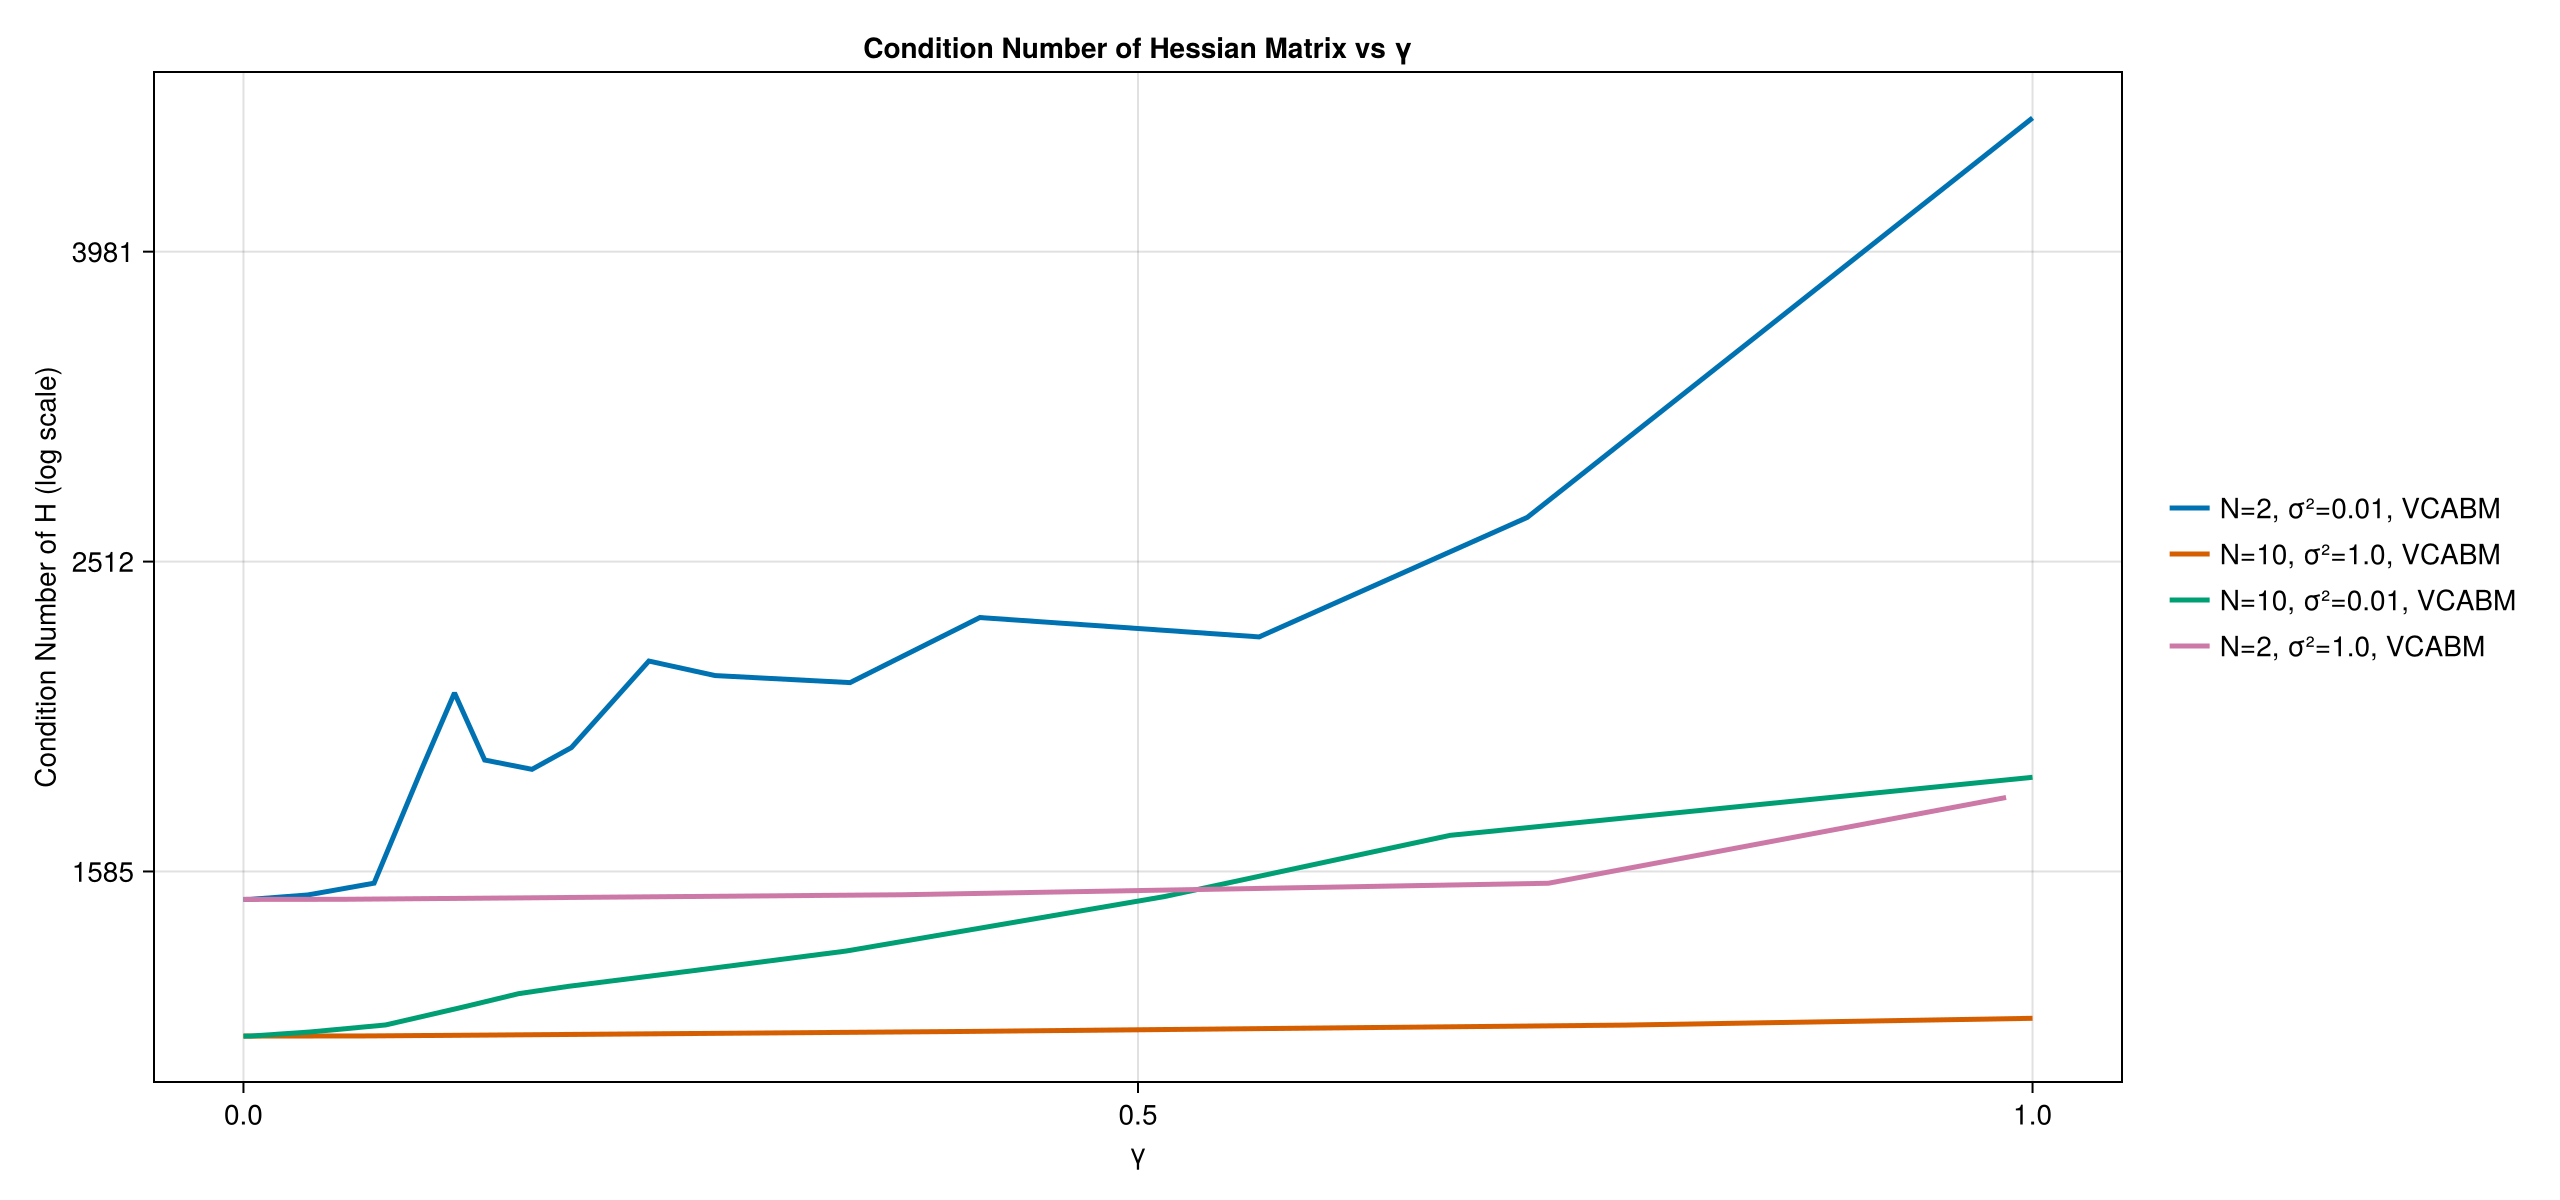
\includegraphics[width=0.9\textwidth]{./figures/condition_number_all.png}
	\caption{Condition number of matrix $\mH$.}
	\label{fig:condition_number}
\end{Figure}

% The results show that the condition number of $\mH$ generally remains below 3000. In addition, when the observation likelihood becomes narrower and the particles become more concentrated in space, the condition number increases accordingly.
To assess the numerical reliability of solving the linear system \(Ax=b\), it is useful to relate the condition number to the achievable accuracy. In finite-precision arithmetic, solving \(Ax=b\) typically loses about \(\log_{10}\kappa(A)\) decimal digits of accuracy. Therefore, a smaller condition number implies a more accurate numerical solution. Since the \texttt{Float64} type in Julia provides about 16 decimal digits of precision, the number of remaining significant digits can be approximated by
$\text{remaining significant digits} \approx 16 - \log_{10}\kappa(A)\enspace.$

\Fig{fig:condition_number} shows that the condition number of \(\mH\) generally remains below 3000. In addition, when the observation likelihood becomes narrower and the particles become more concentrated in space, the condition number increases accordingly. Since
$16 - \log_{10}(3000) \approx 12.5\enspace,$

the solution still retains about 12 significant digits even in the worst case considered here. Therefore, the numerical accuracy is more than sufficient for the MINRES solver tolerance of \(10^{-9}\), which confirms the practical feasibility of using MINRES in this study.

\begin{Figure}[ht]
	\centering
	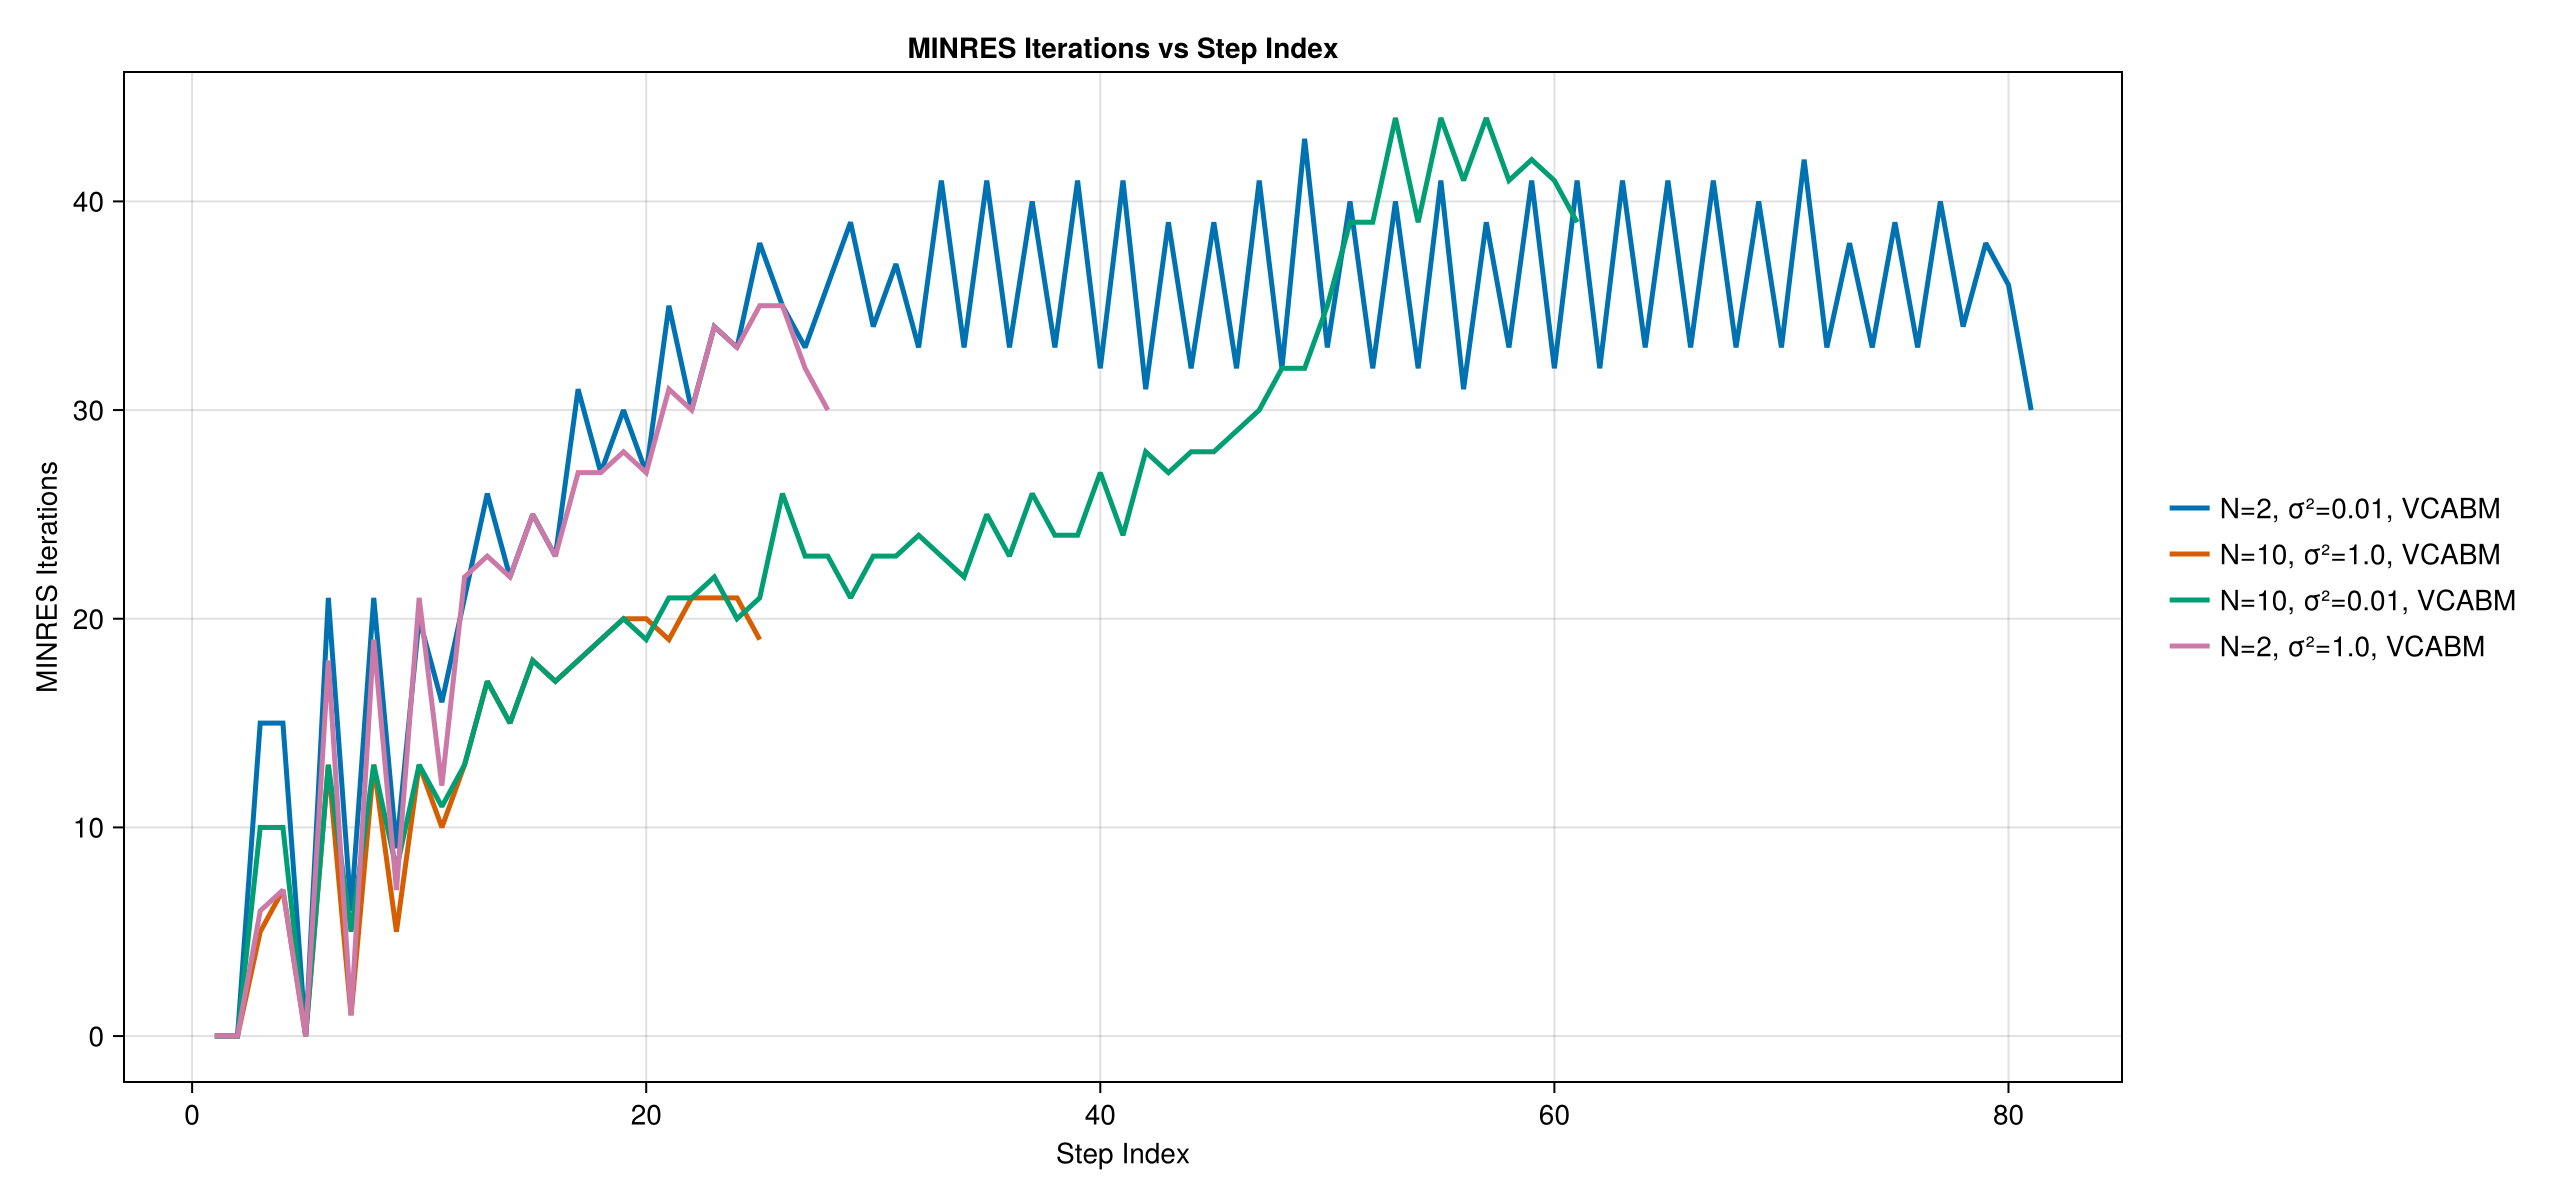
\includegraphics[width=0.9\textwidth]{./figures/minres_iterations_all.png}
	\caption{Number of iterations required for MINRES convergence.}
	\label{fig:minres_iterations}
\end{Figure}

Within the observed range of condition numbers, MINRES converges rapidly. In \Fig{fig:minres_iterations}, the iteration count $k$ usually does not exceed 50. Specifically, for a 2D system with 1000 particles (matrix dimension 2000), the relation $50 \ll \frac{2000}{3} \approx 667$ holds. For a 10D system with 1000 particles (matrix dimension 10000), the relation becomes $50 \ll \frac{10000}{3} \approx 3333$. These results demonstrate that MINRES is highly efficient for high-dimensional systems compared with Cholesky-based methods.

Furthermore, the iterative nature of MINRES naturally enables a warm-start strategy. When the integrator uses very small steps in $\gamma$, the changes in the system matrix $\mH$ and the vector $\mJ$ are also small. Therefore, this study uses the velocity $\dot{\eta}(\gamma^*)$ from the previous virtual-time step $\gamma^*$ as the initial guess for MINRES. Although the strict convergence tolerance ($10^{-9}$) limits the warm-start gain to only 1--2 iterations per call, the frequent use of MINRES during the integration of $\mH(\gamma)\dot{\eta}(\gamma) = -\mJ(\gamma)$ leads to a substantial cumulative reduction in the total number of matrix--vector products.

Since the Hessian matrix $\mH$ is symmetric and positive definite, the Conjugate Gradient (CG) method is also a viable option for solving the linear system. However, MINRES is preferred in this study because of its superior numerical stability while maintaining a computational speed comparable to that of CG.

\subsection{ODE Integrator Selection for Continuous Smooth Flow: The VCABM Method}
\label{subsec:vcabm}

When integrating the ODE $\mH(\gamma)\dot{\eta}(\gamma) = -\mJ(\gamma)$ from 0 to 1, the choice of numerical integrator depends mainly on the stiffness of the equation. If the system is highly stiff, even a small deviation of the particle position $\eta(\gamma)$ from the true trajectory can cause the evolution rate $\dot{\eta}(\gamma)$ to change sharply, making the numerical error grow rapidly \cite{NME}. To maintain stability, the integrator is then forced to use very small step sizes.

The stiffness of the ODE depends not only on the shape of the observation likelihood function $f_L(\vx)$, i.e., the variance of the measurement noise, but also on the geometric position of the particles relative to the likelihood. This dynamic relationship can be understood from the formula for the derivative of the true posterior weights with respect to virtual time
$$\dot{w}_i(\gamma)=\frac{\dot g(\gamma)\ln(f_L(\vx_i))}{L}-\frac{\sum_{j=1}^L \dot g(\gamma)\ln(f_L(\vx_j))}{L^2}\enspace.$$
Assuming a Gaussian observation likelihood, its log-likelihood $\ln(f_L(\vx))$ is geometrically a downward-opening parabola, or a high-dimensional paraboloid. The stiffness of the ODE depends on which region of this curve the particles occupy:

\textbf{Steep region far from the center (high stiffness):} If the prior particles are initially far from the effective likelihood region, they lie on the outer parts of the parabola. Since the outer regions of a quadratic function are steep, even a very small shift in the particle position $\vx_i$ causes a large change in $\ln(f_L(\vx_i))$. This sensitivity leads to a large variation in $\dot{w}_i(\gamma)$, which in turn induces significant changes in $\dot{\eta}$.

\textbf{Flat region near the center (low stiffness):} As virtual time progresses, the particles gradually flow toward the center of the likelihood, where the parabola becomes flatter. In this region, the log-likelihood is much less sensitive to small changes in particle position. Consequently, the value of $\dot{w}_i(\gamma)$ becomes more stable. Changes in the particle position $\eta$ no longer cause sharp jumps in $\dot{\eta}$, and the stiffness of the ODE decreases substantially.

This study uses the VCABM (Variable-Coefficient Adams--Bashforth--Moulton) multistep predictor--corrector integrator \cite{NME}. Its basic principle is as follows: at the beginning, the algorithm starts with small steps and collects sufficient historical information to construct a polynomial approximation. It then uses this polynomial to predict the particle position $\eta_{\mathrm{pre}}$ at the next virtual-time step and computes the flow rate $\dot{\eta}_{\mathrm{pre}}$ at the predicted point. Based on $\dot{\eta}_{\mathrm{pre}}$, the predictor is corrected to obtain the final value.

For highly stiff ODEs, even a slight deviation of the predicted position $\eta_{\mathrm{pre}}$ from the true trajectory can cause the computed flow rate $\dot{\eta}_{\mathrm{pre}}$ to become very large. This leads to a large discrepancy between the predicted and corrected values. If the discrepancy exceeds the tolerance, VCABM rejects the step and significantly reduces the step size $\Delta \gamma$ before retrying. In contrast, for weakly stiff ODEs, the predicted and corrected values remain close to each other, so the integrator can enlarge the step size and complete the integration more quickly.

To verify the suitability of VCABM, this study tests four cases in 2D and 10D systems($N=2,\enspace N=10$). In these experiments, the prior is a standard normal distribution, and the likelihood mean is $[3, 3, \dots]$. Likelihood variances of $\sigma^2 = 1.0$ (wide likelihood) and $\sigma^2 = 0.01$ (narrow likelihood) are used. Then use the VCABM integrator to calculate the integral value\Eq{eq:eta_flow_prior_posterior}. The experiments track the cumulative evolution of virtual time $\gamma$ as a function of the number of integration steps.

\begin{Figure}[ht]
	\centering
	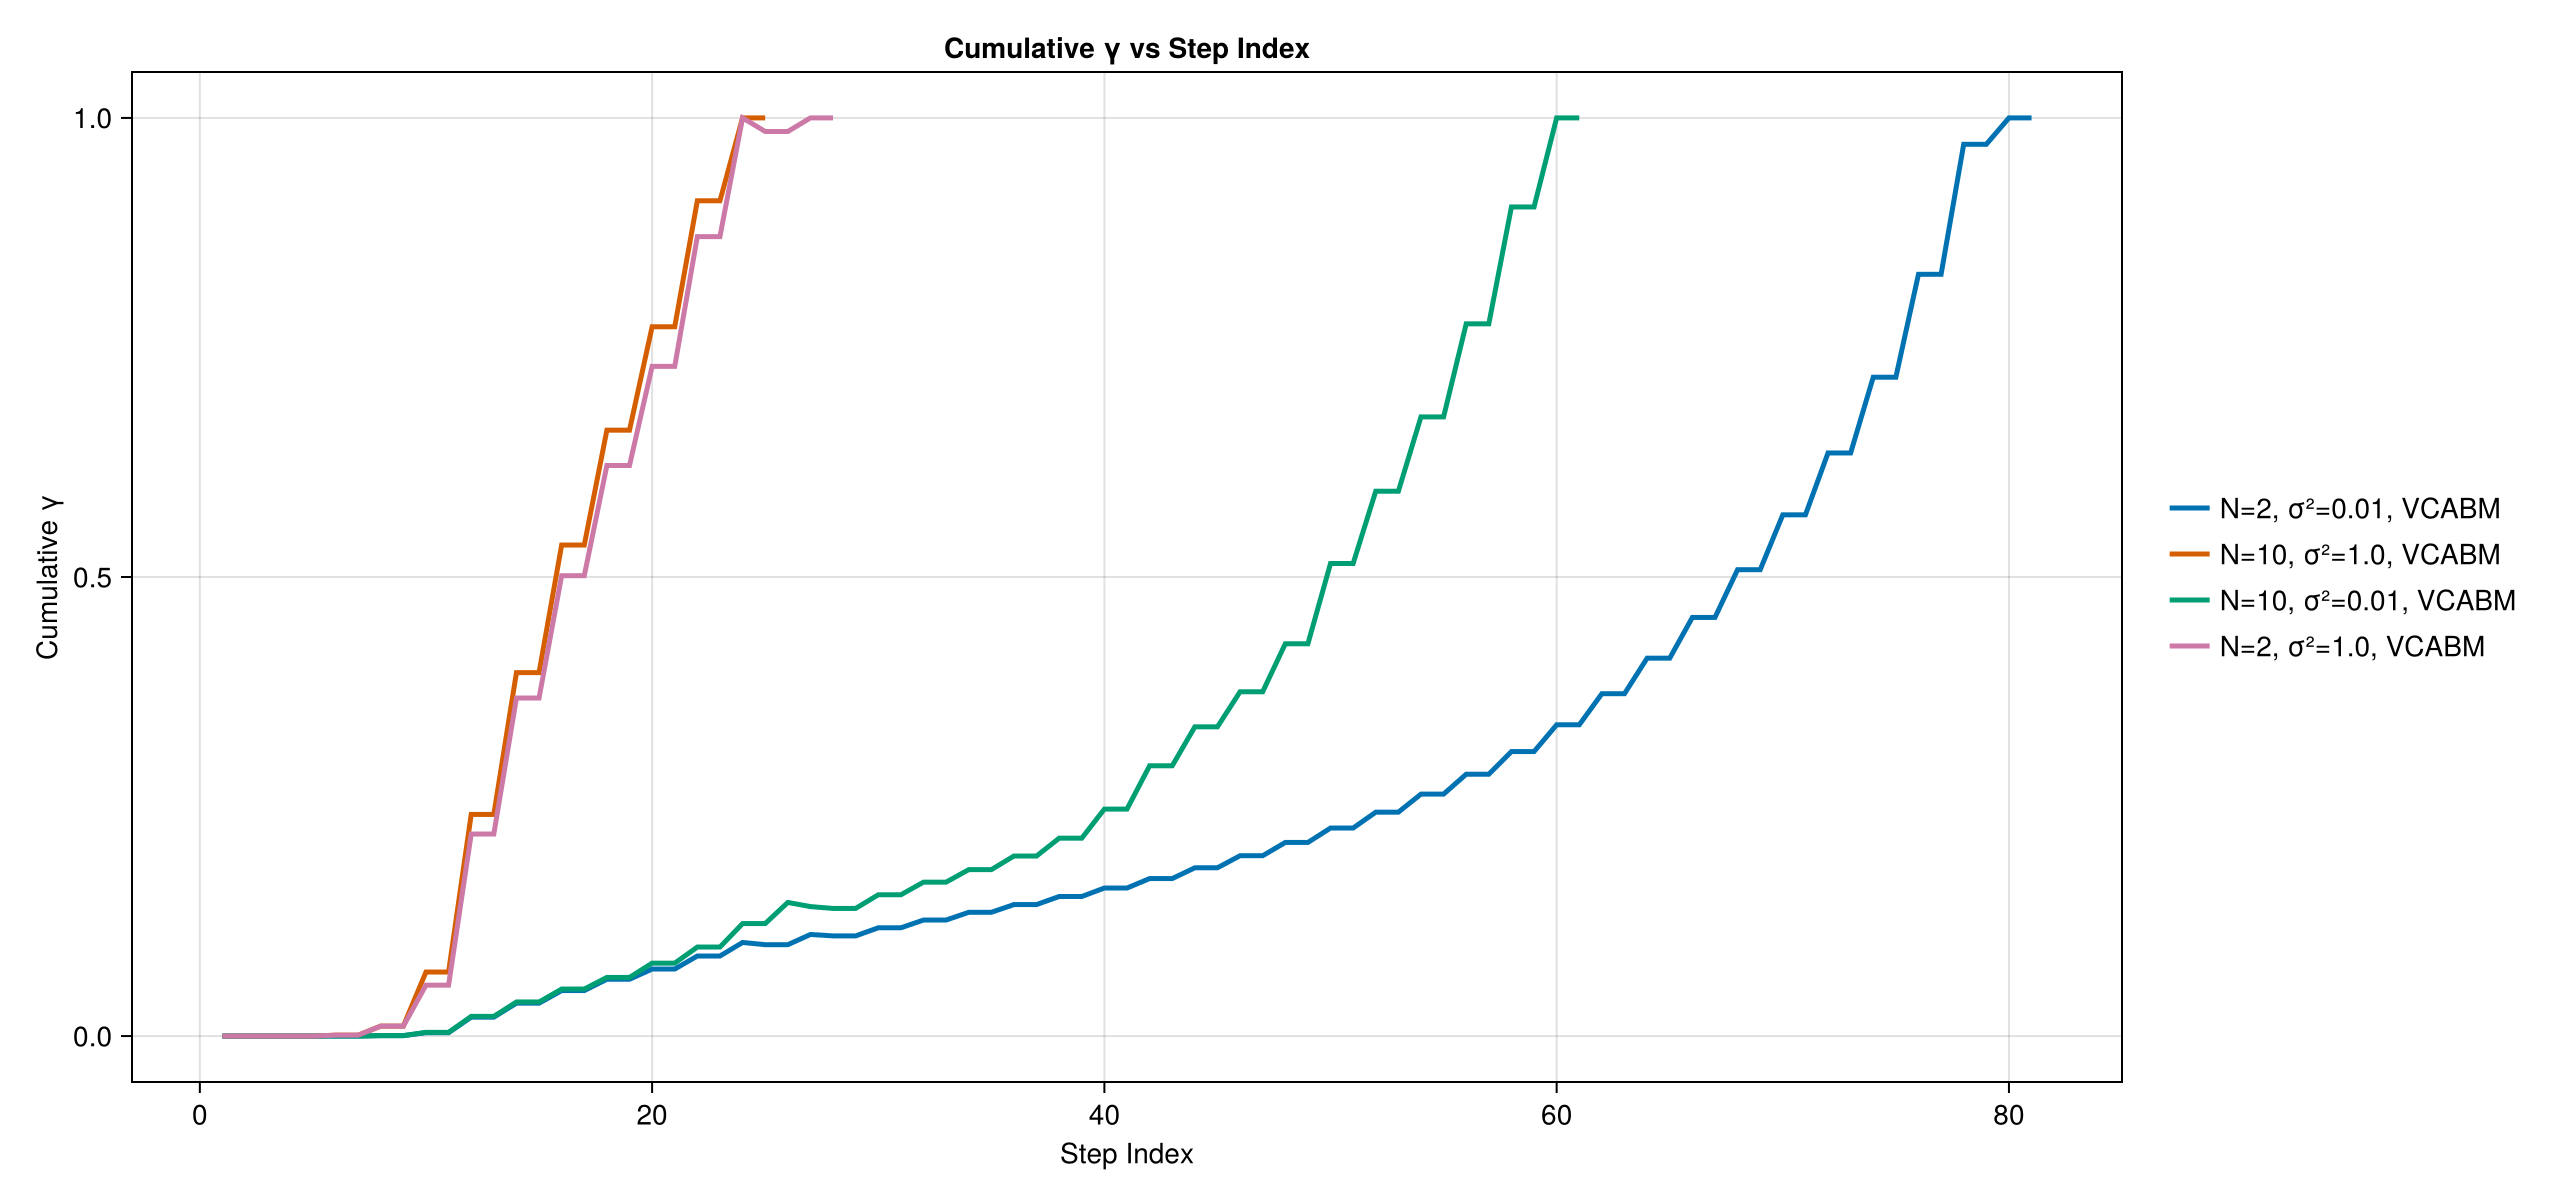
\includegraphics[width=0.85\textwidth]{./figures/cumulative_gamma_all.png}
	\caption{$\gamma$ vs. integration steps.}
	\label{fig:cumulative_gamma}
\end{Figure}

The experimental results in \Fig{fig:cumulative_gamma} agree with the theoretical analysis. When the likelihood variance is 1.0, the likelihood function is relatively flat, and the ODE stiffness remains low. VCABM can therefore use large step sizes consistently and completes the integration from $\gamma = 0$ to $1$ in fewer than 50 steps.

When the likelihood variance decreases to 0.01, the sharper likelihood function makes the ODE substantially stiffer. As a result, the integrator must use very small steps initially, increasing the total step count to around 100. Even though highly informative observations increase the numerical stiffness, the ODE remains within a regime that standard integrators can still handle effectively.

\section{Matrix-Free Method Based on MINRES}
\label{sec:matrix_free}

The implementation described above still requires storing the full Hessian matrix $\mH$ in GPU memory. However, storing the full Hessian introduces a severe memory bottleneck.

The dimension of $\mH$ is $NL \times NL$, so its memory requirement grows quadratically with both $N$ and $L$. For example, when $N=10$ and $L=2000$, the matrix $\mH$ has dimension $20000 \times 20000$. Using 64-bit floating-point numbers (\texttt{Float64}), this matrix alone occupies approximately 3.2~GB of GPU memory.

In practical engineering tests, parallel simulations are often required to evaluate the overall performance of the filter. If the system dimension and the particle number are increased further, or if multiple NFF instances run on the GPU simultaneously, this large matrix will quickly exhaust the available GPU memory. This leads to out-of-memory errors and makes large-scale parallel validation infeasible.

To overcome this bottleneck, the specific properties of MINRES can be exploited. As discussed in \Sec{subsec:minres}, during the iterative solution of $\mH\dot{\eta} = -\mJ$, MINRES does not need access to every individual element of $\mH$. Instead, it only requires the product of $\mH$ with an arbitrary vector $\vv$, i.e., the matrix--vector product $\mH\vv$.

Based on this fact, it is possible to avoid constructing and storing $\mH$ entirely. Instead, an analytical function can be derived that directly evaluates the product $\mH\vv$.

The matrix-free derivation of $\mH\vv$ is as follows.

For the $k$-th vector block $\vu_k$ (where $k \in \{1, 2, \dots, L\}$), the expression is
\begin{equation}
	\vu_k = (\mH\vv)_k = \sum_{j=1}^L \mH_{kj}\vv_j \enspace .
\end{equation}

Based on the blockwise form of the Hessian matrix in \Eq{eq:Hkl}, the off-diagonal and diagonal blocks can be treated in a unified way. Substituting $\mH_{kl} = 2w^2 \{ K\mI_N - 2\mathcal{H}(\vx_k - \vx_l) \}$ into the equation above yields
\begin{equation}
	\vu_k = 2w^2 \left( K \sum_{j=1}^L \vv_j - 2 \sum_{j=1}^L \mathcal{H}(\vx_k - \vx_j)\vv_j \right) \enspace .
\end{equation}

Substituting \Eq{eq:h} into the expression for $\vu_k$ and expanding it gives
\begin{equation}
	\vu_k = 2w^2 K \sum_{j=1}^L \vv_j - 8w^2 \sum_{j=1}^L \frac{2d_{\text{min}}^2 + \vd^{\top}\vd}{(d_{\text{min}}^2 + \vd^{\top}\vd)^2} \vd\vd^{\top} \vv_j - 4w^2 \sum_{j=1}^L \left[ \frac{\vd^{\top}\vd}{d_{\text{min}}^2 + \vd^{\top}\vd} + \log(d_{\text{min}}^2 + \vd^{\top}\vd) \right] \vv_j \enspace .
\end{equation}

By grouping similar terms, two scalar coefficients, $\alpha_{kj}$ and $\beta_{kj}$, can be defined as
\begin{align}
	\alpha_{kj} &= 2w^2 K - 4w^2 \frac{\vd^{\top}\vd}{d_{\text{min}}^2 + \vd^{\top}\vd} - 4w^2 \log(d_{\text{min}}^2 + \vd^{\top}\vd) \enspace , \\
	\beta_{kj} &= 8w^2 \frac{2d_{\text{min}}^2 + \vd^{\top}\vd}{(d_{\text{min}}^2 + \vd^{\top}\vd)^2} \enspace .
\end{align}

Using these two scalar coefficients, the expression for $\vu_k$ simplifies to
\begin{equation}
	\vu_k = \sum_{j=1}^L \alpha_{kj} \vv_j - \sum_{j=1}^L \beta_{kj} (\vd_{kj}^{\top} \vv_j) \vd_{kj} \enspace .
\end{equation}

If the second-moment penalty mechanism introduced earlier is included, the Hessian matrix becomes $\mH^{\mathrm{new}} = \mH^{\mathrm{original}} + \mH^{\mathrm{cov}}$, where the additional covariance block is
\begin{equation}
	\mH_{kl}^{\mathrm{cov}} = 4K_{\mathrm{cov}}w^2 \left( (\vx_k^{\top} \vx_l)\mI_N + \vx_l \vx_k^{\top} \right) \enspace .
\end{equation}
Accordingly,
\begin{equation}
	(\mH^{\mathrm{new}}\vv)_k = \vu_k^{\mathrm{original}} + \sum_{j=1}^L 4K_{\mathrm{cov}}w^2 \left( (\vx_k^{\top} \vx_j)\vv_j + (\vx_k^{\top} \vv_j)\vx_j \right) \enspace .
\end{equation}

MINRES typically requires tens of iterations, meaning that the matrix-free product $\mH\vv$ must be evaluated many times. However, the scalars $\alpha_{kj}$ and $\beta_{kj}$ depend only on the particle positions $\vx$ at the current virtual time and therefore remain constant during a single MINRES solve.

Therefore, when computing the vector $\mJ$, the coefficients $\alpha_{kj}$ and $\beta_{kj}$ can be precomputed and stored in two $L \times L$ scalar matrices $\mA$ and $\mB$, where $\mA_{kj} = \alpha_{kj}$ and $\mB_{kj} = \beta_{kj}$. In the subsequent MINRES iterations, the algorithm no longer needs to recompute the expensive kernel expressions. Instead, it only performs matrix lookups, dot products, and vector operations. This matrix-free scheme reduces the memory complexity from $O((NL)^2)$ to $O(L^2)$.

\section{NFF Prediction Step}
\label{sec:prediction_step}

The previous sections described the update step of NFF. However, a complete nonlinear filtering procedure also requires a prediction step. This study implements the following three prediction methods.

\subsection{Method 1}
\label{subsec:method1}

The first prediction mechanism is identical to the prediction step used in PF. For the $L$ posterior particles obtained after the update step at time $k-1$, the algorithm draws a random noise sample $\vv_{k-1}^{(i)}$ from the process noise distribution $\mathcal{N}(\mathbf{0}, \mQ)$ for each particle $\vx_{k-1}^{(i)}$.

Each particle is then propagated by one step through the discretized system evolution equation together with its corresponding noise sample, yielding $L$ new prior particles given by
\begin{equation}
	\vx_k^{(i)} = f_k(\vx_{k-1}^{(i)}, \vv_{k-1}^{(i)}), \quad i = 1, 2, \dots, L \enspace .
\end{equation}

\subsection{Method 2}
\label{subsec:method2}

The second prediction method begins by deterministically extracting $K$ fixed noise samples $\vv_{k-1}^{(j)}$ ($j = 1, 2, \dots, K$) from the process noise distribution $\mathcal{N}(\mathbf{0}, \mQ)$. Next, each posterior particle from the previous time step is combined with all $K$ noise samples and propagated forward. This is equivalent to taking the Cartesian product of the state particles and the noise samples, resulting in a total of $L \times K$ predicted points using
\begin{equation}
	\vx_k^{(i,j)} = f_k(\vx_{k-1}^{(i)}, \vv_{k-1}^{(j)}), \quad i = 1, \dots, L, \quad j = 1, \dots, K \enspace ,
\end{equation}
where $\vx_{k-1}^{(i)}$ denotes the $i$-th posterior particle at time $k-1$. After generating this set of $L \times K$ points, the algorithm applies an optimal reduction procedure. This procedure treats the $L \times K$ points as a fixed reference distribution and optimizes $L$ equally weighted particles by minimizing the modified \ac{cvm} between the optimized set and the reference set. The resulting $L$ particles serve as the prior distribution at the current time step.

\begin{Figure}[ht]
	\centering
	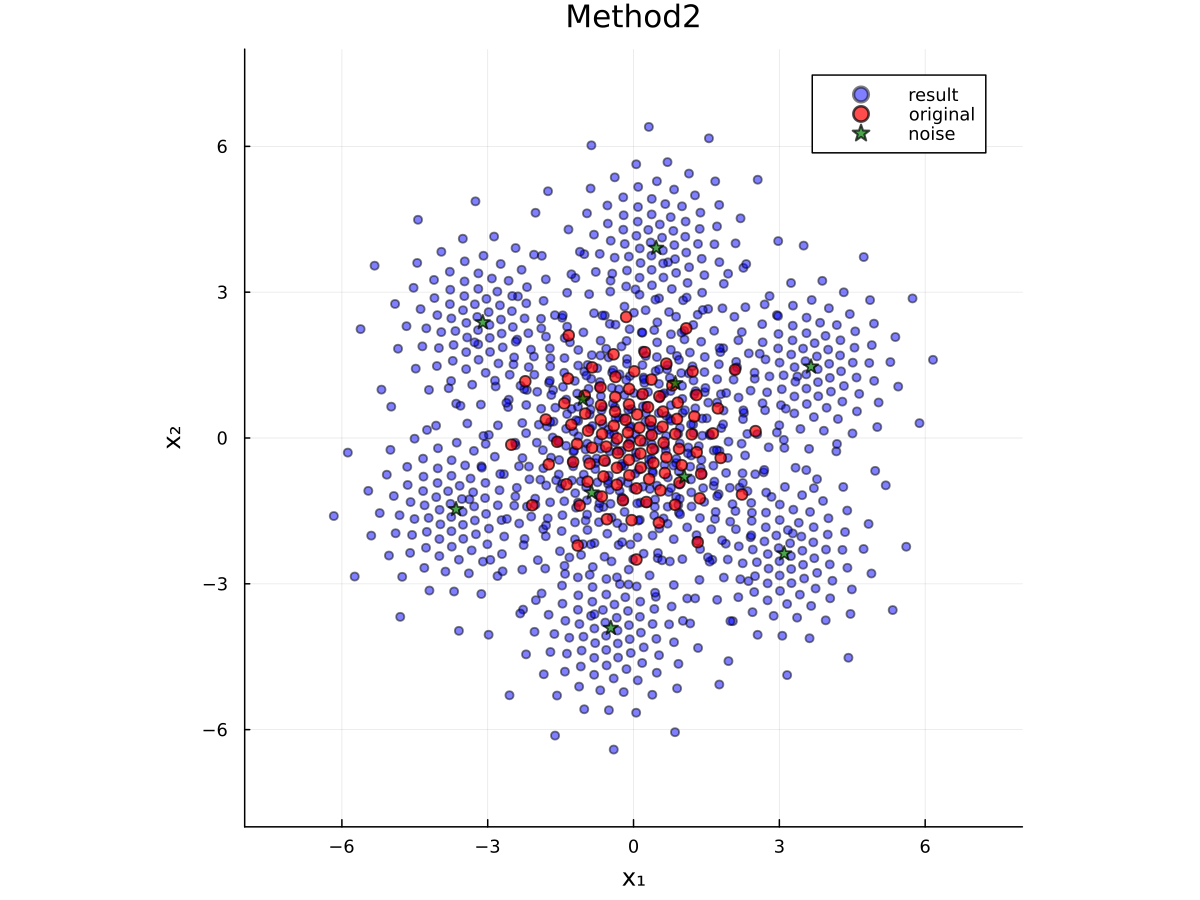
\includegraphics[width=0.9\textwidth]{figures/Examples/method2_final.png}
	\caption{Visualization of Method 2.}
	\label{fig:method2_viz}
\end{Figure}
\clearpage

\subsection{Method 3}
\label{subsec:method3}

In this method, the algorithm concatenates the $L$ particles of dimension $N$ from the current posterior into a single high-dimensional particle of dimension $L \times N$. At the same time, the process noise distribution is lifted to an $L \times N$-dimensional Gaussian distribution
\[
\mathcal{N}(\mathbf{0}, \text{diag}(\mQ, \dots, \mQ)) \enspace ,
\]
whose covariance is block diagonal with $L$ copies of $\mQ$.

In this high-dimensional noise space, the algorithm deterministically extracts $K$ high-dimensional noise samples $\vv_{k-1}^{(j)}$ ($j = 1, 2, \dots, K$). The current high-dimensional particle is then propagated through the system equations using each of these $K$ noise samples, yielding $K$ high-dimensional particles given by
\begin{equation}
	\begin{bmatrix} \vx_k^{(1, j)} \\ \vdots \\ \vx_k^{(L, j)} \end{bmatrix} = \begin{bmatrix} f_k(\vx_{k-1}^{(1)}, \vv_{k-1}^{(j, 1)}) \\ \vdots \\ f_k(\vx_{k-1}^{(L)}, \vv_{k-1}^{(j, L)}) \end{bmatrix}, \quad j = 1, 2, \dots, K \enspace ,
\end{equation}
where $\vv_{k-1}^{(j, i)}$ denotes the components of the $j$-th high-dimensional noise sample from dimension $(i-1)N + 1$ to $iN$.

After obtaining these $K$ high-dimensional particles, each one is split into $L$ separate $N$-dimensional particles. In this way, the $K$ super-particles are effectively transformed into $K \times L$ particles of dimension $N$. Finally, the optimal reduction algorithm reduces these $K \times L$ particles back to $L$ particles, thereby completing the prediction step.

\begin{Figure}[ht]
	\centering
	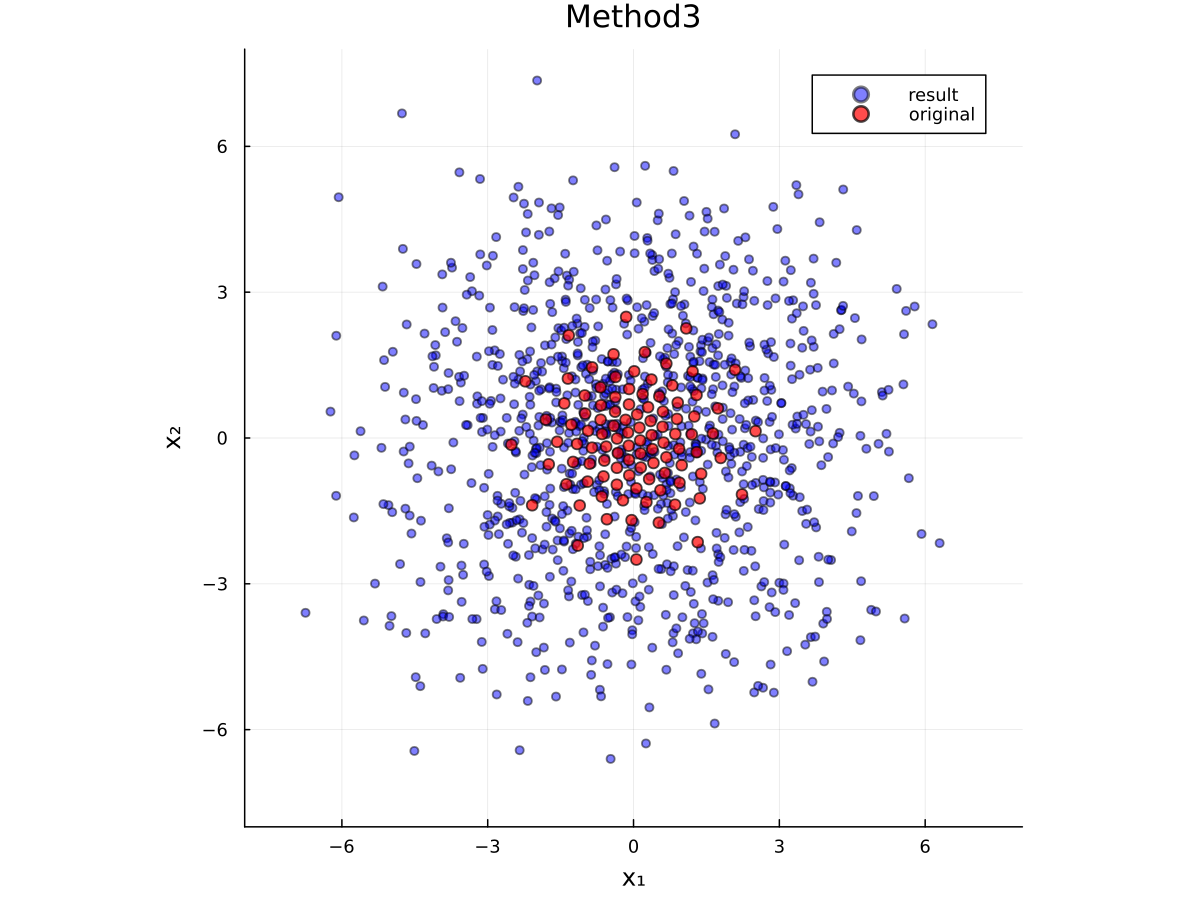
\includegraphics[width=0.8\textwidth]{figures/Examples/method1_final.png}
	\caption{Visualization of Method 3.}
	\label{fig:method3_viz}
\end{Figure}

\clearpage

\subsection{Prediction Step for the Lorenz 96 System}
\label{subsec:lorenz96_prediction}

When discretizing the Lorenz 96 system, the total perturbation over the macroscopic integration step $\Delta t$ must first be determined. For the stochastic noise term in the system equation, this requires integrating the standard Wiener process increment $d\mW_t$ over the interval $[t_{k-1}, t_k]$ as
\begin{equation}
	\vv_{k-1} = \int_{t_{k-1}}^{t_k} \mG d\mW_t \enspace .
\end{equation}
The multidimensional standard Wiener process can be interpreted as follows: at every infinitesimal time interval $dt$, the system is perturbed by an independent Gaussian increment $\Gaussian(\vzero, \mI dt)$ with an infinitesimal covariance. Integrating the Wiener process over an interval of length $\Delta t$ amounts to a continuous superposition of infinitely many independent Gaussian increments. By the additivity of independent Gaussian random variables, the sum remains Gaussian, and the total covariance equals the sum of the infinitesimal covariances, i.e., $\sum \mI dt = \mI \Delta t$. Therefore, over the macroscopic step $\Delta t$, the cumulative process noise $\vv_{k-1}$ follows
\begin{equation}
	\vv_{k-1} \sim \Gaussian\left(\vzero, \Delta t \mG \mG^{\top}\right) \enspace .
\end{equation}

In Method 1 described in \Sec{subsec:method1}, the algorithm uses purely stochastic sampling. To simulate the Lorenz 96 system accurately, Method 1 adopts the standard Euler--Maruyama (EM) scheme. EM divides the macroscopic step $\Delta t$ into $M$ microscopic substeps of size $dt = \Delta t / M$. At each microscopic time step $m$, the algorithm generates a new independent Gaussian increment $\Delta \mW_m \sim \Gaussian(\vzero, \mI dt)$ and updates the state according to
\begin{equation}
	\vx_{m+1} = \vx_m + \vf(\vx_m)dt + \mG\Delta \mW_m \quad (m = 0, 1, \dots, M-1) \enspace .
\end{equation}
Since the increments $\Delta \mW_m$ are mutually independent, after $M$ steps the accumulated variance becomes $M \times dt \mG\mG^{\top} = \Delta t \mG\mG^{\top}$.

When deterministic sampling is introduced in Method 2 and Method 3, the algorithm must deterministically extract $K$ sample points $\vv^{(k)}$ ($k = 1, 2, \dots, K$) from the macroscopic process noise distribution $\Gaussian(\vzero, \Delta t \mG\mG^{\top})$. At this point, a common engineering pitfall arises. If one propagates the particles over $\Delta t$ using only the drift term $\vf(\vx_t)$ and then simply adds the extracted macroscopic noise samples $\vv^{(k)}$ afterward, this procedure completely ignores the continuous influence of the stochastic term on the nonlinear trajectory during the interval $\Delta t$.

To address this issue, this study replaces the stochastic EM paths with deterministic straight-line paths. In the standard Euler--Maruyama method, the noise path starts at $\vzero$ and ends at a random sample drawn from $\Gaussian(\vzero, \Delta t \mG\mG^{\top})$. Here, by contrast, each deterministically extracted macroscopic noise sample $\vv^{(k)}$ is interpreted as a straight-line path from $\vzero$ to $\vv^{(k)}$ in the noise space. Across the $M$ microscopic substeps, the algorithm injects the incremental component of this path, i.e., $\frac{\vv^{(k)}}{M}$, at each step. The update formula becomes
\begin{equation}
	\tilde{\vx}_{m+1} = \tilde{\vx}_m + \vf(\tilde{\vx}_m) dt + \frac{\vv^{(k)}}{M} \qquad (m = 0, 1, \dots, M-1) \enspace .
\end{equation}
After $M$ microscopic steps, the final propagated state is $\vx_{t+\Delta t} = \tilde{\vx}_M$. In this way, each prior particle evolves along $K$ different deterministic straight-line paths. Because the noise is injected throughout the nonlinear integration process, the dynamic coupling between the stochastic term and the system evolution is effectively preserved.

\begin{Figure}[ht]
	\centering
	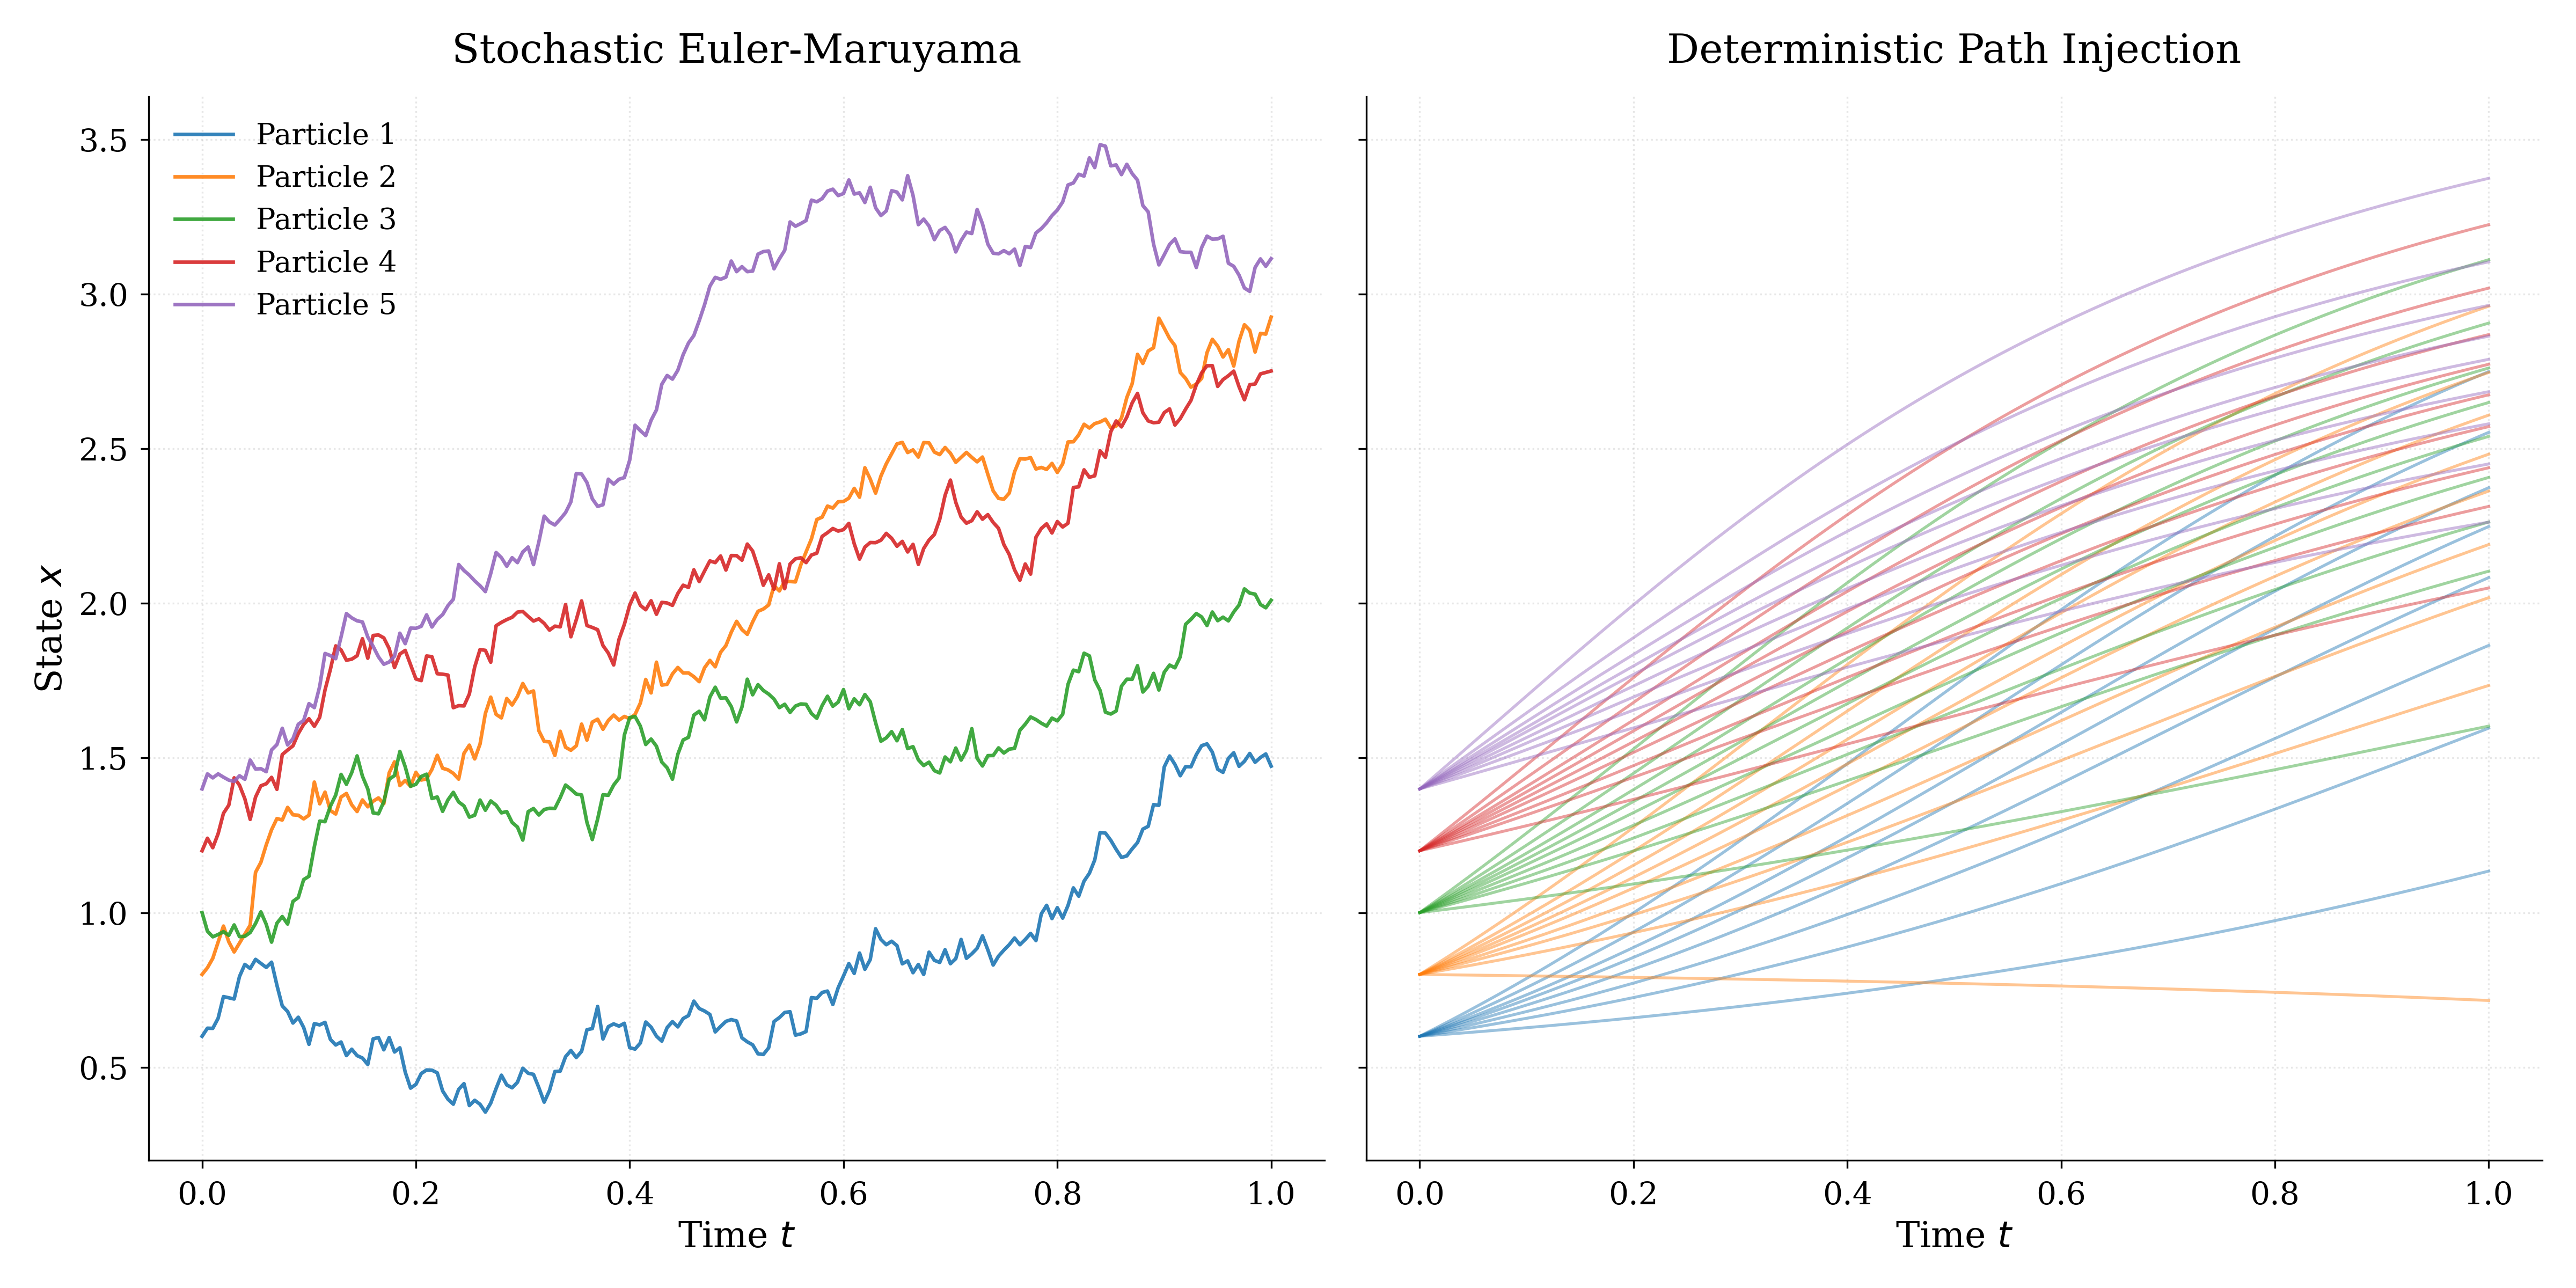
\includegraphics[width=0.95\textwidth]{figures/nonlinear_comparison.png}
	\caption{Comparison of noise injection strategies in the prediction step. }
	\label{fig:sde_comparison}
\end{Figure}

As shown in the \Fig{fig:sde_comparison}, the deterministic noise injection method enables a more uniform exploration of the state space, thereby capturing significantly more predictive information.

Within this straight-line path framework, the main difference between Method 2 and Method 3 lies in the independence of the paths. In Method 2, deterministic sampling is performed in a low-dimensional space, so all $L$ particles share the same $K$ straight-line evolution paths. In Method 3, deterministic sampling is performed in an extremely high-dimensional space, so each particle has its own set of $K$ exclusive straight-line evolution paths, completely independent of those of the other particles.

\subsection{Numerical Overflow and Acceleration Strategies for High-Dimensional Deterministic Sampling}
\label{subsec:overflow_strategies}

In Method 3 described in \Sec{subsec:method3}, deterministic sampling must be performed in a space of dimension $N \times L$, which is typically greater than 10,000. This is done by minimizing the modified Cramér--von Mises distance between a Gaussian distribution and a Dirac mixture distribution \cite{LCDSM}. However, when evaluating the distance $D$ and its gradient $G$ in such high dimensions, serious numerical overflow and efficiency bottlenecks arise.

According to Dirac mixture approximation theory for multivariate Gaussian distributions, the modified CVM distance $D$ between a Gaussian distribution $\tilde{f}$ and a Dirac mixture $f$ can be decomposed into three parts as
\begin{equation}
	D = D_1 - 2D_2 + D_3, \quad \text{where} \quad D_i = \int_0^{b_{\max}} \frac{1}{b^{N-1}} P_i \dd b \quad (i = 1, 2, 3) \enspace .
\end{equation}
Here, $D_1$ is a constant independent of the Dirac mixture and can therefore be ignored during optimization. The expressions for $P_2$ and $D_3$ are
\begin{equation}
	P_2 = (2\pi)^{\frac{N}{2}} b^{2N} \left( \prod_{k=1}^N \frac{1}{\sqrt{(\sigma^{(k)})^2 + 2b^2}} \right) \sum_{i=1}^L w_i \exp\!\left( -\frac{1}{2} \sum_{k=1}^N \frac{(x_i^{(k)})^2}{(\sigma^{(k)})^2 + 2b^2} \right) \enspace ,
\end{equation}
\begin{equation}
	D_3 = \frac{\pi^{\frac{N}{2}}}{8} \sum_{i=1}^L \sum_{j=1}^L w_i w_j \Big( 4b_{\max}^2 - C_b T_{ij} + T_{ij}\log(T_{ij}) \Big) \enspace ,
\end{equation}
where $T_{ij} = \sum_{k=1}^N (x_i^{(k)} - x_j^{(k)})^2$ and the constant $C_b = \log(4b_{\max}^2) - \Gamma$. To determine the optimal particle locations $\vx$ that minimize the distance, the partial derivative of the distance function with respect to the $\eta$-th component of the $\xi$-th particle, $x_\xi^{(\eta)}$, is derived as $G_\xi^{(\eta)} = G_\xi^{(\eta, 1)} + G_\xi^{(\eta, 2)}$, where
\begin{equation}
\begin{split}
    G_\xi^{(\eta, 1)} = {} & 2(2\pi)^{\frac{N}{2}} w_\xi x_\xi^{(\eta)} \int_0^{b_{\text{max}}} \frac{b^{N+1}}{(\sigma^{(\eta)})^2 + 2b^2} \left( \prod_{k=1}^N \frac{1}{\sqrt{(\sigma^{(k)})^2 + 2b^2}} \right) \text{\raisebox{-.7\baselineskip}[0pt][0pt]{\rotatebox[origin=c]{180}{$\Rsh$}}} \\
    & \exp\!\left( -\frac{1}{2} \sum_{k=1}^N \frac{(x_\xi^{(k)})^2}{(\sigma^{(k)})^2 + 2b^2} \right) \dd b \enspace ,
\end{split}
\end{equation}
\begin{equation}
	G_\xi^{(\eta, 2)} = \frac{\pi^{\frac{N}{2}}}{2} w_\xi \left\{ \sum_{i=1}^L w_i (x_\xi^{(\eta)} - x_i^{(\eta)}) \log\left( \sum_{k=1}^N (x_\xi^{(k)} - x_i^{(k)})^2 \right) + C_b \left( \sum_{i=1}^L w_i x_i^{(\eta)} - x_\xi^{(\eta)} \right) \right\} \enspace .
\end{equation}

As shown above, the terms $D_2$, $D_3$, and the gradients $G^{(1)}$, $G^{(2)}$ all contain the constant factor $\pi^{N/2}$. Since this factor does not affect the optimizer, it can be omitted during optimization.

When the dimension $N$ reaches 10,000, terms such as $b^{N+1}$ in the integral cause severe numerical overflow. To handle this problem, this study applies a logarithmic transformation. Using this log trick, the powers and products in the kernel of the $D_2$ integral are rewritten in the form $\exp(\ln(\cdot))$ as
\begin{equation}
	\begin{split}
		D_2 = \int_0^{b_{\text{max}}} &\exp\!\left( (N+1)\ln b + \frac{N}{2}\ln 2 - \sum_{k=1}^N \frac{1}{2} \ln((\sigma^{(k)})^2 + 2b^2) \right) \text{\raisebox{-.7\baselineskip}[0pt][0pt]{\rotatebox[origin=c]{180}{$\Rsh$}}} \\
		&\cdot \sum_{i=1}^L w_i \exp\!\left( -\frac{1}{2} \sum_{k=1}^N \frac{(x_i^{(k)})^2}{(\sigma^{(k)})^2 + 2b^2} \right) \dd b \enspace .
	\end{split}
\end{equation}

Similarly, for the gradient term $G_\xi^{(\eta, 1)}$, after factoring out the external constants, the integral kernel can be rewritten in a numerically safe form as
\begin{equation}
	\begin{split}
		G_\xi^{(\eta, 1)} \propto \int_0^{b_{\text{max}}} & \exp\! \bigg( (N+1)\ln b + \left(\frac{N}{2}+1\right)\ln 2 - \ln((\sigma^{(\eta)})^2 + 2b^2) \text{\raisebox{-.7\baselineskip}[0pt][0pt]{\rotatebox[origin=c]{180}{$\Rsh$}}} \\
		& - \sum_{k=1}^N \frac{1}{2} \ln((\sigma^{(k)})^2 + 2b^2) \bigg) \cdot \exp\!\left( -\frac{1}{2} \sum_{k=1}^N \frac{(x_\xi^{(k)})^2}{(\sigma^{(k)})^2 + 2b^2} \right) \dd b \enspace .
	\end{split}
\end{equation}

In the implementation, the logarithmic terms are summed first. Because the large positive contribution from $(N+1)\ln b$ is offset by the large negative contribution from $-\sum \frac{1}{2}\ln(\cdot)$, the final exponent remains within a numerically stable range and avoids overflow.

Sampling $K$ points in a space of dimension $N \times L$ requires $N \times L \times K$ integration operations in each optimization step. For a problem of this scale, adaptive numerical integration would be prohibitively slow.

Therefore, this study uses a fixed-point integration scheme in the implementation. This method approximates the continuous integral by a finite weighted sum via
\begin{equation}
	\int f(b) \dd b \approx \sum_{i=1}^M c_i f(b_i) \enspace .
\end{equation}

To verify the performance of the three prediction mechanisms under different dimensions and noise conditions, as well as the feasibility of the improved LCD sampling code, a set of basic state-propagation experiments is designed. The discrete state transition equation used in the experiments is
\begin{equation}
	\vx_k = \vx_{k-1} + \vv_{k-1} \enspace ,
\end{equation}
where the posterior particles $\vx_{k-1}$ from the previous step are obtained by deterministic sampling from a standard normal distribution $\mathcal{N}(\mathbf{0}, \mI)$.

The experiments are conducted in low-dimensional settings (2D, $L=100$ particles) and high-dimensional settings (10D, $L=1000$ particles). Different process noise variances $\sigma^2 \in \{1.0, 2.0, 5.0, 10.0\}$ are also tested. The mean and covariance of the prior particles generated by the three prediction methods are compared with the true analytical solution, i.e., $\mathcal{N}(\mathbf{0}, \mI + \sigma^2\mI)$. The results are shown in \Tab{tab:cov_error} and \Tab{tab:mean_error}.

\begin{Table}[ht]
	\centering
	\small
	\begin{tabular}{|c|c|c|c|c|c|c|}
		\hline
		System Dim. & $\sigma^2$ & \multicolumn{3}{c|}{Method 1 (Stochastic)} & Method 2 & Method 3 \\ \cline{3-5}
		& & $L_{\mathrm{noise}}=10$ & $L_{\mathrm{noise}}=20$ & $L_{\mathrm{noise}}=50$ & ($L_{\mathrm{noise}}=10$) & ($L_{\mathrm{noise}}=10$) \\ \hline
		\textbf{2D}  & 1.0  & 0.0569 & 0.1013 & 0.0296 & \textbf{0.0035} & 0.0681 \\ \cline{2-7}
		($L=100$)    & 2.0  & 0.0658 & 0.1617 & 0.0606 & \textbf{0.0070} & 0.1362 \\ \cline{2-7}
		& 5.0  & 0.0843 & 0.3254 & 0.1576 & \textbf{0.0174} & 0.3406 \\ \cline{2-7}
		& 10.0 & 0.1673 & 0.5860 & 0.3236 & \textbf{0.0347} & 0.6812 \\ \hline
		\textbf{10D} & 1.0  & 0.1746 & \textbf{0.0996} & --     & 2.2350 & 0.1098 \\ \cline{2-7}
		($L=1000$)   & 2.0  & 0.2868 & \textbf{0.1648} & --     & 4.4700 & 0.2193 \\ \cline{2-7}
		& 5.0  & 0.6056 & \textbf{0.3644} & --     & 11.1750 & 0.5478 \\ \cline{2-7}
		& 10.0 & 1.1287 & \textbf{0.7094} & --     & 22.3500 & 1.0953 \\ \hline
	\end{tabular}
	\caption{Comparison of RFE\Eq{eq:Rfe} for different prediction mechanisms.}
	\label{tab:cov_error}
\end{Table}

\begin{Table}[ht]
	\centering
	\small
	\begin{tabular}{|c|c|c|c|c|c|c|}
		\hline
		System & Proc. Noise & \multicolumn{3}{c|}{Method 1 (Stochastic)} & Method 2 & Method 3 \\ \cline{3-5}
		Dim. & Var. ($\sigma^2$) & $L_{\mathrm{noise}}=10$ & $L_{\mathrm{noise}}=20$ & $L_{\mathrm{noise}}=50$ & ($L_{\mathrm{noise}}=10$) & ($L_{\mathrm{noise}}=10$) \\ \hline
		\textbf{2D}  & 1.0  & $1.63 \times 10^{-2}$ & $2.29 \times 10^{-2}$ & $1.93 \times 10^{-2}$ & $\bm{3.43 \times 10^{-6}}$ & $\bm{3.43 \times 10^{-6}}$ \\ \cline{2-7}
		($L=100$)    & 2.0  & $2.31 \times 10^{-2}$ & $3.24 \times 10^{-2}$ & $2.74 \times 10^{-2}$ & $\bm{3.43 \times 10^{-6}}$ & $\bm{3.43 \times 10^{-6}}$ \\ \cline{2-7}
		& 5.0  & $3.65 \times 10^{-2}$ & $5.12 \times 10^{-2}$ & $4.33 \times 10^{-2}$ & $\bm{3.43 \times 10^{-6}}$ & $\bm{3.43 \times 10^{-6}}$ \\ \cline{2-7}
		& 10.0 & $5.16 \times 10^{-2}$ & $7.24 \times 10^{-2}$ & $6.12 \times 10^{-2}$ & $\bm{3.42 \times 10^{-6}}$ & $3.43 \times 10^{-6}$ \\ \hline
		\textbf{10D} & 1.0  & $3.68 \times 10^{-2}$ & $2.48 \times 10^{-2}$ & --     & $7.54 \times 10^{-6}$ & $\bm{7.53 \times 10^{-6}}$ \\ \cline{2-7}
		($L=1000$)   & 2.0  & $5.20 \times 10^{-2}$ & $3.51 \times 10^{-2}$ & --     & $7.54 \times 10^{-6}$ & $\bm{7.53 \times 10^{-6}}$ \\ \cline{2-7}
		& 5.0  & $8.22 \times 10^{-2}$ & $5.54 \times 10^{-2}$ & --     & $7.54 \times 10^{-6}$ & $\bm{7.53 \times 10^{-6}}$ \\ \cline{2-7}
		& 10.0 & $1.16 \times 10^{-1}$ & $7.84 \times 10^{-2}$ & --     & $7.55 \times 10^{-6}$ & $\bm{7.53 \times 10^{-6}}$ \\ \hline
	\end{tabular}
	\caption{Comparison of mean error for different prediction mechanisms.}
	\label{tab:mean_error}
\end{Table}

Based on the experimental results, the following main conclusions can be drawn.

As shown clearly in \Tab{tab:mean_error}, Method 2 and Method 3, both of which use deterministic sampling, achieved mean errors close to zero. This indicates that they preserve the unbiasedness of the system evolution almost perfectly. In contrast, Method 1 exhibits a mean drift ranging from $10^{-2}$ to $10^{-1}$.

In the 2D system, Method 2 yields a very small covariance error. However, when the system dimension increases to 10D, the covariance error of Method 2 grows dramatically. Method 3, by contrast, remains highly robust, and its covariance estimation accuracy is substantially better than that of Method 2.

The reason for this difference is that Method 2 copies and shifts the same $K$ low-dimensional noise samples to all particle positions (see \Fig{fig:method2_viz}). This rigid construction becomes problematic in high-dimensional spaces. In contrast, Method 3 (see \Fig{fig:method3_viz}) performs independent noise sampling for each original particle. Therefore, only Method 1 and Method 3 are considered in the subsequent Lorenz 96 experiments.
	\chapter{Comparison of Update Performance Based on Gaussian Fusion Experiments}
\label{ch:gaussian_fusion}

To objectively evaluate the discrepancy between the outputs of the filters in the update step and the corresponding analytical solutions, this chapter designs a series of single-step Gaussian fusion experiments.

According to Bayes' theorem, when both the prior distribution and the likelihood are Gaussian, their fusion yields a posterior distribution with a closed-form analytical solution, which is also Gaussian. Suppose that the prior distribution of the state vector $\vx$ is $p(\vx) = \Gaussian(\vx \mid \vmu_p, \boldsymbol{\Sigma}_p)$, and that the likelihood can be written as a Gaussian with respect to $\vx$, i.e., $p(\vy|\vx) \propto \Gaussian(\vx \mid \vmu_L, \boldsymbol{\Sigma}_L)$. After multiplication and normalization, the resulting posterior is $p(\vx|\vy) = \Gaussian(\vx \mid \vmu_e, \boldsymbol{\Sigma}_e)$. Its posterior covariance and posterior mean satisfy \cite[Section~8.1.8]{MC}
\begin{equation}
	\boldsymbol{\Sigma}_e^{-1} = \boldsymbol{\Sigma}_p^{-1} + \boldsymbol{\Sigma}_L^{-1} \enspace ,
\end{equation}
and
\begin{equation}
	\vmu_e = \boldsymbol{\Sigma}_e \left( \boldsymbol{\Sigma}_p^{-1} \vmu_p + \boldsymbol{\Sigma}_L^{-1} \vmu_L \right) \enspace .
\end{equation}

All experiments in this chapter are conducted in a 10-dimensional state space. The prior distribution is fixed as a 10D standard normal distribution. Different likelihood distributions are then introduced by varying their parameters, such as the mean and variance, to represent sensor scenarios with different noise levels and mean shifts.

The prior particles for both NFF and GPF are generated by deterministic sampling from the 10D standard normal prior. In contrast, the prior particles for PF are generated by random sampling. After constructing the prior particle sets and the likelihood functions, the update steps of the three filters are executed separately. Different particle counts are used for the three filters. Specifically, NFF uses 200, 500, 1000, and 2000 particles; GPF uses 2000, 5000, and 10000 particles; and PF uses 10000, 30000, 50000, 100000, and 300000 particles.

After the update step, the experiment computes the particle mean $\hat{\vx} = \sum_{i=1}^L w^{(i)} \vx^{(i)}$ and covariance $\mP = \sum_{i=1}^L w^{(i)} (\vx^{(i)} - \hat{\vx})(\vx^{(i)} - \hat{\vx})^{\top}$. These quantities are then compared with the analytical posterior mean and covariance given above. Finally, the RMSE between the filtered mean and the analytical posterior mean, as well as the RFE between the estimated particle covariance and the analytical posterior covariance, are evaluated.
\section{Likelihood Variance Sensitivity Analysis}
\label{sec:likelihood_sensitivity}

This set of experiments investigates how the variance of the observation likelihood affects the accuracy of different filters. In this experiment, the likelihood mean is fixed at $\vmu_L = \vones$ for all dimensions, i.e., the mean shift is 1 in every dimension, and the likelihood covariance matrix is set to $\boldsymbol{\Sigma}_L = \sigma_L^2 \mI_{10}$. The control variable is the likelihood variance, with $\sigma_L^2$ varying from 0.1 to 10.

The RMSE and RFE of each filter under different likelihood variances are shown in \Fig{fig:likelihood_variance_results}.

\begin{Figure}[ht]
	\centering
	% Row 1: L=200
	\begin{SubFigure}{0.48\textwidth}
		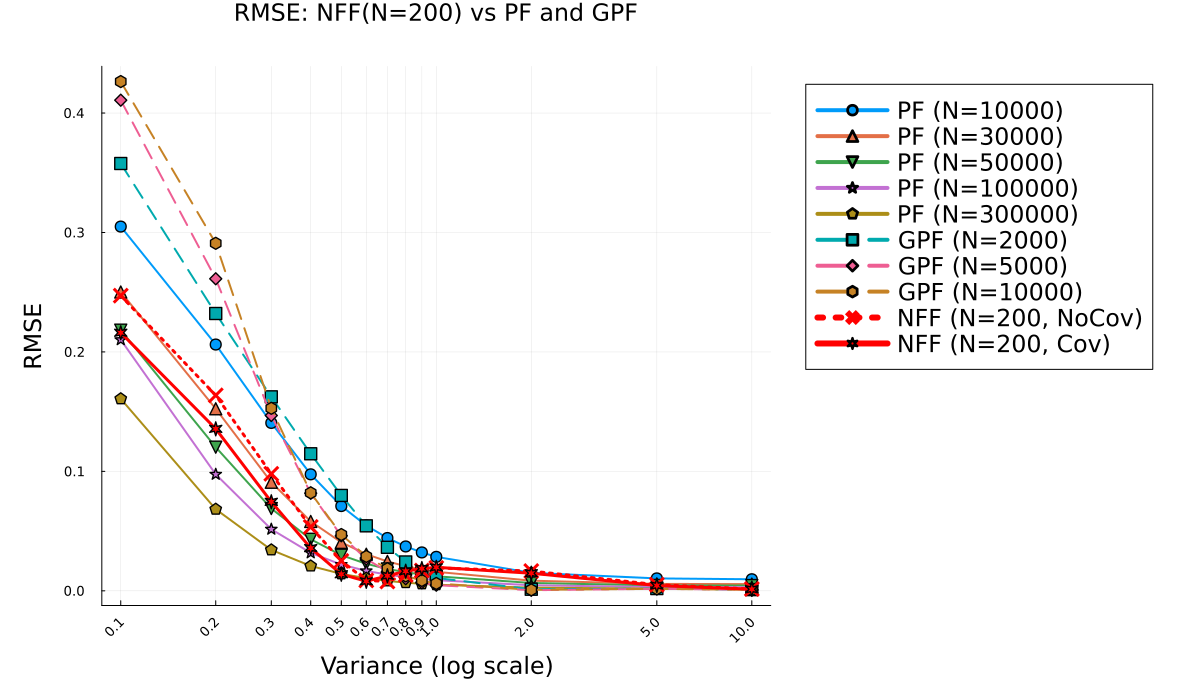
\includegraphics[width=\textwidth]{figures/Experiment01/rmse_NFF_CG_N200_vs_others.png}
		\caption{RMSE, $L=200$}
	\end{SubFigure}
	\hfill
	\begin{SubFigure}{0.48\textwidth}
		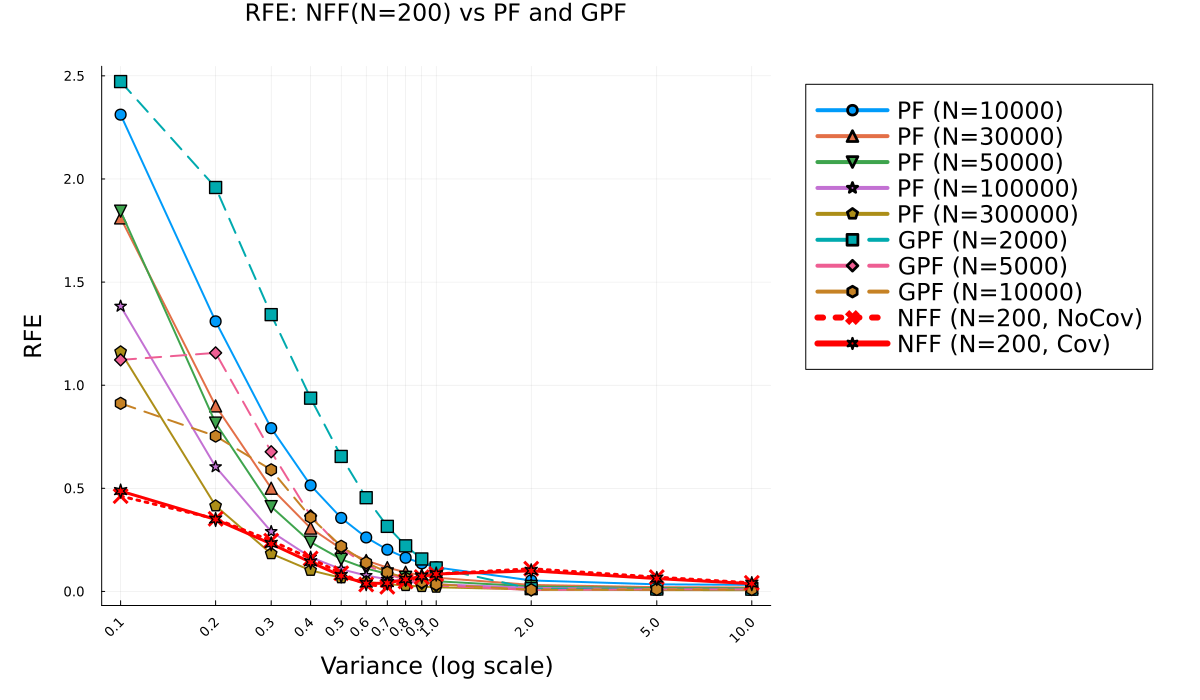
\includegraphics[width=\textwidth]{figures/Experiment01/rel_frob_NFF_CG_N200_vs_others.png}
		\caption{RFE, $L=200$}
	\end{SubFigure}
	
	\vspace{1em}
	
	% Row 2: L=500
	\begin{SubFigure}{0.48\textwidth}
		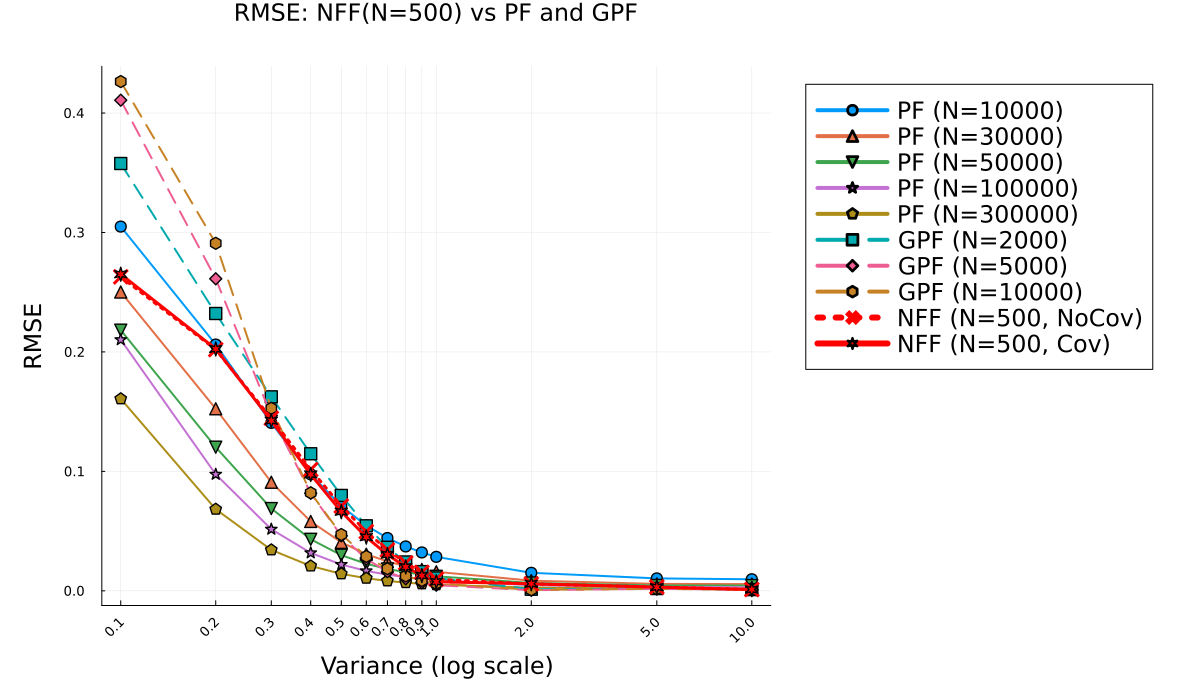
\includegraphics[width=\textwidth]{figures/Experiment01/rmse_NFF_CG_N500_vs_others.png}
		\caption{RMSE, $L=500$}
	\end{SubFigure}
	\hfill
	\begin{SubFigure}{0.48\textwidth}
		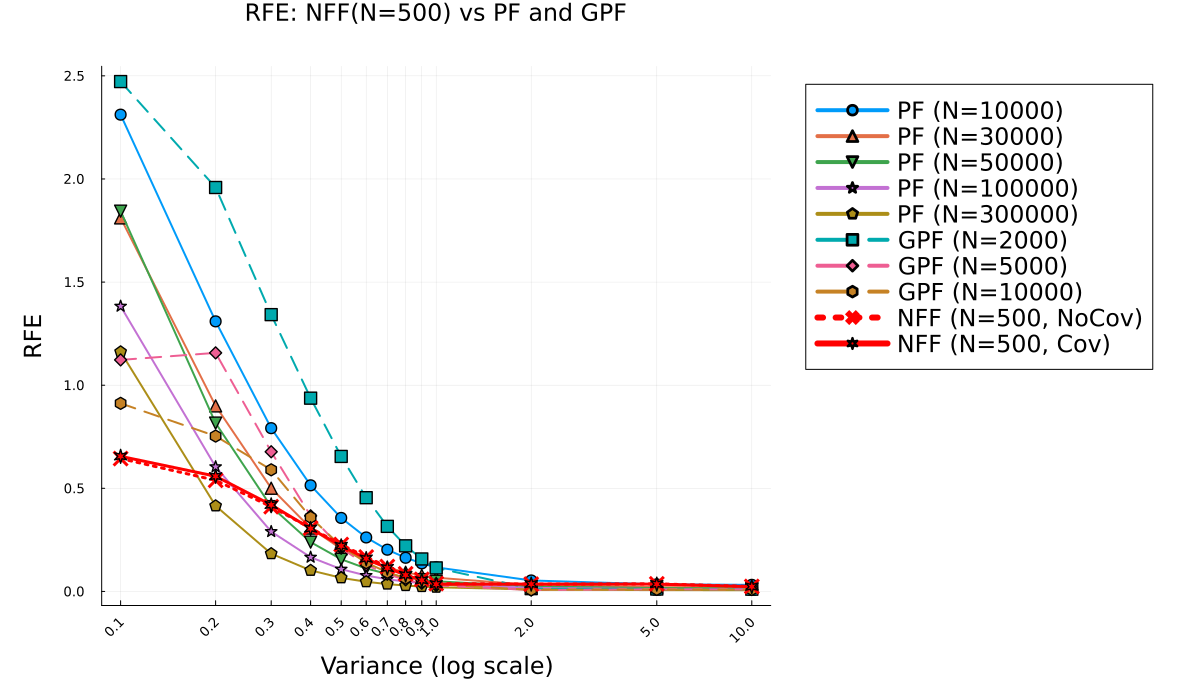
\includegraphics[width=\textwidth]{figures/Experiment01/rel_frob_NFF_CG_N500_vs_others.png}
		\caption{RFE, $L=500$}
	\end{SubFigure}
	
	\vspace{1em}
	
	% Row 3: L=1000
	\begin{SubFigure}{0.48\textwidth}
		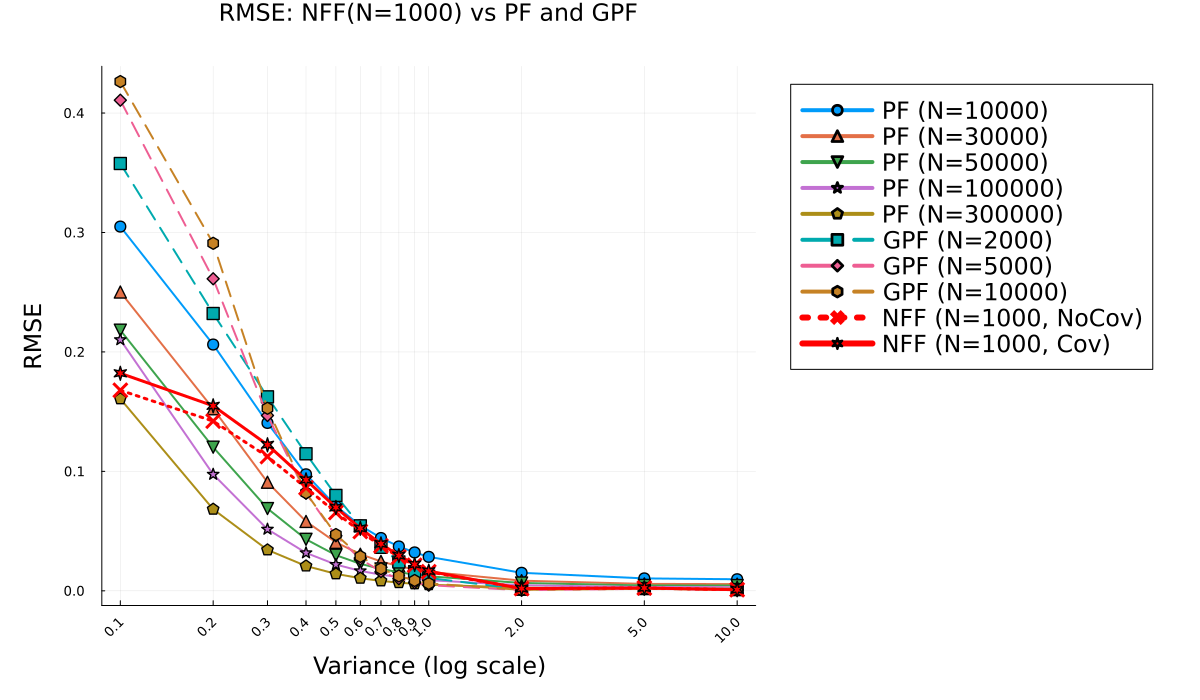
\includegraphics[width=\textwidth]{figures/Experiment01/rmse_NFF_CG_N1000_vs_others.png}
		\caption{RMSE, $L=1000$}
	\end{SubFigure}
	\hfill
	\begin{SubFigure}{0.48\textwidth}
		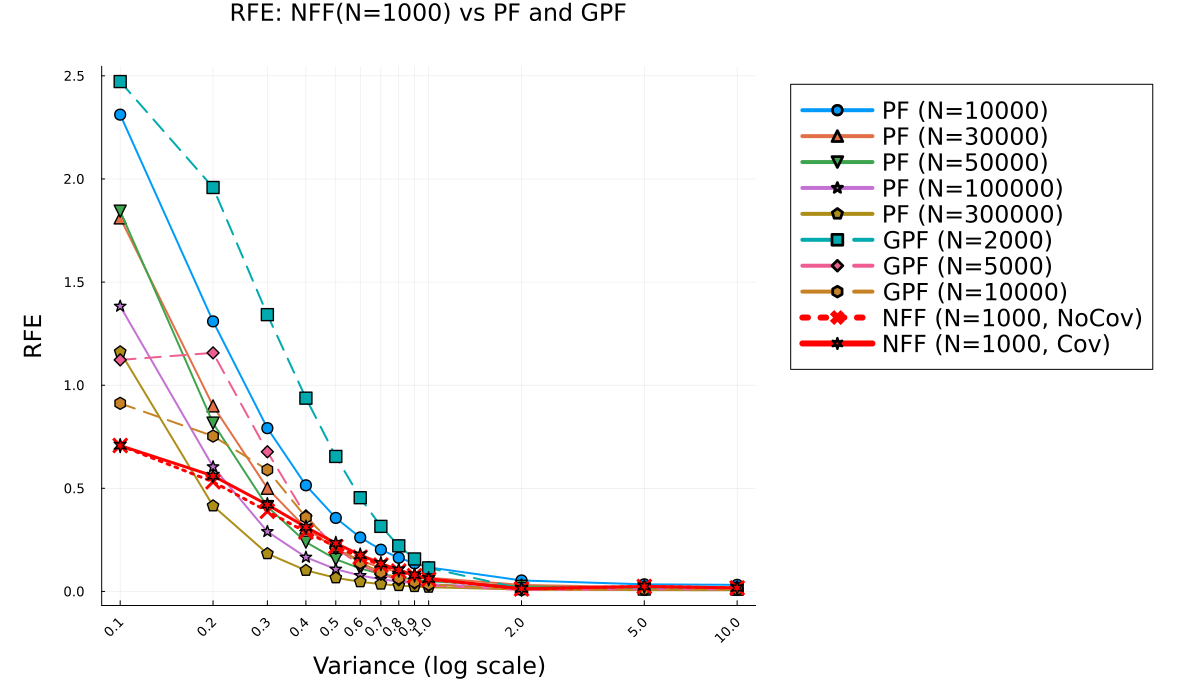
\includegraphics[width=\textwidth]{figures/Experiment01/rel_frob_NFF_CG_N1000_vs_others.png}
		\caption{RFE, $L=1000$}
	\end{SubFigure}
	
	\vspace{1em}
	
	% Row 4: L=2000
	\begin{SubFigure}{0.48\textwidth}
		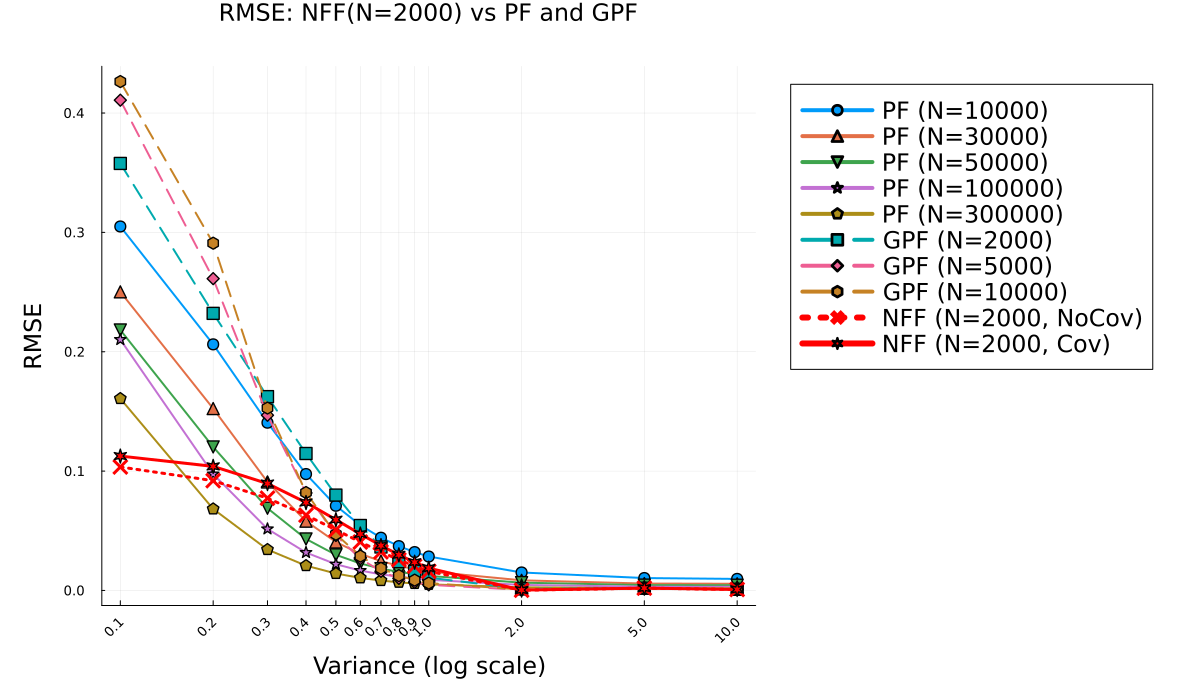
\includegraphics[width=\textwidth]{figures/Experiment01/rmse_NFF_CG_N2000_vs_others.png}
		\caption{RMSE, $L=2000$}
	\end{SubFigure}
	\hfill
	\begin{SubFigure}{0.48\textwidth}
		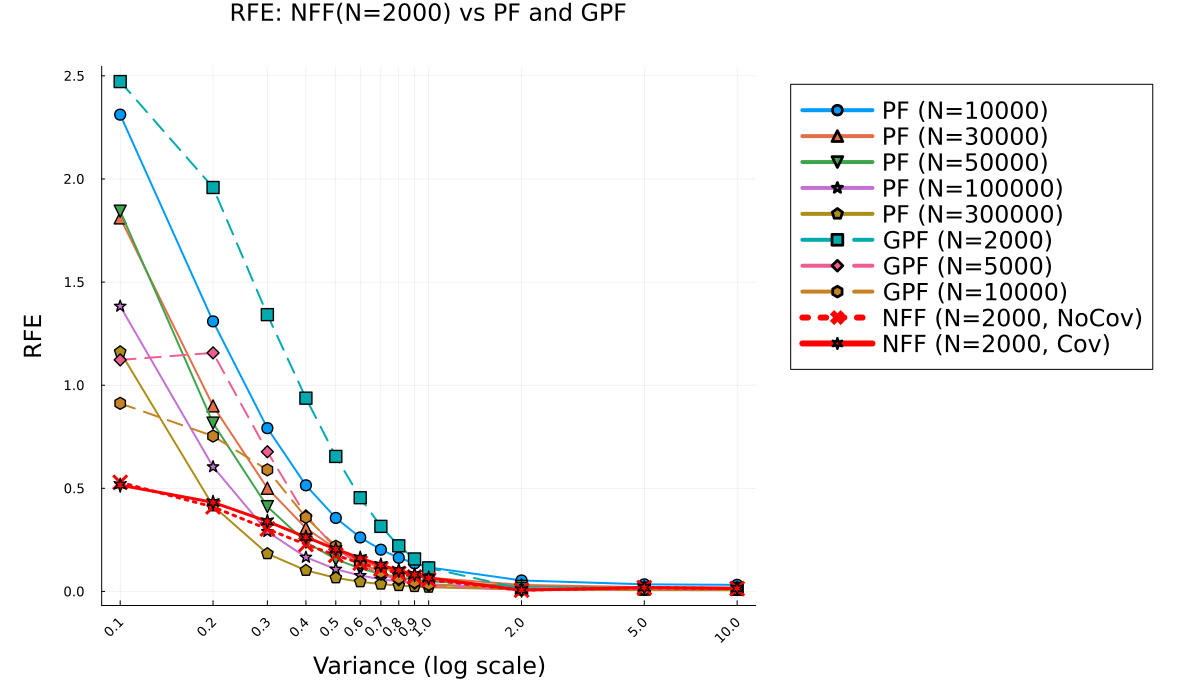
\includegraphics[width=\textwidth]{figures/Experiment01/rel_frob_NFF_CG_N2000_vs_others.png}
		\caption{RFE, $L=2000$}
	\end{SubFigure}
	
	\caption{RMSE and RFE vs. $\sigma_L^2$}
	\label{fig:likelihood_variance_results}
\end{Figure}

From \Fig{fig:likelihood_variance_results}, the following main conclusions can be drawn:

Regardless of the filtering algorithm, as the likelihood variance $\sigma_L^2$ decreases, both the mean estimation error and the covariance estimation error increase for all filters.

When the likelihood variance becomes very small, the covariance estimation errors of PF and GPF deteriorate rapidly. In contrast, the increase in the covariance estimation error of NFF is noticeably more gradual. In the likelihood variance range of $0.3 \sim 1.0$, the covariance estimation accuracy of NFF is comparable to that of PF with 50000 particles and GPF with 10000 particles. In the range $0.2 \sim 0.3$, NFF performs comparably to PF with 100000 to 300000 particles. When the likelihood variance becomes extremely small, in the range $0.1 \sim 0.2$, the covariance estimation accuracy of NFF even surpasses that of PF with 300000 particles.

With a relatively small number of particles (e.g., $L=200, 500$), the mean estimation accuracy of NFF, measured by RMSE, is comparable to that of PF with 10000 to 50000 particles. With a larger number of particles (e.g., $L=1000, 2000$), under extremely narrow likelihoods ($0.1 \sim 0.2$), the mean estimation accuracy of NFF also exceeds that of PF with 300000 particles. This indicates that the smaller the likelihood variance, the more pronounced the advantage of NFF becomes.

\subsection*{Why does a narrow likelihood lead to worse estimation results?}

For PF and GPF, the main cause of the error increase is severe particle degeneracy. When the likelihood variance is very small, the likelihood becomes sharply concentrated. In this case, most prior particles lie outside the effective support of the likelihood. During the update step, almost all particle weights approach zero. As a result, the number of effective particles drops sharply, and the filter loses its ability to approximate the posterior distribution.

For NFF, the error mainly arises from the sparsity of high-dimensional space and the information loss introduced during the approximation process. As the ODE drives the particles from the prior toward the posterior, the true posterior density is continuously approximated by an equal-weight particle representation. This process inevitably introduces information loss. Moreover, in a 10D state space, even 2000 particles remain highly sparse. When the likelihood is extremely sharp, its peak can easily fall into the large gaps between particles, which leads to additional information loss and less accurate estimates.

\subsection*{Why does a narrower likelihood increase the computation time of NFF?}

\begin{Figure}[ht]
	\centering
	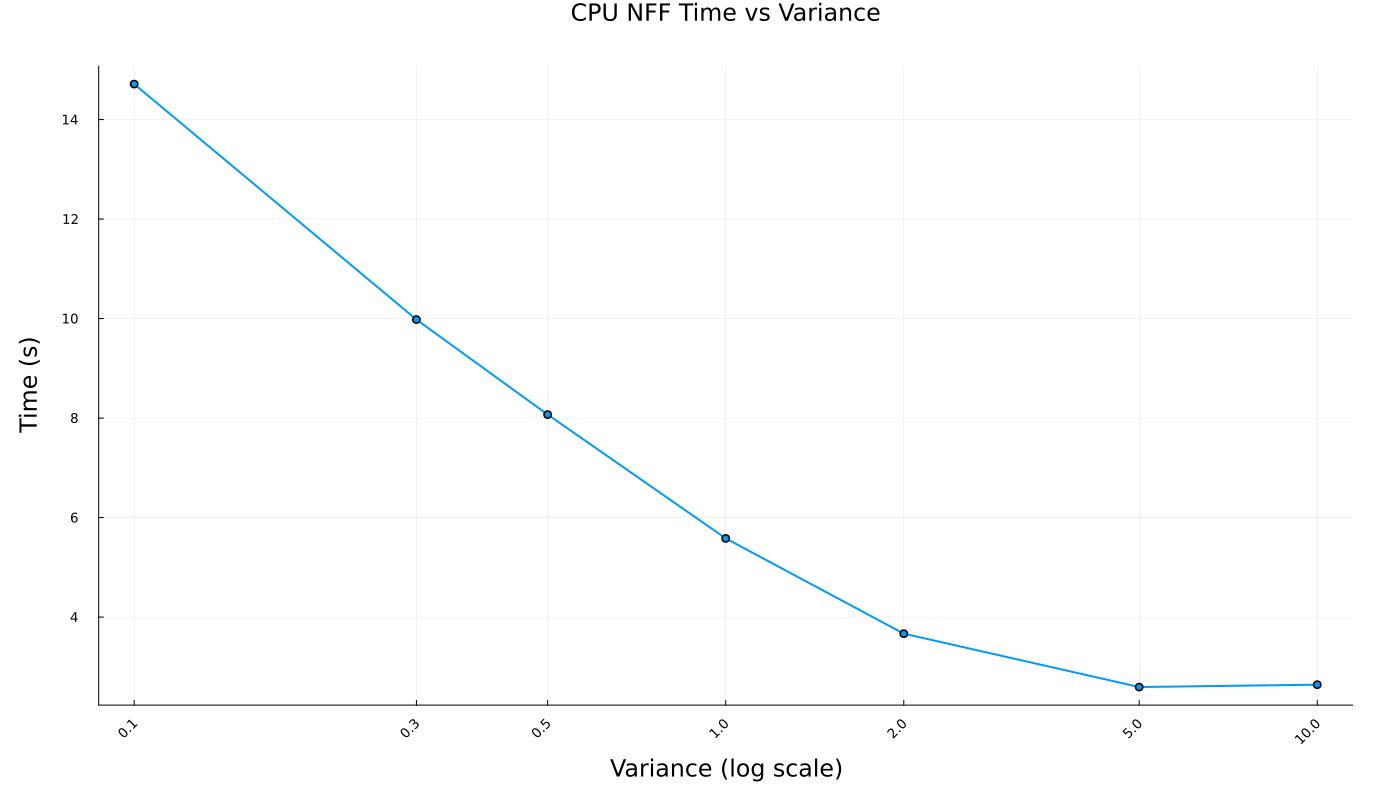
\includegraphics[width=0.9\textwidth]{figures/Experiment01/cpu_benchmark.png}
	\caption{CPU time vs. $\sigma_L^2$.}
	\label{fig:cpu_benchmark01}
\end{Figure}

As shown in \Fig{fig:cpu_benchmark01}, the single-step update time of NFF increases sharply as the likelihood variance decreases. As discussed in \SubSec{subsec:vcabm}, a narrower likelihood results in a stiffer ODE, which forces the VCABM integrator to take significantly more time to solve it.

\clearpage

\section{Prior-Likelihood Distance Sensitivity Analysis}
\label{sec:prior_likelihood_distance}

This experiment investigates the effect of the distance between the prior mean and the likelihood mean on the update accuracy of different filters. In this experiment, the likelihood covariance matrix is fixed at $\boldsymbol{\Sigma}_L = \mI_{10}$.

The control variable is the mean shift of the likelihood, with the likelihood mean $\vmu_L$ gradually increasing from 0.1 to 10.0. As this mean shift increases, the physical distance between the sensor observation region and the system prediction region also increases.

The RMSE and RFE of the filters under different mean shifts are shown in \Fig{fig:mean_shift_results}.

\begin{Figure}[ht]
	\centering
	% Row 1: L=200
	\begin{SubFigure}{0.48\textwidth}
		
\includegraphics[width=\textwidth]{figures/Experiment02/rmse_NFF_CG_N200_vs_others.png}
		\caption{RMSE, $L=200$}
		\label{fig:mean_shift_rmse_200}
	\end{SubFigure}
	\hfill
	\begin{SubFigure}{0.48\textwidth}
		
\includegraphics[width=\textwidth]{figures/Experiment02/rel_frob_NFF_CG_N200_vs_others.png}
		\caption{Rel. Frobenius Error, $L=200$}
		\label{fig:mean_shift_frob_200}
	\end{SubFigure}
	
	\vspace{1em}
	
	% Row 2: L=500
	\begin{SubFigure}{0.48\textwidth}
		
\includegraphics[width=\textwidth]{figures/Experiment02/rmse_NFF_CG_N500_vs_others.png}
		\caption{RMSE, $L=500$}
		\label{fig:mean_shift_rmse_500}
	\end{SubFigure}
	\hfill
	\begin{SubFigure}{0.48\textwidth}
		
\includegraphics[width=\textwidth]{figures/Experiment02/rel_frob_NFF_CG_N500_vs_others.png}
		\caption{Rel. Frobenius Error, $L=500$}
		\label{fig:mean_shift_frob_500}
	\end{SubFigure}
	
	\vspace{1em}
	
	% Row 3: L=1000
	\begin{SubFigure}{0.48\textwidth}
		
\includegraphics[width=\textwidth]{figures/Experiment02/rmse_NFF_CG_N1000_vs_others.png}
		\caption{RMSE, $L=1000$}
		\label{fig:mean_shift_rmse_1000}
	\end{SubFigure}
	\hfill
	\begin{SubFigure}{0.48\textwidth}
		
\includegraphics[width=\textwidth]{figures/Experiment02/rel_frob_NFF_CG_N1000_vs_others.png}
		\caption{Rel. Frobenius Error, $L=1000$}
		\label{fig:mean_shift_frob_1000}
	\end{SubFigure}
	
	\vspace{1em}
	
	% Row 4: L=2000
	\begin{SubFigure}{0.48\textwidth}
		
\includegraphics[width=\textwidth]{figures/Experiment02/rmse_NFF_CG_N2000_vs_others.png}
		\caption{RMSE, $L=2000$}
		\label{fig:mean_shift_rmse_2000}
	\end{SubFigure}
	\hfill
	\begin{SubFigure}{0.48\textwidth}
		
\includegraphics[width=\textwidth]{figures/Experiment02/rel_frob_NFF_CG_N2000_vs_others.png}
		\caption{Rel. Frobenius Error, $L=2000$}
		\label{fig:mean_shift_frob_2000}
	\end{SubFigure}
	
	\caption{RMSE and RFE vs. likelihood mean.}
	\label{fig:mean_shift_results}
\end{Figure}

From \Fig{fig:mean_shift_results}, the following main conclusions can be drawn:

As the likelihood distribution moves farther away from the prior distribution, both the mean estimation error and the covariance estimation error increase across all filtering algorithms.

When the likelihood mean shift lies in the large-deviation range from 1.5 to 10.0, the RMSE and RFE of PF and GPF increase dramatically, and these filters effectively fail. In contrast, the error of NFF remains at a very low level. This indicates that the farther the likelihood is from the prior, the more pronounced the advantage of NFF becomes.

\subsection*{Why do more distant likelihoods lead to less accurate estimates?}

PF and GPF fail under distant likelihoods because they suffer from severe particle degeneracy.

For NFF, as discussed earlier, the particle flow continuously replaces the true posterior density by an approximate posterior density. This repeated approximation inevitably introduces information loss throughout the flow process.

\subsection*{Why does a more distant likelihood increase the computation time of NFF?}

\begin{Figure}[ht]
	\centering
	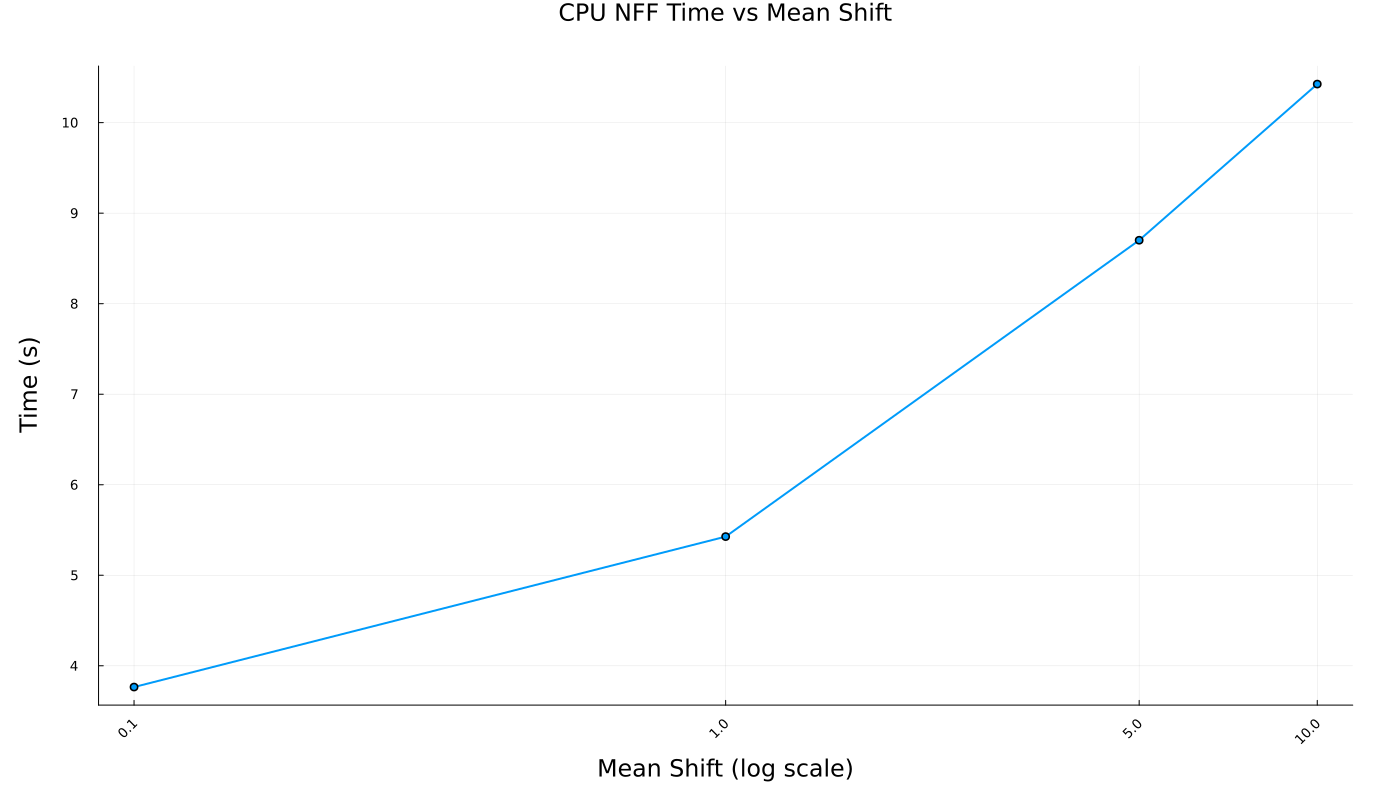
\includegraphics[width=0.9\textwidth]{figures/Experiment02/time_benchmark.png}
	\caption{CPU update time vs. likelihood mean.}
	\label{fig:cpu_benchmark02}
\end{Figure}

This correlation between the likelihood mean and the computational cost is demonstrated in \Fig{fig:cpu_benchmark02}. As discussed earlier in \SubSec{subsec:vcabm}, when the initial particle cloud is very far from the effective support of the likelihood, the ODE becomes highly stiff. As a result, the VCABM integrator must use much smaller step sizes to maintain accuracy, which significantly increases the total computation time.

\clearpage

\section{Influence of State Dimension}
\label{sec:influence_dimension}

To investigate how the state dimension affects filtering accuracy, this experiment uses the state dimension $N$ as the control variable and increases it gradually from 2 to 20.

In these experiments, the prior and likelihood parameters are fixed. The likelihood covariance is set to $\boldsymbol{\Sigma}_L = 0.3 \mI_N$, and the mean in each dimension is fixed at 5, such that $\vmu_L = [5, 5, \dots, 5]^{\top}$.

When comparing mean estimation accuracy across different dimensions, RMSE is not an appropriate metric. This is because as the dimension $N$ increases, the norm of the true posterior mean vector $\vmu_\text{true}$ also increases naturally. To remove this scaling effect, this experiment uses the Relative Mean Error (RME) as the main metric given by
\begin{equation}
	\text{RME} = \frac{||\hat{\vx} - \vmu_\text{true}||}{||\vmu_\text{true}||} \enspace .
\end{equation}
RME provides a dimensionless benchmark for comparing performance across different state dimensions.

The RME and RFE of the filters under different state dimensions are shown in \Fig{fig:dimension_results}.

\begin{Figure}[ht]
	\centering
	\begin{SubFigure}{0.48\textwidth}
		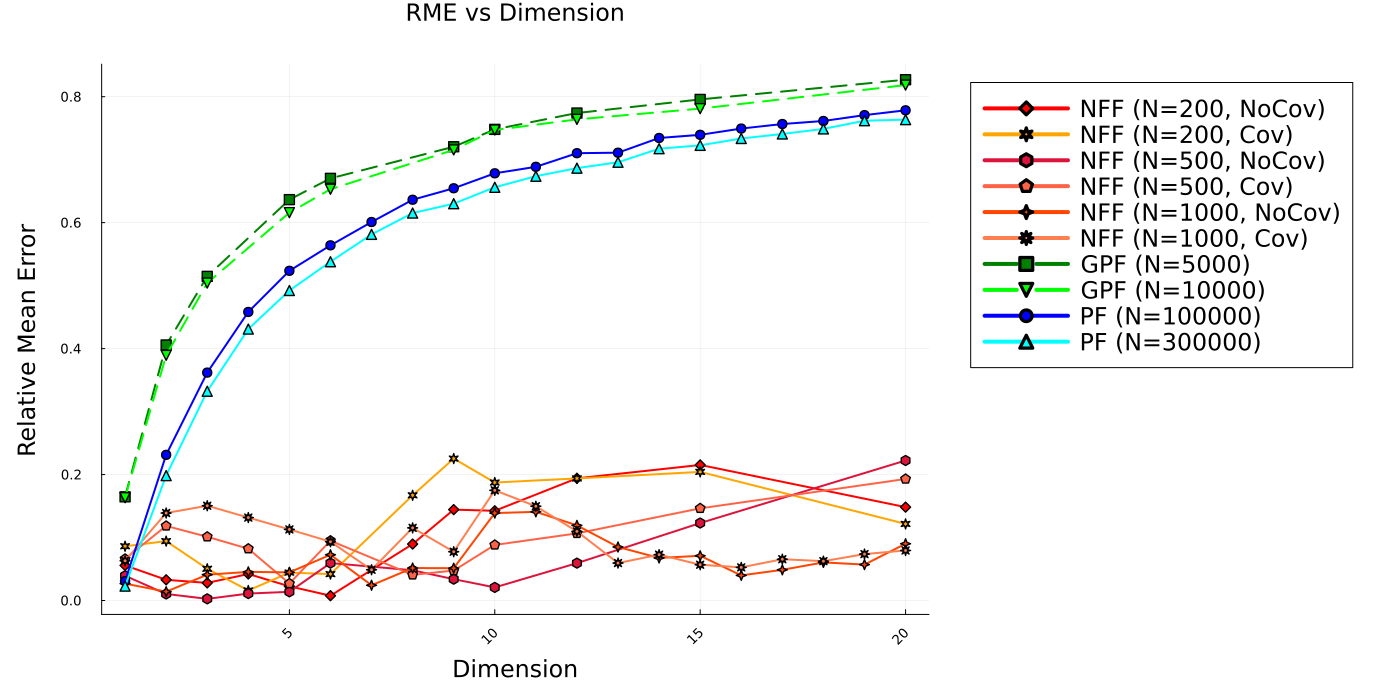
\includegraphics[width=\textwidth]{figures/Experiment04/e_mu.png}
		\caption{RME vs. Dimension.}
		\label{fig:rme_vs_dim}
	\end{SubFigure}
	\hfill
	\begin{SubFigure}{0.48\textwidth}
		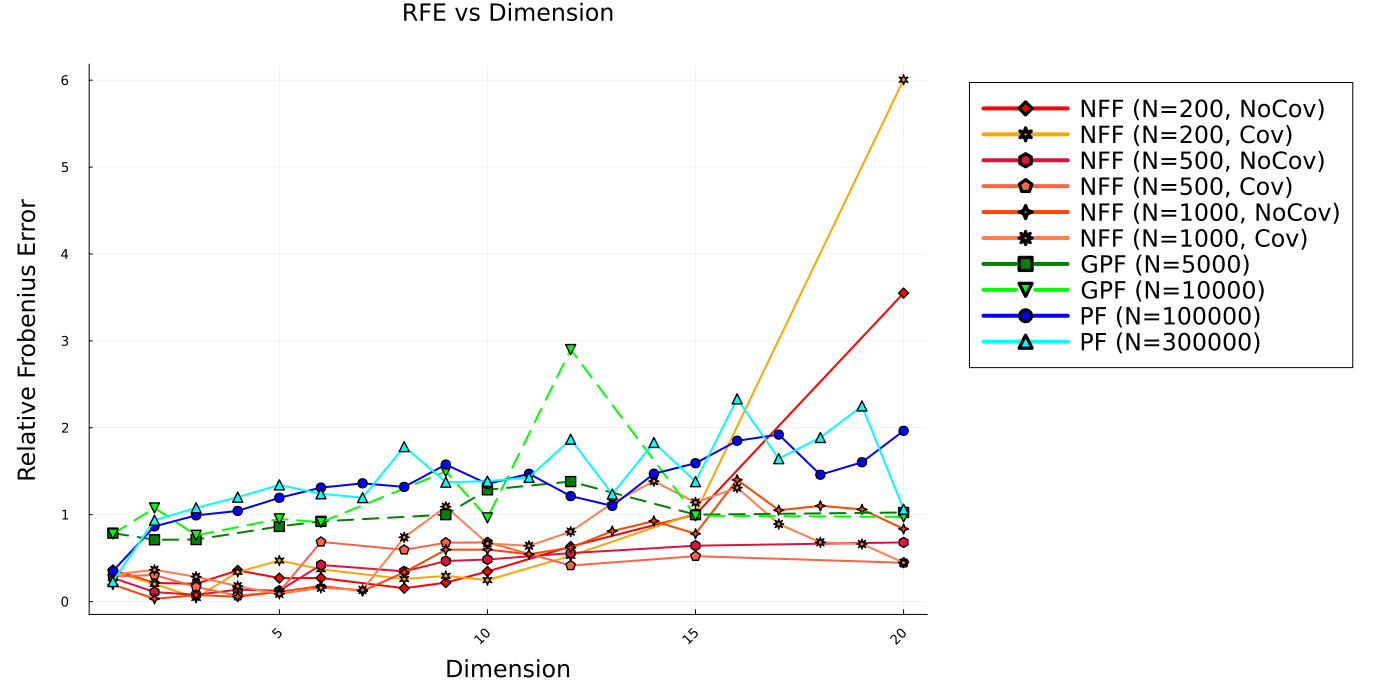
\includegraphics[width=\textwidth]{figures/Experiment04/rel_frob.png}
		\caption{RFE vs. Dimension.}
		\label{fig:frob_vs_dim}
	\end{SubFigure}
	\caption{RME and RFE vs. dimension.}
	\label{fig:dimension_results}
\end{Figure}

The following conclusions can be drawn:

Within the tested range from 2 to 20 dimensions, the mean estimation accuracy of PF and GPF deteriorates rapidly as the dimension increases. At 20 dimensions, their RME exceeds 0.8, indicating that the filters have essentially lost track of the target. In contrast, the RME of NFF changes only slightly and remains stable below 0.2.

When the state dimension satisfies $N \in [2, 15]$, the RFE of NFF remains below 1.0, and its covariance estimation accuracy is better than that of PF with 300000 particles. When the dimension increases further from 15 to 20, the relative Frobenius error of NFF with 200 or 500 particles rises sharply because of the limited particle number. However, the covariance estimation accuracy of NFF with 1000 particles is still comparable to that of GPF with 10000 particles and remains better than that of PF. Compared with PF and GPF, NFF is therefore better suited to state estimation in high-dimensional spaces.

\clearpage

\section{Parameter Analysis of NFF}
\label{sec:parameter_analysis}

This section presents a sensitivity analysis of the internal parameters of NFF under a baseline scenario in which the prior is a standard normal distribution, the likelihood mean is fixed at $\vmu_L = [5, 5, \dots, 5]^{\top}$, and the likelihood covariance is fixed at $\boldsymbol{\Sigma}_L = 0.3 \mI_{10}$.

\subsection{Influence of Particle Count}
\label{subsec:particle_count_impact}

This experiment evaluates the performance of NFF for different particle counts ($L \in [100, 2000]$) and compares the resulting errors with those of PF and GPF. The results are shown in \Fig{fig:nff_parameter_L}.

\begin{Figure}[ht]
	\centering
	\begin{SubFigure}{\textwidth}
		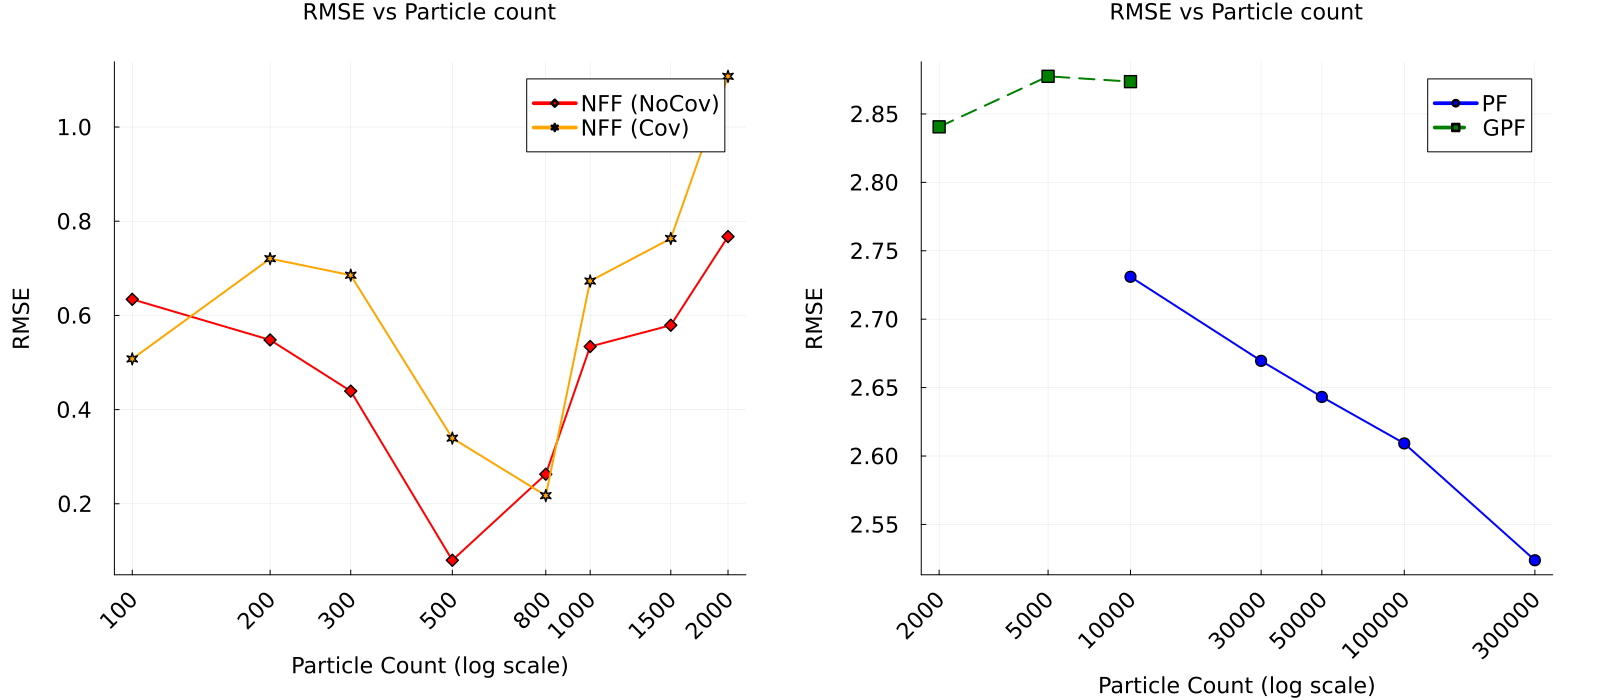
\includegraphics[width=\textwidth]{figures/Experiment3.1/rmse.png}
		\caption{RMSE vs. particle count $L$.}
		\label{fig:nff_rmse_L}
	\end{SubFigure}
	
	\vspace{1.5em}
	
	\begin{SubFigure}{\textwidth}
		
\includegraphics[width=\textwidth]{figures/Experiment3.1/rel_frob.png}
		\caption{RFE vs. particle count $L$.}
		\label{fig:nff_frob_L}
	\end{SubFigure}
	
	\caption{RMSE and RFE vs. particle count $L$}
	\label{fig:nff_parameter_L}
\end{Figure}

\textbf{U-shaped trend in mean estimation error:} As shown in the results, unlike standard particle filters, for which a larger number of particles usually improves mean estimation accuracy, the mean estimation error of NFF exhibits a U-shaped trend as the particle count increases. This indicates that, for NFF mean estimation, more particles are not always beneficial.

When the number of particles is too small (e.g., 100--200), the particle distribution is too sparse in the 10D state space to approximate the true posterior effectively, which leads to a large mean estimation error. However, when the number of particles becomes too large (e.g., 1000--2000), the cross terms in the modified Cramér--von Mises distance \Eq{eq:CVM_Dxy} become extremely numerous and complex. The increasing contribution of these cross terms weakens the relative influence of the mean-difference term ($D_E$) in the optimization objective. As a result, the algorithm must operate in a balanced particle range, such as 300--500 particles in the present scenario, which is sufficiently dense to approximate the distribution while avoiding excessive cross-term complexity.

Regarding covariance estimation, the relative Frobenius error shows that the accuracy is poor when the particle count is small. The error decreases rapidly and reaches its minimum when the particle count is around 300. Beyond this point, although the covariance error fluctuates slightly as more particles are added, it remains within a reasonable range, stays below 1.0, and performs significantly better than PF.

\textbf{Constraint comparison:} Comparing NFF with and without covariance constraints shows that, in the present scenario, the constrained version is actually less accurate in estimating both the mean and the covariance than the unconstrained version. This disadvantage is especially pronounced when the number of particles is large.

NFF with covariance constraints adds the second-moment penalty term \Eq{eq:D_Cov} to the CVM optimization objective. In order to reduce the discrepancy in the second moment, the algorithm must compromise on the optimization of the first moment and the higher-order distribution structure represented by the kernel cross terms. This multi-objective trade-off leads to a reduction in overall estimation accuracy when covariance constraints are imposed.
\clearpage

\subsection{Selection of the Homotopy Function}
\label{subsec:homotopy_function_selection}

In NFF, the homotopy function must satisfy the boundary conditions $g(0)=0$ and $g(1)=1$, but its path within the interval $\gamma \in (0, 1)$ can be chosen freely. To investigate how the shape of the homotopy function affects filtering accuracy and computational efficiency, this section compares five different homotopy functions and their corresponding derivatives $\dot{g}(\gamma)$.

The tested functions include a linear function $g(\gamma) = \gamma$ with derivative $\dot{g}(\gamma) = 1.0$, and a convex function $g(\gamma) = \gamma^2$ with derivative $\dot{g}(\gamma) = 2\gamma$. In addition, a concave function $g(\gamma) = -\gamma^2 + 2\gamma$ with derivative $\dot{g}(\gamma) = -2\gamma + 2$ is evaluated. More complex paths are also considered, including a convex-then-concave function
$g(\gamma) = \frac{1}{2}\sin(\pi\gamma - \frac{\pi}{2}) + \frac{1}{2}$
with derivative
$\dot{g}(\gamma) = \frac{\pi}{2}\cos(\pi\gamma - \frac{\pi}{2})$,
and a concave-then-convex function
$g(\gamma) = \gamma^3 - \frac{3}{2}\gamma^2 + \frac{3}{2}\gamma$
with derivative
$\dot{g}(\gamma) = 3\gamma^2 - 3\gamma + 1.5$. These homotopy functions and their corresponding derivatives are illustrated in \Fig{fig:function_plots}.

\begin{Figure}[ht]
    \centering
    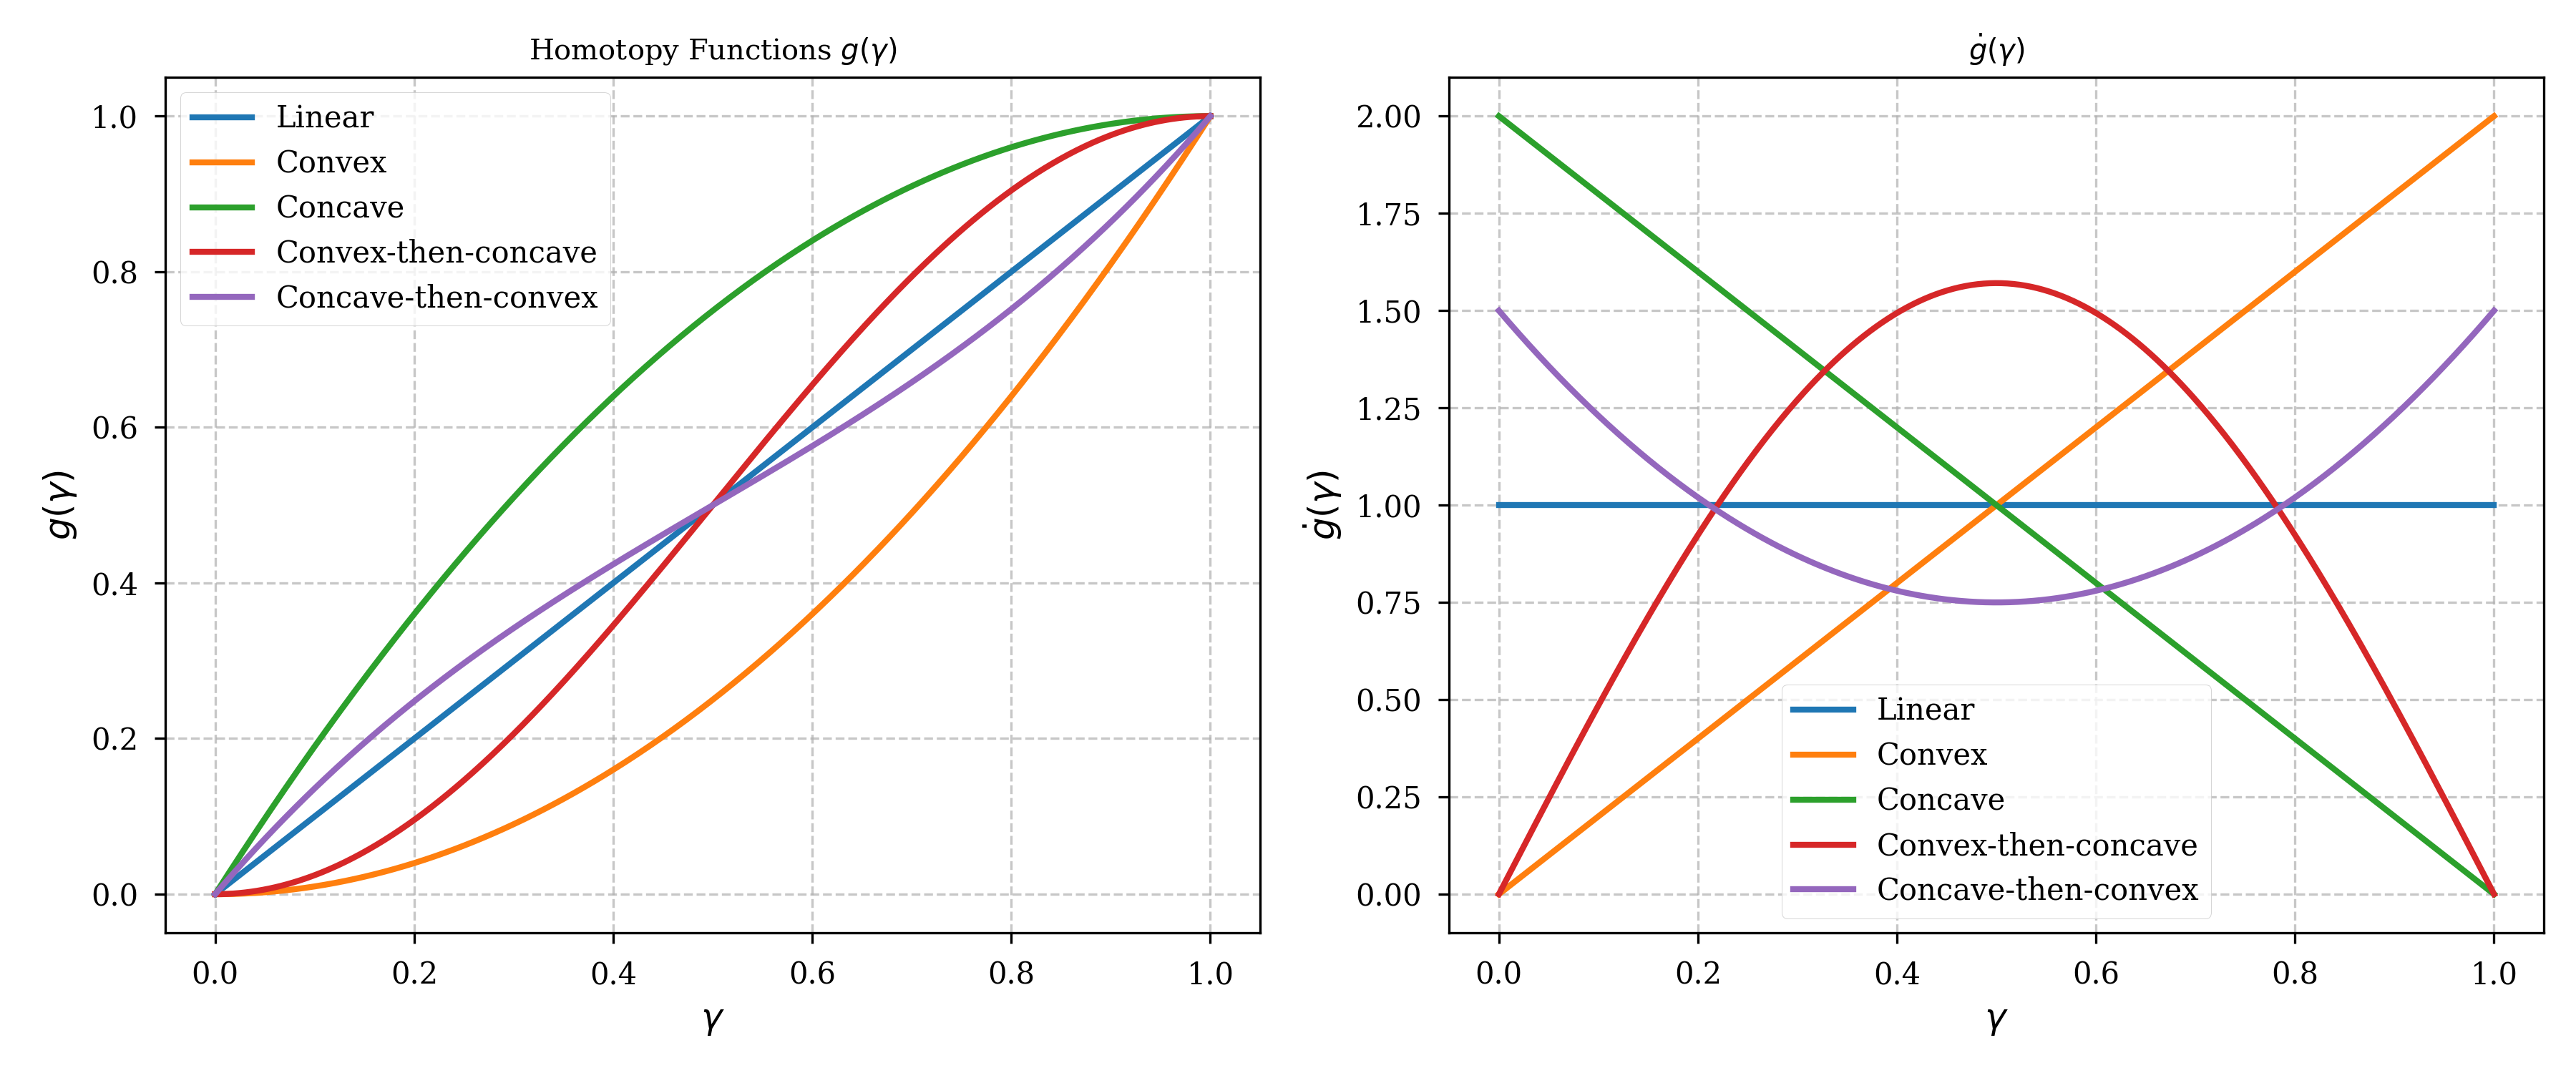
\includegraphics[width=0.95\textwidth]{figures/homotopy_function.png} 
    \caption{Comparison of homotopy functions $g(\gamma)$ and their derivatives $\dot{g}(\gamma)$.}
    \label{fig:function_plots}
\end{Figure}

The experimental results are shown in \Fig{fig:homotopy_results}.

\begin{Figure}[ht]
	\centering
	\begin{SubFigure}{0.48\textwidth}
		\centering
		
\includegraphics[width=\textwidth]{figures/Experiment3.2/rmse.png}
		\caption{RMSE vs. $g(\gamma)$}
		\label{fig:homotopy_rmse}
	\end{SubFigure}
	\hfill
	\begin{SubFigure}{0.48\textwidth}
		\centering
		
\includegraphics[width=\textwidth]{figures/Experiment3.2/rel_frob.png}
		\caption{RFE vs. $g(\gamma)$}
		\label{fig:homotopy_frob}
	\end{SubFigure}
	
	\vspace{1em}
	\begin{SubFigure}{0.48\textwidth}
		\centering
		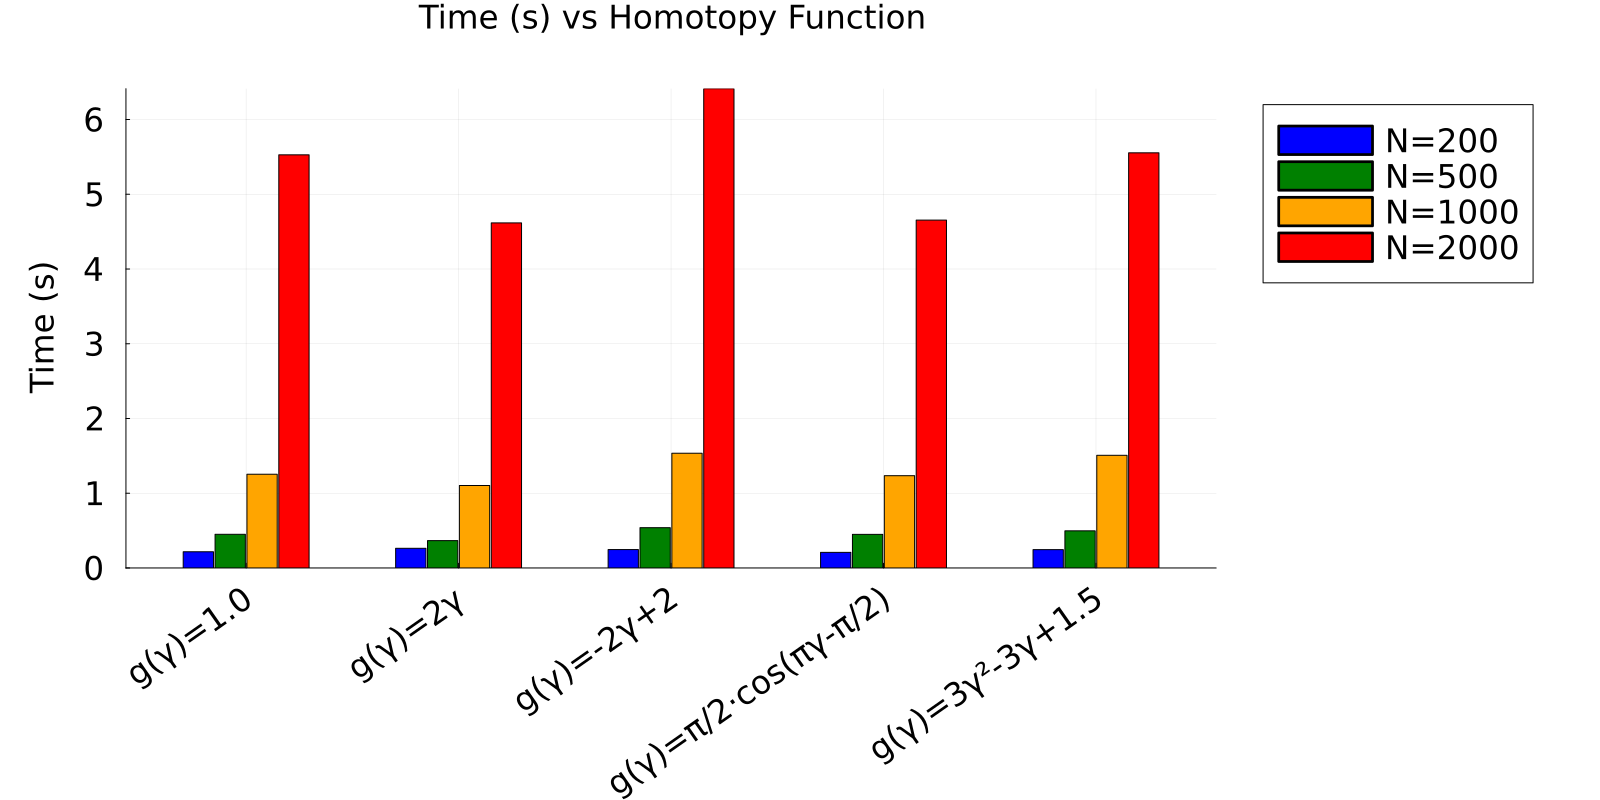
\includegraphics[width=\textwidth]{figures/Experiment3.2/time.png}
		\caption{Computation time vs. $g(\gamma)$}
		\label{fig:homotopy_time}
	\end{SubFigure}
	
	\caption{Accuracy and efficiency vs. $g(\gamma)$.}
	\label{fig:homotopy_results}
\end{Figure}

The bar charts for RMSE and RFE show that, under the same particle configuration, the mean and covariance estimation accuracy is almost identical for all five functions. This indicates that the absolute accuracy of the filter is largely insensitive to the specific shape of the homotopy path.

However, the computation-time plot clearly shows that different homotopy functions lead to noticeable differences in computational cost. In particular, the execution time is substantially reduced when the convex function ($\dot{g}(\gamma)=2\gamma$) or the convex-then-concave function ($\dot{g}(\gamma) = \frac{\pi}{2}\cos(\pi\gamma - \frac{\pi}{2})$) is used. In contrast, the execution time increases significantly for the concave and concave-then-convex functions.

The root cause of these timing differences is that the derivative $\dot{g}(\gamma)$ directly controls the initial stiffness of the ODE. As shown in the previous derivation, during the initial stage of the virtual-time evolution ($\gamma \to 0$), the particle set is still located in the prior region, which is far from the high-probability region of the likelihood and therefore produces a stiff ODE system. If a concave homotopy is used, for example with $\dot{g}(0) = 2$, the stiffness becomes even stronger. By contrast, when a convex or convex-then-concave homotopy is used, with $\dot{g}(0) = 0$, the derivative is initially very small. This small numerical multiplier alleviates the stiffness caused by the large initial distance between the particles and the likelihood region.

Therefore, in practical applications of NFF, a convex or convex-then-concave homotopy function should be preferred. This choice preserves the original estimation accuracy while mitigating the initial stiffness of the ODE, thereby significantly improving computational efficiency.
\clearpage

\subsection{Influence of the Regularization Parameter}
\label{subsec:regularization_parameter}

In the theoretical derivation of NFF, a small regularization parameter $d_{\min}^2$ is introduced to avoid numerical problems when the inter-particle distance approaches zero. To investigate the effect of this parameter, four values of $d_{\min}^2$ with different orders of magnitude ($10^{-24}, 10^{-16}, 10^{-8}, 10^{-3}$) are compared. The results are shown in \Fig{fig:regularization_results}.

\begin{Figure}[ht]
	\centering
	\begin{SubFigure}{0.48\textwidth}
		\centering
		
\includegraphics[width=\textwidth]{figures/Experiment3.3/rmse.png}
		\caption{RMSE vs. $d_{\min}^2$.}
		\label{fig:dmin_rmse}
	\end{SubFigure}
	\hfill
	\begin{SubFigure}{0.48\textwidth}
		\centering
		
\includegraphics[width=\textwidth]{figures/Experiment3.3/rel_frob.png}
		\caption{RFE vs. $d_{\min}^2$.}
		\label{fig:dmin_frob}
	\end{SubFigure}
	
	\vspace{1em}
	
	\begin{SubFigure}{0.48\textwidth}
		\centering
		
\includegraphics[width=\textwidth]{figures/Experiment3.3/time.png}
		\caption{Computation time vs. $d_{\min}^2$.}
		\label{fig:dmin_time}
	\end{SubFigure}
	
	\caption{Accuracy and efficiency vs. $d_{\min}^2$.}
	\label{fig:regularization_results}
\end{Figure}

As shown in the results, both RMSE and RFE worsen as $d_{\min}^2$ increases. In addition, the single-step update time of the algorithm increases significantly with larger values of $d_{\min}^2$.
\clearpage

\subsection{Influence of the Penalty Coefficient}
\label{subsec:penalty_coefficient}

In the CVM distance, the coefficient $K$ acts as a first-moment penalty coefficient. It controls the weight assigned to the mean difference between the two distributions in the total optimization objective. To analyze the effect of this parameter, the experiment evaluates several values of $K$ with different magnitudes.

\begin{Figure}[ht]
	\centering
	\begin{SubFigure}{0.48\textwidth}
		\centering
		
\includegraphics[width=\textwidth]{figures/Experiment3.4/rmse.png}
		\caption{RMSE vs. $K$.}
		\label{fig:penalty_rmse}
	\end{SubFigure}
	\hfill
	\begin{SubFigure}{0.48\textwidth}
		\centering
		
\includegraphics[width=\textwidth]{figures/Experiment3.4/rel_frob.png}
		\caption{RFE vs. $K$.}
		\label{fig:penalty_frob}
	\end{SubFigure}
	
	\caption{RMSE and RFE vs. $K$.}
	\label{fig:penalty_K_results}
\end{Figure}

The results(\Fig{fig:penalty_K_results}) show that as the penalty coefficient $K$ increases, the covariance estimation accuracy of NFF gradually deteriorates. However, once $K$ reaches a sufficiently large value (e.g., $K \ge 100$), the mean estimation error decreases and remains at a highly accurate level.
\clearpage

\section{Limitations in Handling Multimodal Distributions}
\label{sec:multimodal_limitations}

The analysis is carried out in a 10-dimensional state space. The prior distribution is fixed as a standard normal distribution $\Gaussian(\vzero, \mI_{10})$. The likelihood is defined as a bimodal Gaussian mixture with two equally weighted components. The covariance matrices of both modes are fixed at $0.3\mI_{10}$, and their means are located at two distinct points in space:
$\vmu_1 = [5, 5, \dots, 5]^{\top}$ and $\vmu_2 = [-5, -5, \dots, -5]^{\top}$.

\begin{table}[ht]
	\footnotesize
	\setlength{\tabcolsep}{3pt}
	
	\begin{tabularx}{\textwidth}{|X|c|c|c|c|c|c|}
		\hline
		\textbf{Filter} & \textbf{M1 RMSE} & \textbf{M1 RelFrob} & \textbf{M2 RMSE} & \textbf{M2 RelFrob} & \textbf{M1 Count} & \textbf{M2 Count} \\ \hline
		\makecell[l]{NFF\\($L=200$)} & 0.9402 & 0.4778 & N/A & N/A & 200 & 0 \\ \hline
		\makecell[l]{NFF Cov\\($L=200$)} & N/A & N/A & 1.1158 & 0.8741 & 0 & 200 \\ \hline
		\makecell[l]{NFF\\($L=500$)} & N/A & N/A & 1.1046 & 0.4390 & 0 & 500 \\ \hline
		\makecell[l]{NFF Cov\\($L=500$)} & 1.0810 & 0.8291 & N/A & N/A & 500 & 0 \\ \hline
		\makecell[l]{NFF\\($L=1000$)} & 0.9945 & 1.6006 & N/A & N/A & 1000 & 0 \\ \hline
		\makecell[l]{NFF Cov\\($L=1000$)} & 1.4922 & 0.9810 & N/A & N/A & 1000 & 0 \\ \hline
		\makecell[l]{NFF\\($L=2000$)} & 0.9429 & 5.7725 & N/A & N/A & 2000 & 0 \\ \hline
		\makecell[l]{NFF Cov\\($L=2000$)} & 1.0327 & 0.9259 & N/A & N/A & 2000 & 0 \\ \hline
		GPF & 2.8736 & 0.9627 & 2.8069 & 0.9930 & 5002 & 4998 \\ \hline
		PF (avg. 30 runs) & 2.5238 & 1.3845 & 2.5078 & 1.5309 & 149970 & 150030 \\ \hline
	\end{tabularx}
	\caption{Bimodal tracking results: NFF vs. GPF and PF.}
	\label{tab:multimodal_results}
\end{table}

After the update step of NFF, a hyperplane defined by $\sum \vx_i = 0$ is used as a classification boundary to count the particle distribution across the two modes. Particles whose coordinate sum is greater than zero are classified as having moved toward the first mode ($\vmu_1$), whereas particles whose coordinate sum is less than zero are classified as having moved toward the second mode ($\vmu_2$).

In the 10-dimensional bimodal fusion experiment, the particle set of NFF consistently flows as a whole toward only one of the two likelihood modes after the update step is completed. No particles are assigned to the other symmetric mode. This phenomenon is clearly evident from the particle counts recorded in \Tab{tab:multimodal_results}.
\clearpage
	\chapter{Comparative Experiments in the Lorenz 96 System}
\label{chap:lorenz96_experiments}

This chapter evaluates the performance of NFF in the Lorenz 96 system and compares it with PF and GPF. PF employs systematic resampling. Because particle degeneracy occurs easily in a 10-dimensional state space, the number of PF particles is increased to 5000, 10000, 30000, and 50000 to ensure filter stability. GPF uses the LCD-based deterministic sampling strategy, with particle counts of 2000, 5000, and 10000. For NFF, the particle counts are set to 500, 1000, and 2000. In the prediction step of NFF, Method 1 and Method 3 proposed in Chapter 3 are tested, and both the covariance-constrained (C) and unconstrained (NC) variants are evaluated.

The system is configured with state dimension $N=10$ and forcing parameter $F=8.0$. The discretization time step is set to $\Delta t=0.1$. All tests are conducted under the same initial uncertainty to ensure a fair comparison. To obtain statistically meaningful results, PF and GPF are evaluated over 20 independent Monte Carlo random seeds, whereas NFF is evaluated over 5 seeds. For each seed, the filtering process is run continuously for 100 time steps.

The source code for these experiments is available in \cite{Code_MA25_Wang}. This project relies on the libraries and implementations provided in \cite{Code_Filters_JL, Code_LCD_numeric, Code_DetGaussSampling}.

\section{Sensitivity to Noise Environments}
\label{sec:noise_sensitivity}

\subsection{Measurement Noise}
\label{subsec:measurement_noise}

This experiment evaluates the performance of different filters under different observation precisions. The intensity of the system process noise is fixed at 1, which, after discretization, corresponds to a cumulative process noise per step following a Gaussian distribution with variance 0.1. The control variable is the measurement noise variance, which is set to the sequence [0.01, 0.05, 0.1, 0.5, 1.0, 3.0].

In terms of state estimation accuracy, the RMSE and GAE curves in \Fig{fig:noise_rmse_gae} show that NFF achieves significantly higher accuracy than PF and GPF when the measurement noise is very small (e.g., 0.01). However, as the measurement noise gradually increases and the highly informative observations become less precise, the accuracy curves of NFF, PF, and GPF begin to converge and eventually exhibit similar performance.

\begin{Figure}[ht]
	\centering
	\begin{SubFigure}{\textwidth}
		\centering
		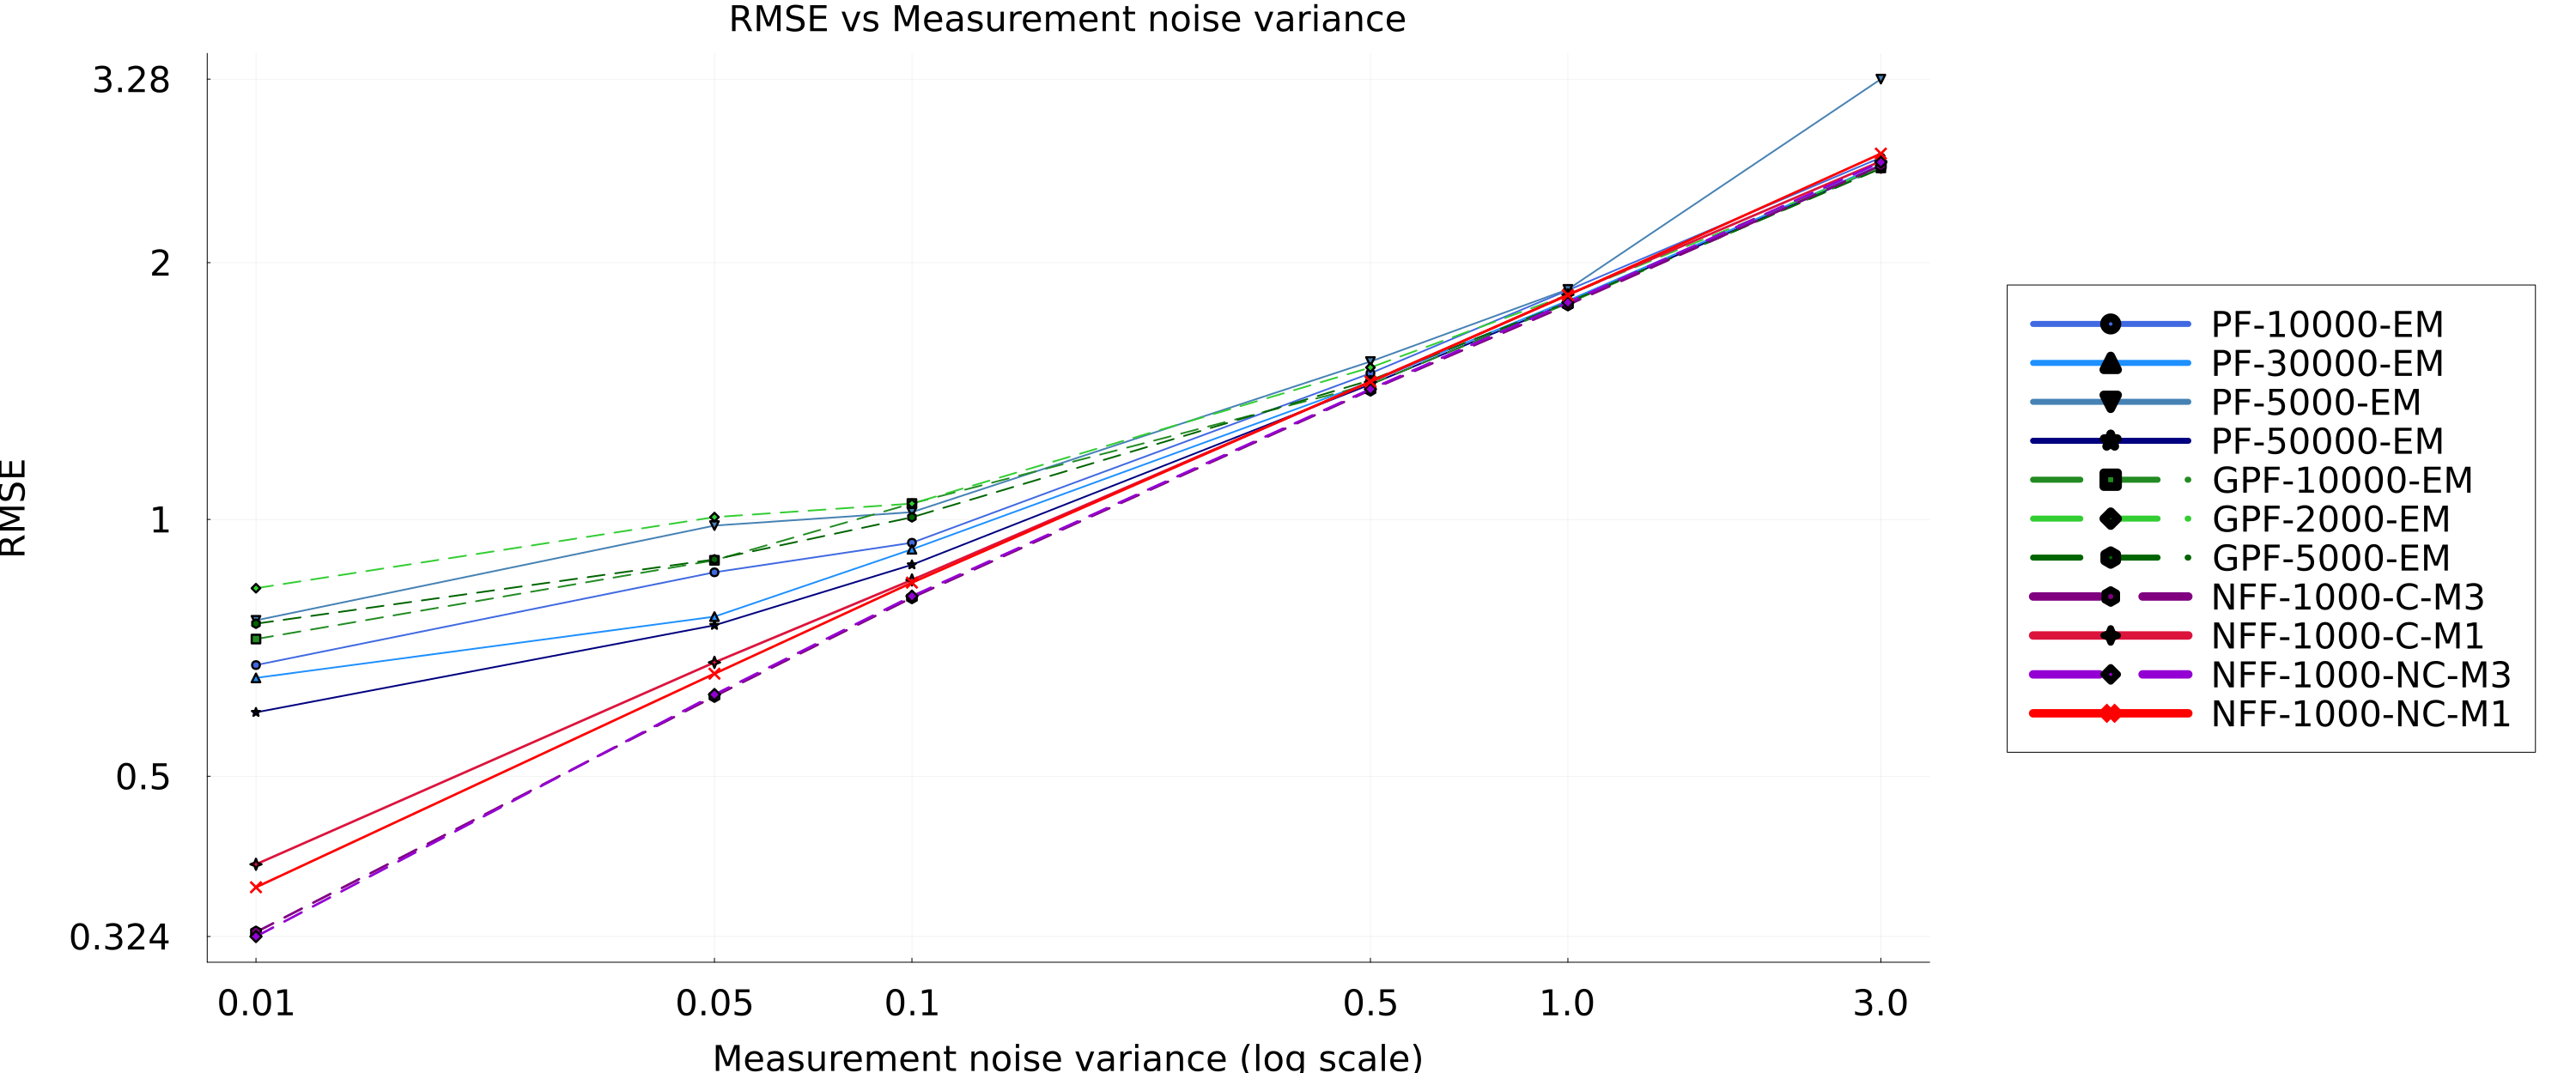
\includegraphics[width=\textwidth]{figures/Experiment06/rmse_nff_N1000_vs_others_rmse.png}
		\caption{RMSE vs. measurement noise variance.}
		\label{fig:noise_rmse}
	\end{SubFigure}
	
	\vspace{1.5em}
	
	\begin{SubFigure}{\textwidth}
		\centering
		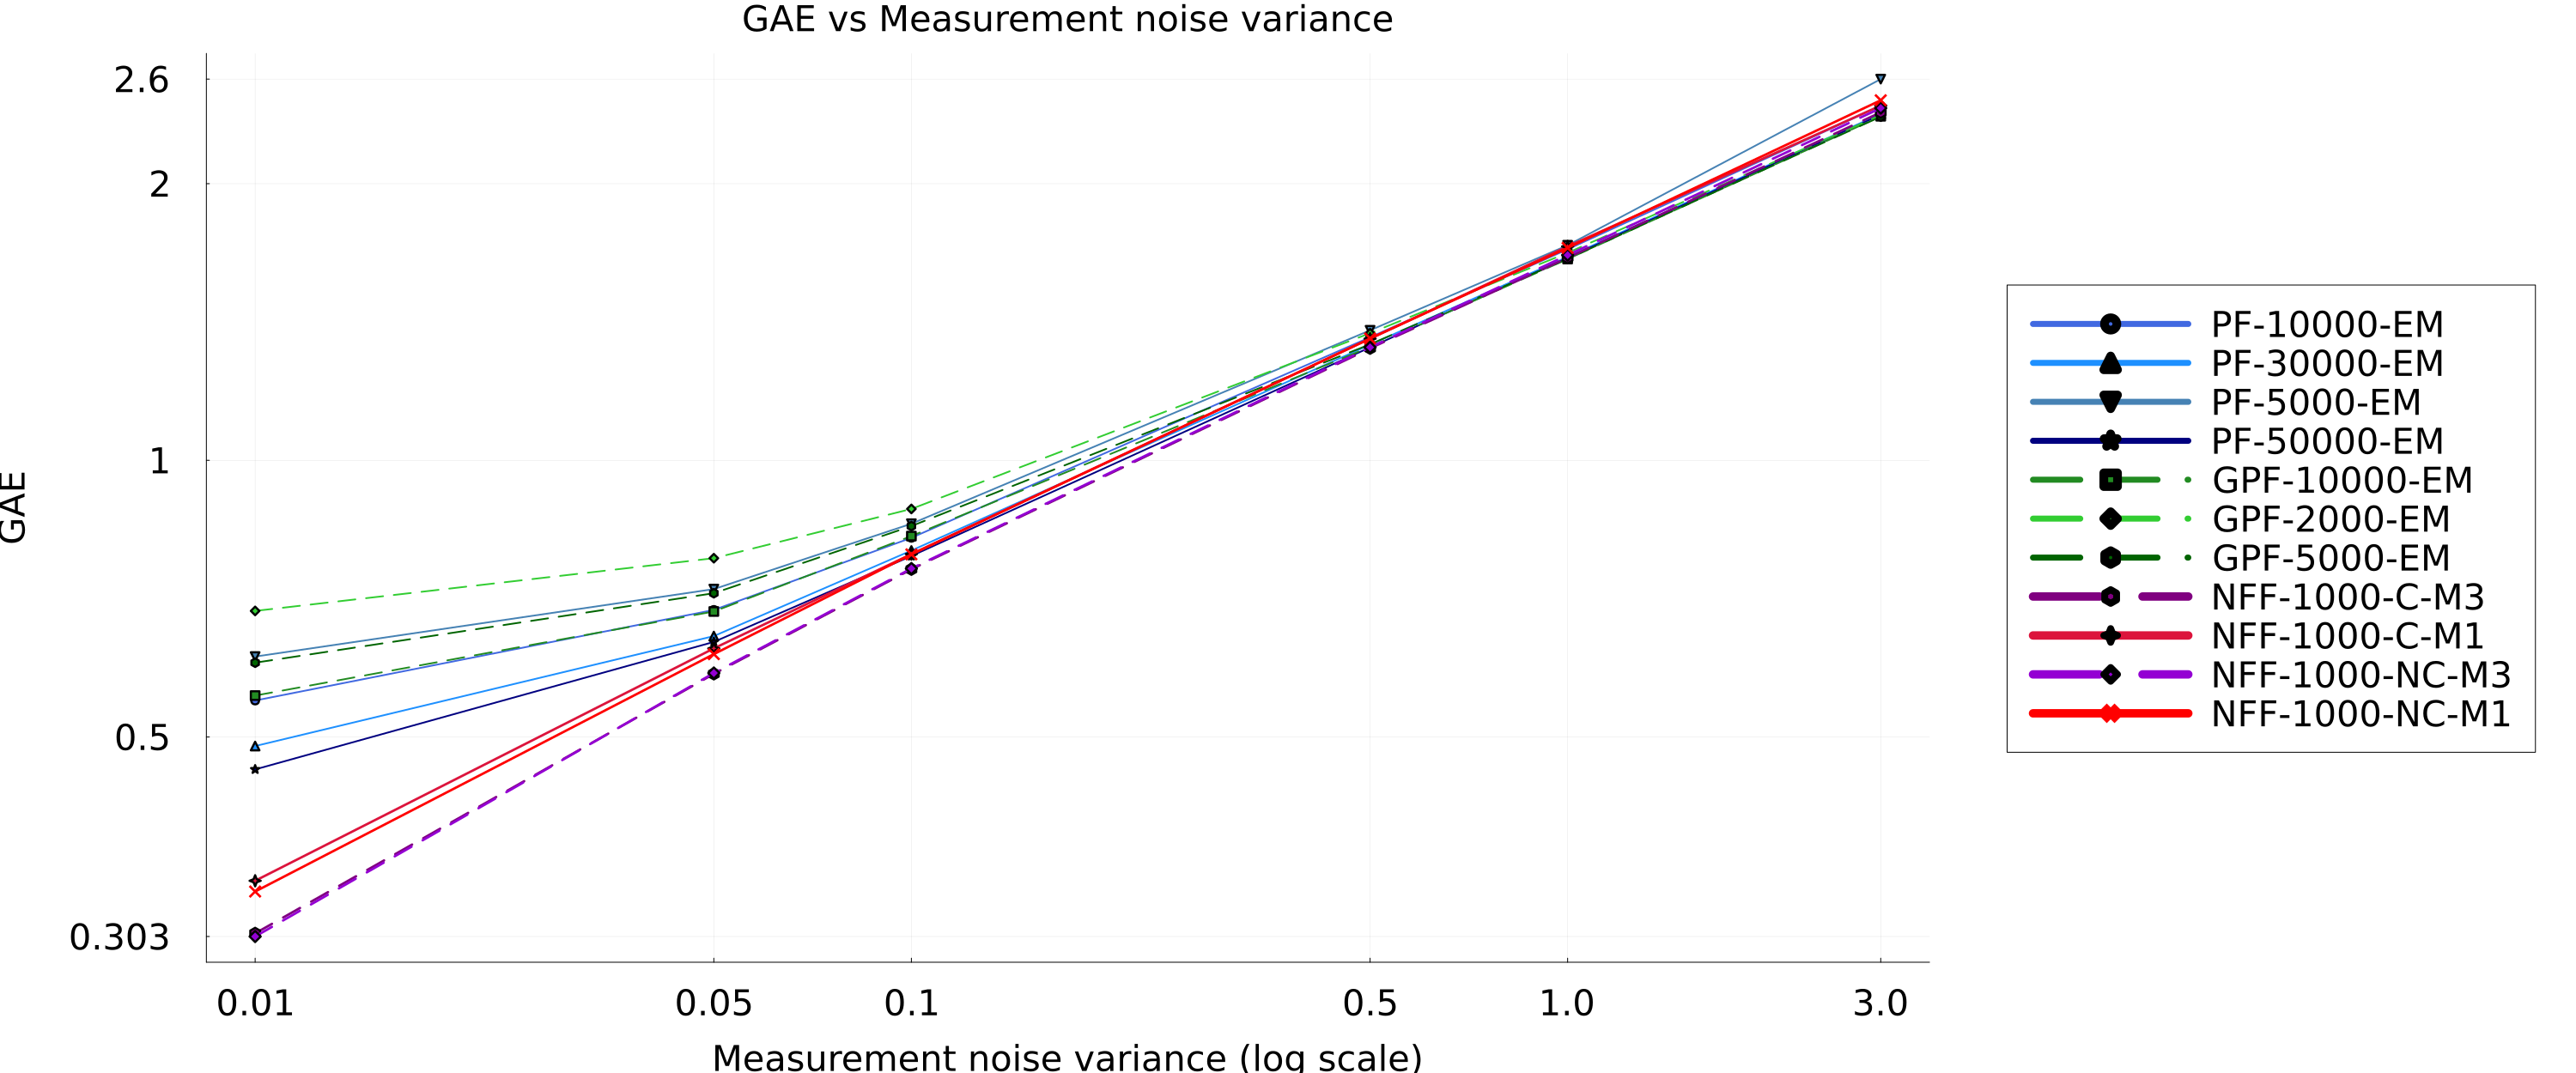
\includegraphics[width=\textwidth]{figures/Experiment06/gae_nff_N1000_vs_others_gae.png}
		\caption{GAE vs. measurement noise variance.}
		\label{fig:noise_gae}
	\end{SubFigure}
	\caption{RMSE and GAE vs. measurement noise variance.}
	\label{fig:noise_rmse_gae}
\end{Figure}

MERF reflects whether a filter effectively suppresses observation noise. Theoretically, in an ideal linear Gaussian setting with measurement noise variance 0.01 and prior cumulative system noise variance 0.1, the fused posterior noise variance is approximately $(0.1^{-1} + 0.01^{-1})^{-1} = 0.00909$. The corresponding ideal MERF value is $0.00909 / 0.01 = 0.909$. This indicates that when the sensor is already highly accurate, the theoretical room for further noise reduction by the filter is very limited.

In practical high-dimensional nonlinear systems, discretization error and particle approximation error make this ideal MERF almost unattainable. The experimental results in \Fig{fig:noise_merf} show that NFF with the third prediction mechanism maintains a MERF very close to 1.0. This means that it preserves the quality of the highly accurate observations without introducing substantial additional error. In contrast, PF with 50000 particles amplifies the original error by a factor of 1.87 after filtering, while GPF with 10000 particles amplifies it by more than a factor of 2. In the measurement-noise range from 0.05 to 0.1, the noise-suppression capability of NFF remains superior to that of PF and GPF. Only when the measurement noise increases further do the MERF values of all three filters converge.

\begin{Figure}[ht]
	\centering
	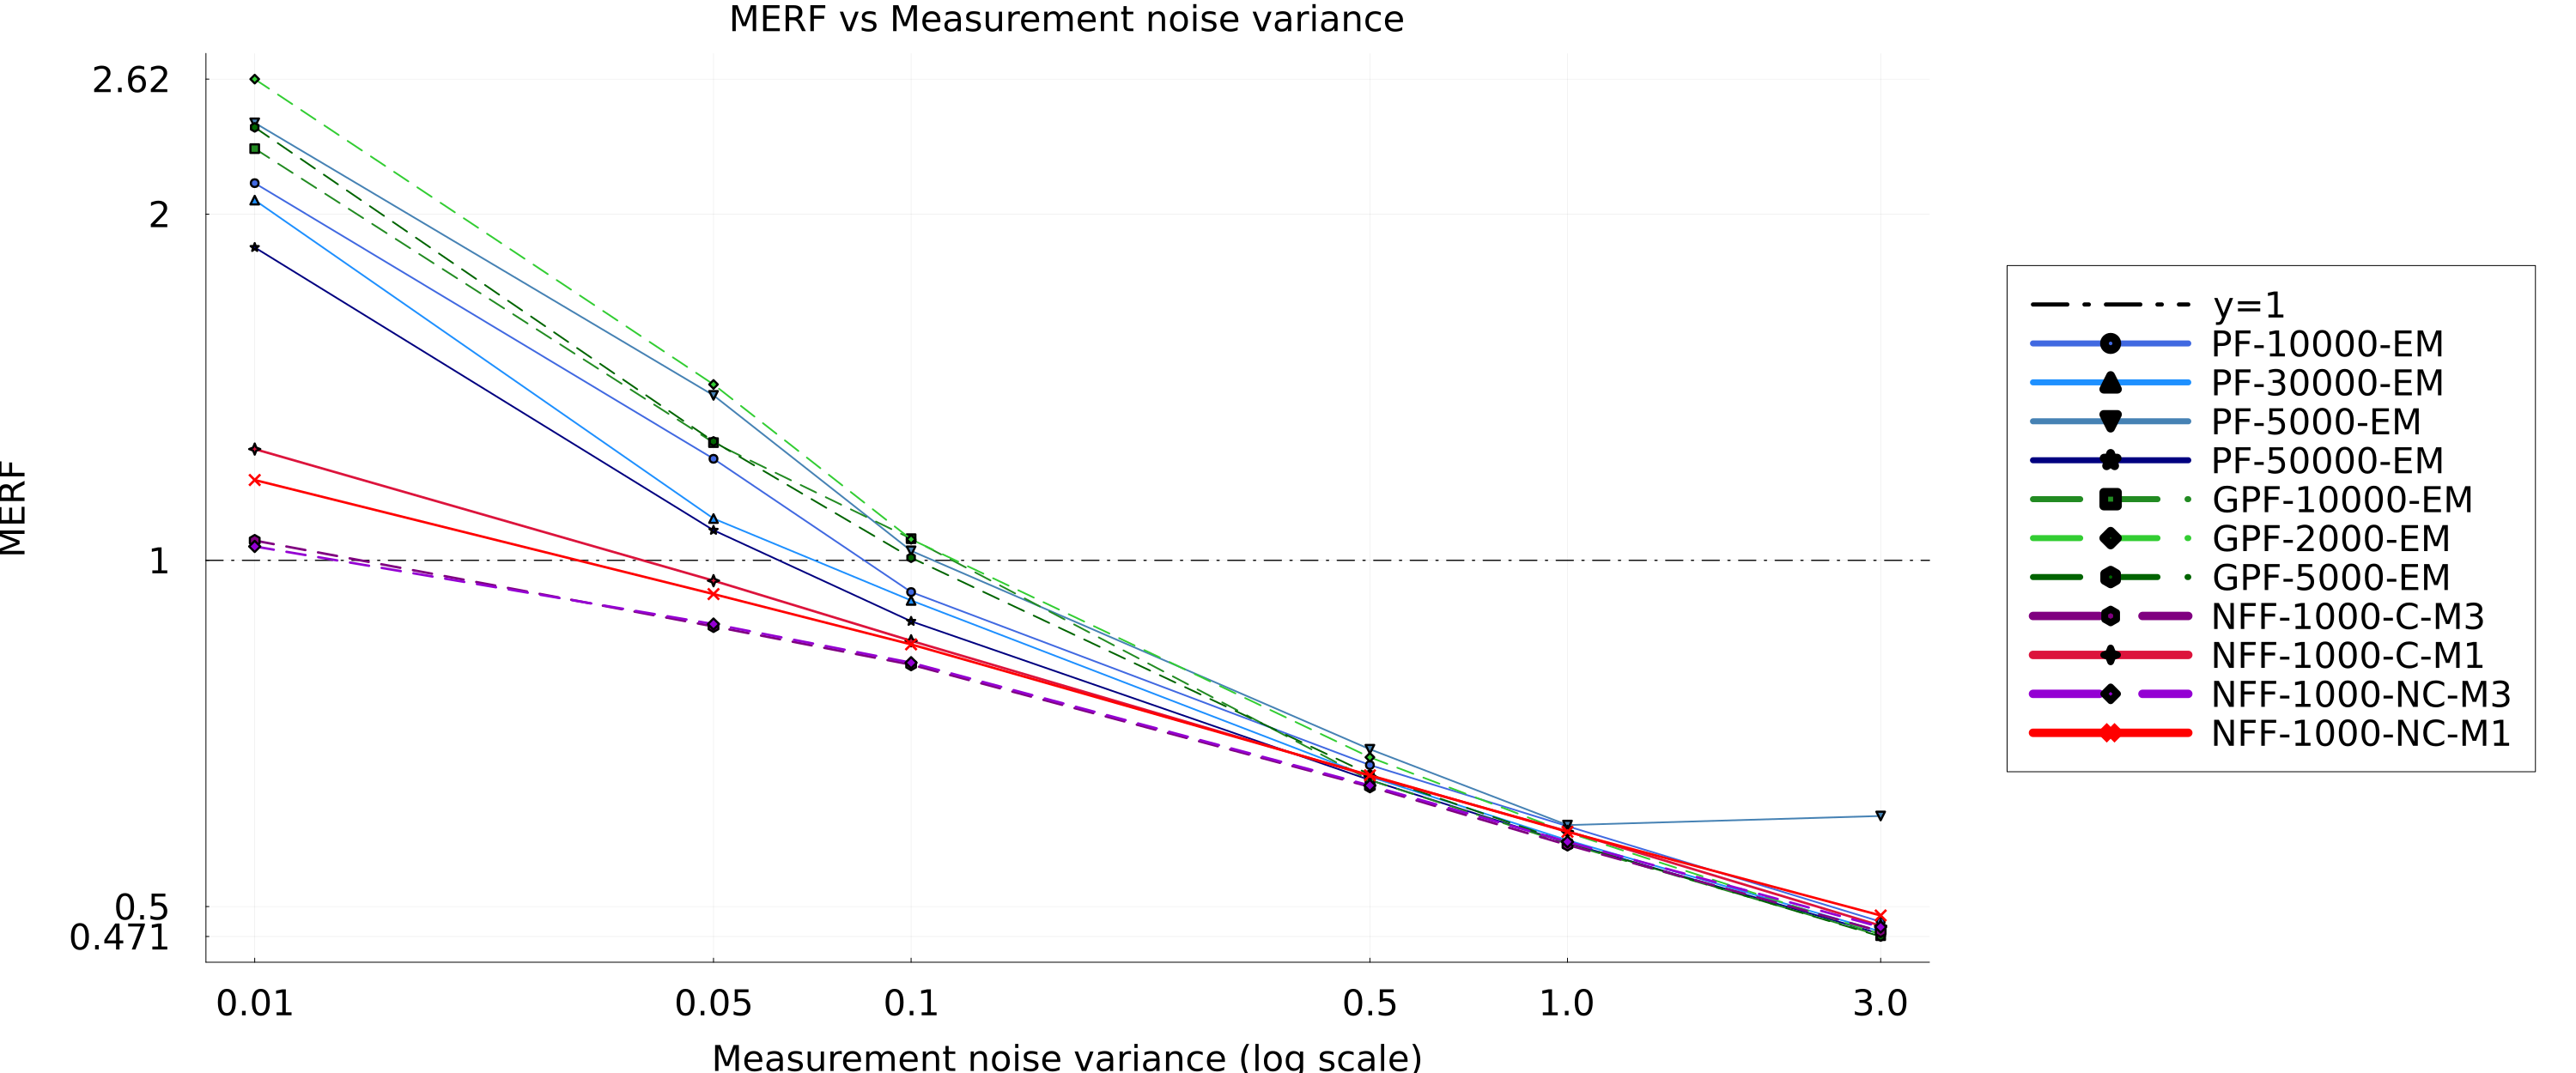
\includegraphics[width=\textwidth]{figures/Experiment06/merf_nff_N1000_vs_others_merf.png}
	\caption{MERF vs. measurement noise variance.}
	\label{fig:noise_merf}
\end{Figure}

ANEES is used to assess whether the filter becomes overconfident. As shown in \Fig{fig:noise_anees}, NFF with the third prediction mechanism behaves very stably, with ANEES consistently remaining below 2. This indicates that even under extremely narrow observation likelihoods, NFF maintains a sufficiently dispersed particle structure and that its estimated covariance reflects the actual estimation error reasonably well.

By contrast, for PF and GPF, when the measurement noise is extremely small (0.01 to 0.1), the narrow likelihood in the high-dimensional space causes severe particle degeneracy and sample impoverishment. The ANEES values of these two filters far exceed 100 and are therefore not visible in the plot because of the plotting scale. This implies that the particle sets of PF and GPF contract excessively and may even collapse to a single point, leading to severe overconfidence. Only when the measurement noise increases and the likelihood broadens do the ANEES values of PF and GPF return to normal levels and become comparable to those of NFF.

\begin{Figure}[ht]
	\centering
	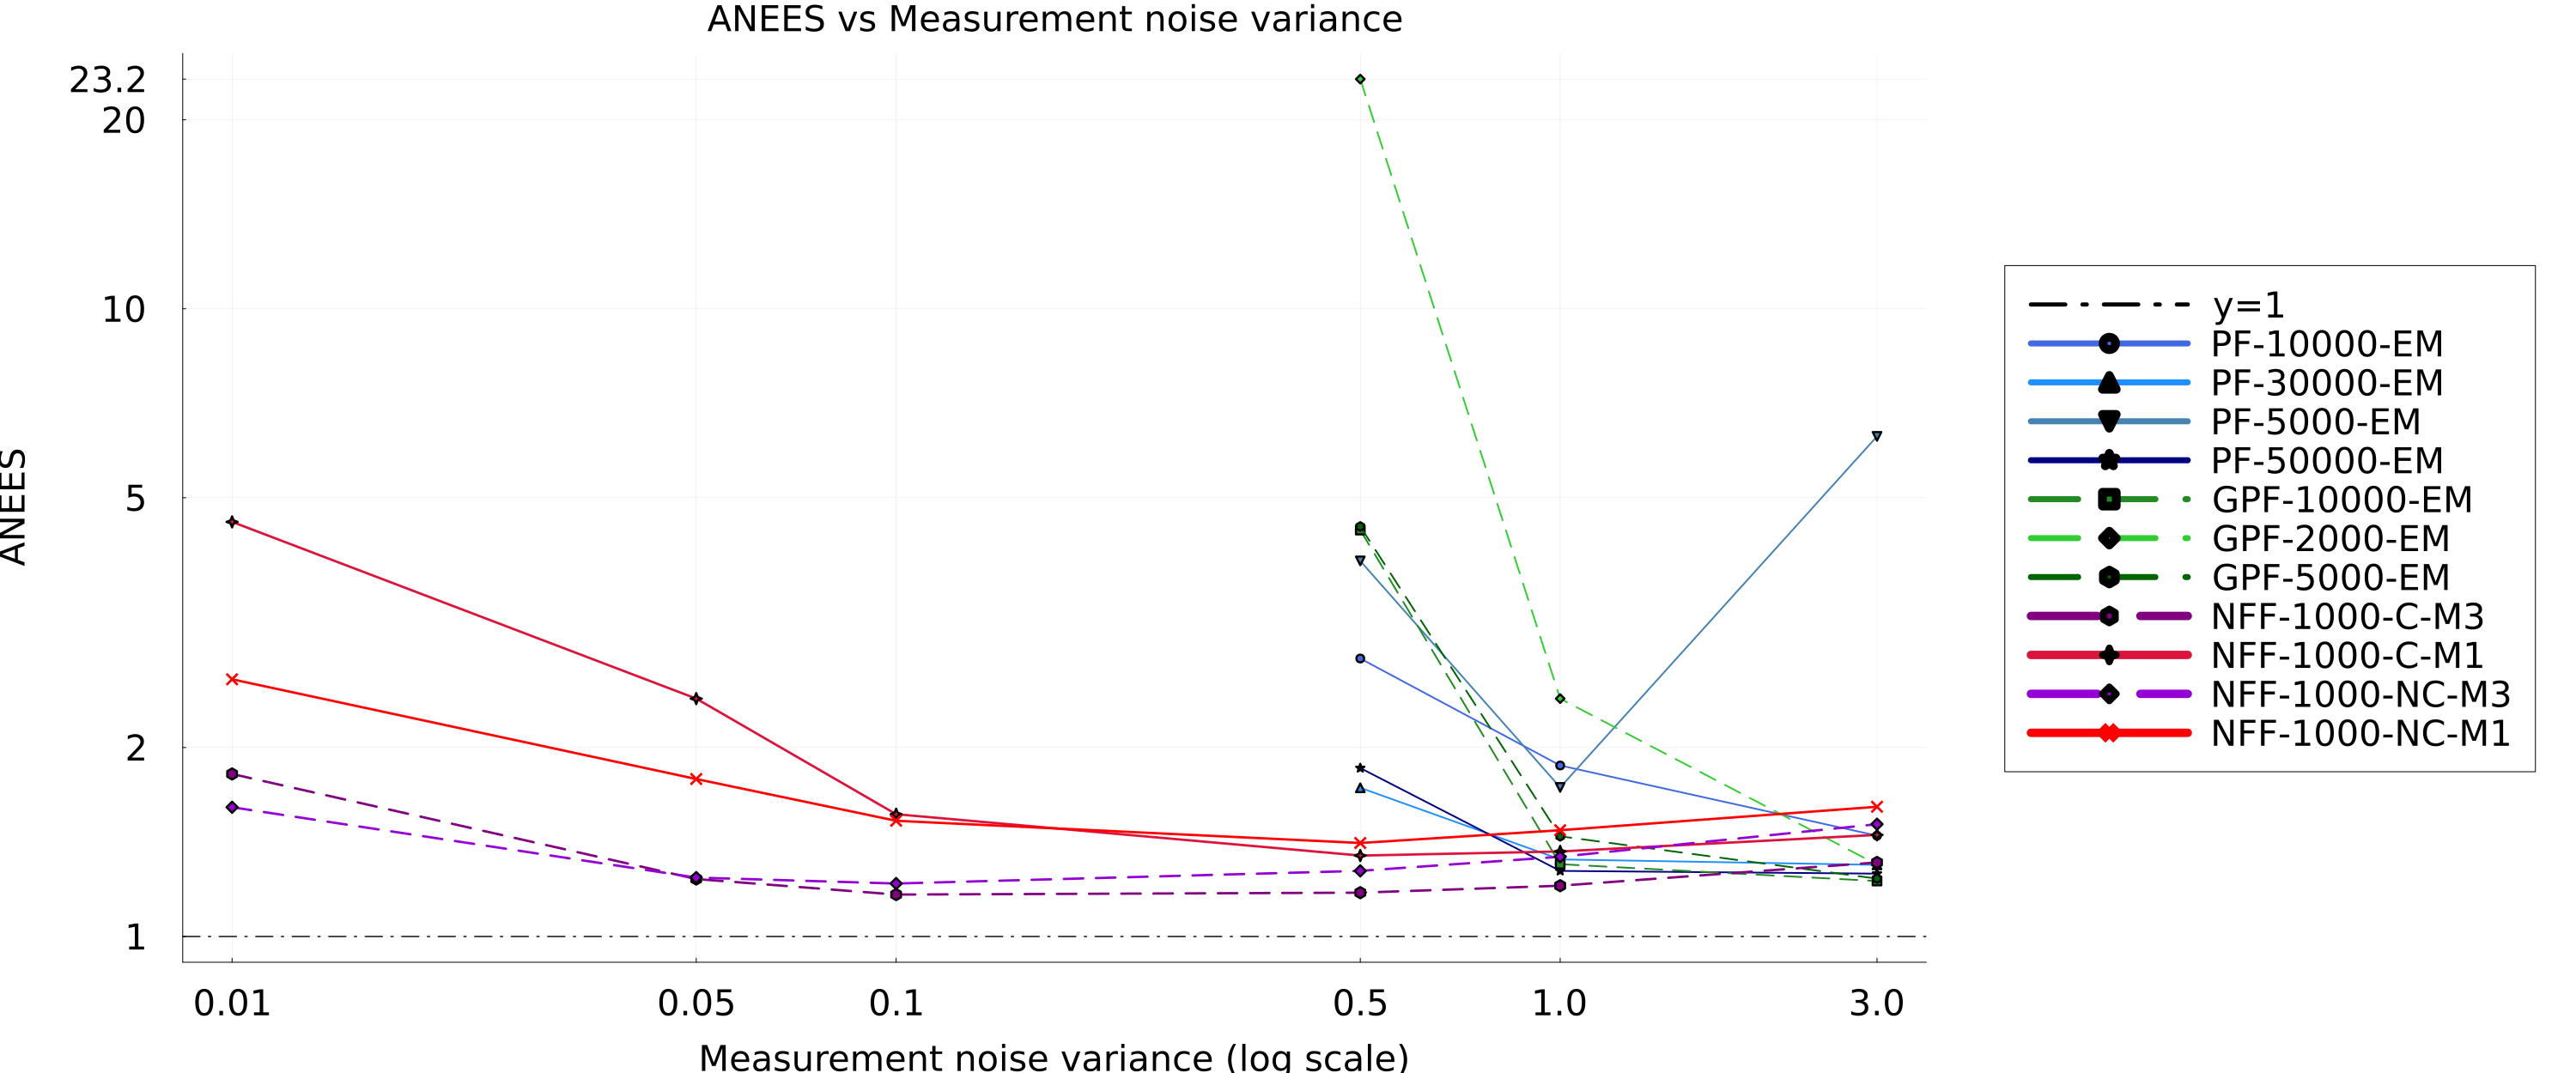
\includegraphics[width=\textwidth]{figures/Experiment06/anees_nff_N1000_vs_others_anees.png}
	\caption{ANEES vs. measurement noise variance.}
	\label{fig:noise_anees}
\end{Figure}

Taken together, these results show that in high-precision observation environments, traditional particle filters are highly susceptible to particle collapse and error amplification. In contrast, NFF effectively preserves particle diversity and exhibits a clear advantage in such scenarios.

\clearpage

\subsection{System Process Noise}
\label{subsec:system_noise}

This experiment evaluates the performance of different filters under different levels of system process noise. The measurement noise variance is fixed at 0.5. The control variable is the intensity of the system process noise, which is set to the sequence [0.1, 0.5, 1.0, 5.0, 10.0, 20.0]. After discretization, this corresponds to cumulative process noise variances per step of [0.01, 0.05, 0.1, 0.5, 1.0, 2.0].

In terms of state estimation accuracy, the RMSE and GAE curves in \Fig{fig:sysnoise_rmse_gae} show that the errors of all filters increase as the system process noise becomes larger. However, the accuracy curves of NFF gradually separate from those of PF and GPF. When the system noise is small (e.g., 0.1 and 0.5), the estimation accuracies of NFF, PF, and GPF are relatively similar. As the system noise continues to increase, the error growth of NFF remains noticeably slower, and the performance gap between NFF and the other two filters widens progressively.

\begin{Figure}[ht]
	\centering
	\begin{SubFigure}{\textwidth}
		\centering
		
\includegraphics[width=\textwidth]{figures/Experiment07/rmse_nff_N1000_vs_others_rmse.png}
		\caption{RMSE vs. system noise variance.}
		\label{fig:sysnoise_rmse}
	\end{SubFigure}
	
	\vspace{1.5em}
	
	\begin{SubFigure}{\textwidth}
		\centering
		
\includegraphics[width=\textwidth]{figures/Experiment07/gae_nff_N1000_vs_others_gae.png}
		\caption{GAE vs. system noise variance.}
		\label{fig:sysnoise_gae}
	\end{SubFigure}
	\caption{RMSE and GAE vs. system noise variance.}
	\label{fig:sysnoise_rmse_gae}
\end{Figure}

The MERF results further emphasize the advantage of NFF. The data in \Fig{fig:sysnoise_merf} shows that the larger the system noise becomes, the better NFF performs relative to PF and GPF in suppressing observation noise. Under extreme high-interference conditions, where the system process noise intensity reaches 20.0, the MERF of NFF remains below 1.0 (approximately 0.8), meaning that effective noise reduction is still achieved. In contrast, under the same conditions, the MERF values of PF and GPF are far above 1.0, indicating that their filtering updates actually amplify the original measurement error substantially.

\begin{Figure}[ht]
	\centering
	
\includegraphics[width=\textwidth]{figures/Experiment07/merf_nff_N1000_vs_others_merf.png}
	\caption{MERF vs. system noise variance.}
	\label{fig:sysnoise_merf}
\end{Figure}

In terms of ANEES, NFF shows excellent robustness. As illustrated in \Fig{fig:sysnoise_anees}, its ANEES remains below 2 across all tested system noise levels and stays very close to 1 when the system noise is extremely large. This indicates that NFF maintains a realistic assessment of its estimation uncertainty while preserving a reasonable particle structure. By contrast, PF and GPF can maintain a somewhat dispersed particle structure only when the system noise is small. As the system noise increases, the ANEES values of PF and GPF rise rapidly and exceed 100, again truncated in the plot because of the scale. This indicates that under high system noise, the particle sets of PF and GPF undergo severe over-contraction and may collapse to a single point, causing the covariance estimate to fail completely and the filters to become extremely overconfident.

\begin{Figure}[ht]
	\centering
	
\includegraphics[width=\textwidth]{figures/Experiment07/anees_nff_N1000_vs_others_anees.png}
	\caption{ANEES vs. system noise variance.}
	\label{fig:sysnoise_anees}
\end{Figure}

Overall, these results indicate that NFF is better suited to high-dimensional complex systems with large process noise and is more capable of extracting useful information from highly noisy environments to reduce observation error.

The underlying reason is the difference in how the prior information is utilized. When the system process noise is very large, the prior particle set generated by the prediction step becomes highly dispersed and sparse in the state space. For PF and GPF, only a very small number of particles fall within the effective support of the likelihood, while the vast majority are effectively discarded after the weight update. As a result, most of the prior information generated by the system dynamics is wasted. By contrast, NFF uses a homotopy mechanism to drive the dispersed prior particles smoothly toward the posterior region, thereby making much more effective use of the prior information.
\clearpage

\section{Sensitivity to System Nonlinearity Intensity}
\label{sec:nonlinearity_sensitivity}

This experiment evaluates the filtering performance under different levels of system nonlinearity. The system process noise is fixed at 1, and the measurement noise variance is fixed at 0.5. The control variable is the discretization time step $\Delta t$, which is set to the sequence [0.01, 0.1, 0.15, 0.4, 0.6]. In a nonlinear system, a larger integration step $\Delta t$ implies stronger nonlinearity within a single propagation step, making the system evolution increasingly difficult to predict.

In terms of state estimation accuracy, the RMSE and GAE curves in \Fig{fig:nonlinear_rmse_gae} show that the errors of all filters increase as the discretization step $\Delta t$ becomes larger and the state evolution becomes harder to predict. When $\Delta t$ is small (0.01 to 0.15), the accuracy of NFF is comparable to that of PF and GPF. However, as the step size increases further to 0.4 and 0.6, the accuracy curves of NFF begin to separate from those of PF and GPF. The error growth of NFF is noticeably smaller, indicating better estimation capability under strongly nonlinear conditions.

\begin{Figure}[ht]
	\centering
	\begin{SubFigure}{\textwidth}
		\centering
		
\includegraphics[width=\textwidth]{figures/Experiment08/rmse_nff_N1000_vs_others_rmse.png}
		\caption{RMSE vs. discretization time step.}
		\label{fig:nonlinear_rmse}
	\end{SubFigure}
	
	\vspace{1.5em}
	
	\begin{SubFigure}{\textwidth}
		\centering
		
\includegraphics[width=\textwidth]{figures/Experiment08/gae_nff_N1000_vs_others_gae.png}
		\caption{GAE vs. discretization time step.}
		\label{fig:nonlinear_gae}
	\end{SubFigure}
	\caption{RMSE and GAE vs. discretization time step.}
	\label{fig:nonlinear_rmse_gae}
\end{Figure}

MERF clearly reflects the noise-rejection performance of the filters under strong model nonlinearity. As shown in \Fig{fig:nonlinear_merf}, when $\Delta t$ lies between 0.01 and 0.15, the performance gap among the filters is relatively small. A clear turning point appears at $\Delta t = 0.4$. At this point, the system nonlinearity is already very strong, and the update steps of PF and GPF actually amplify the measurement noise, with MERF far above 1. By contrast, NFF still reduces the observation noise effectively.

However, when the step size is increased further to the extreme value $\Delta t = 0.6$, the large time interval makes the prediction step highly inaccurate. At this stage, the prediction step provides little useful prior information for the update and may even provide misleading information. Under this extreme condition, where the prediction model itself essentially fails, the MERF values of NFF, PF, and GPF all deteriorate severely.

\begin{Figure}[ht]
	\centering
	
\includegraphics[width=\textwidth]{figures/Experiment08/merf_nff_N1000_vs_others_merf.png}
	\caption{MERF vs. discretization time step.}
	\label{fig:nonlinear_merf}
\end{Figure}

The ANEES results in \Fig{fig:nonlinear_anees} further support this interpretation. When $\Delta t$ is small (0.01 to 0.1), PF, GPF, and NFF all maintain a reasonable particle structure and do not show obvious overconfidence. However, when $\Delta t$ increases to 0.4 and 0.6, the ANEES values of PF and GPF exceed 100, indicating that under strong nonlinear mappings their particle sets again suffer severe degeneracy and collapse.

It is worth noting that NFF also exhibits overconfidence when $\Delta t$ is large, as reflected by its significantly increased ANEES value. This is not caused by particle collapse in NFF, but rather by the fact that the overly large time interval makes the predicted prior positions highly inaccurate. This large prediction bias then affects the final update result, producing a larger actual estimation error.

\begin{Figure}[ht]
	\centering
	
\includegraphics[width=\textwidth]{figures/Experiment08/anees_nff_N1000_vs_others_anees.png}
	\caption{ANEES vs. discretization time step.}
	\label{fig:nonlinear_anees}
\end{Figure}

Taken together, these results suggest that NFF is well suited to strongly nonlinear scenarios in which prediction is difficult. As long as the state evolution equation can still provide at least a small amount of useful prior information, NFF is much more capable than PF and GPF of exploiting this weak information to suppress observation noise. However, if the nonlinearity becomes so strong that the prediction model fails completely and no longer provides valid prior information, NFF also suffers unavoidable performance degradation.

\clearpage

\section{Sensitivity to Model Mismatch}
\label{sec:mismatch_sensitivity}

To evaluate the performance of each filter under non-ideal conditions, this experiment introduces model mismatch artificially. Perturbations of $\pm 20\%$ are applied to the system process noise covariance matrix $Q$, the measurement noise covariance matrix $R$, the state model $f(x)$, and the observation model $h(x)$ in order to assess the robustness of the algorithms.

When perturbations are applied to the noise parameters (overestimated or underestimated $Q$ and $R$) and the observation model (overestimated or underestimated $h(x)$), the results show that NFF with 1000 particles performs comparably to the best PF configuration with up to 50000 particles and the best GPF configuration with 10000 particles. As reported in \Tab{tab:full_mismatch_results_v2}, the differences in three of the four error metrics (RMSE, GAE, and MERF) remain comparable, whereas NFF outperforms PF and GPF in ANEES. This indicates that while all three filters maintain basic robustness to moderate mismatches, NFF estimates its own uncertainty more accurately.

However, when a $+20\%$ mismatch is introduced into the system model $f(x)$, NFF exhibits a clear advantage in estimation accuracy. Compared with the best PF and GPF results, its RMSE is reduced by about $18\%$--$29\%$, while its MERF is improved by approximately $17\%$--$28\%$. More importantly, in terms of ANEES, which reflects filter consistency, both PF and GPF collapse completely under this condition, with ANEES diverging to \textit{NaN}. In contrast, both variants of NFF (M1 and M3) remain stable and convergent, with ANEES staying within a clearly reasonable range.

The fundamental reason why NFF remains highly robust to mismatch in the system model is consistent with the mechanism discussed earlier. Even when the prediction is no longer sufficiently accurate, NFF can still exploit the prior information effectively.

\begin{Table}[ht]
	\caption{Performance under $\pm 20\%$ model mismatches. Comparison between the best PF/GPF and NFF ($L=1000$).}
	\label{tab:full_mismatch_results_v2}
	\footnotesize
	\setlength{\tabcolsep}{5pt}
	\begin{tabular}{|c|l|c|c|cc|cc|}
		\hline
		& & & & \multicolumn{2}{c|}{NFF (C)} & \multicolumn{2}{c|}{NFF (NC)} \\ \cline{5-8}
		Mismatch Type & Metric & Best PF & Best GPF & M3  & M1  & M3  & M1  \\ \hline
		
		{$+20\% Q$}
		& RMSE  & 1.459 & 1.469 & \textbf{1.409} & 1.439 & 1.410 & 1.444 \\
		& GAE   & 1.344 & 1.348 & \textbf{1.318} & 1.346 & 1.319 & 1.350 \\
		& MERF  & 0.653 & 0.657 & \textbf{0.631} & 0.645 & 0.632 & 0.647 \\
		& ANEES & 1.398 & 1.935 & \textbf{1.071} & 1.209 & 1.141 & 1.274 \\ \hline
		
		{$-20\% Q$}
		& RMSE  & 1.519 & 1.875 & \textbf{1.432} & 1.483 & 1.445 & 1.495 \\
		& GAE   & 1.385 & 1.397 & \textbf{1.338} & 1.386 & 1.346 & 1.396 \\
		& MERF  & 0.679 & 0.839 & \textbf{0.645} & 0.668 & 0.648 & 0.670 \\
		& ANEES & 1.785 & NaN   & \textbf{1.344} & 1.585 & 1.480 & 1.686 \\ \hline
		
		{$+20\% R$}
		& RMSE  & 1.484 & 1.484 & \textbf{1.459} & 1.479 & 1.464 & 1.499 \\
		& GAE   & \textbf{1.362} & \textbf{1.362} & 1.406 & 1.426 & 1.411 & 1.443 \\
		& MERF  & \textbf{0.664} & \textbf{0.664} & \textbf{0.664} & 0.673 & 0.666 & 0.682 \\
		& ANEES & 1.265 & 1.629 & \textbf{1.133} & 1.239 & 1.237 & 1.430 \\ \hline
		
		{$-20\% R$}
		& RMSE  & 1.479 & 1.490 & \textbf{1.432} & 1.451 & 1.435 & 1.461 \\
		& GAE   & \textbf{1.356} & 1.362 & 1.379 & 1.398 & 1.382 & 1.410 \\
		& MERF  & 0.662 & 0.667 & \textbf{0.652} & 0.660 & 0.653 & 0.665 \\
		& ANEES & 1.878 & 7.101 & \textbf{1.344} & 1.478 & 1.443 & 1.620 \\ \hline
		
		{$+20\% f(x)$}
		& RMSE  & 1.947 & 2.227 & \textbf{1.581} & 1.645 & 1.606 & 1.666 \\
		& GAE   & 1.550 & 1.575 & \textbf{1.534} & 1.602 & 1.559 & 1.616 \\
		& MERF  & 0.871 & 0.996 & \textbf{0.720} & 0.749 & 0.731 & 0.758 \\
		& ANEES & NaN   & NaN   & \textbf{1.508} & 1.846 & 1.720 & 2.050 \\ \hline
		
		{$-20\% f(x)$}
		& RMSE  & 1.666 & 1.668 & \textbf{1.578} & 1.657 & 1.607 & 1.681 \\
		& GAE   & 1.554 & 1.548 & \textbf{1.524} & 1.599 & 1.554 & 1.631 \\
		& MERF  & 0.745 & 0.746 & \textbf{0.718} & 0.754 & 0.731 & 0.765 \\
		& ANEES & 2.005 & 2.801 & \textbf{1.418} & 1.785 & 1.607 & 1.987 \\ \hline
		
		{$+20\% h(x)$}
		& RMSE  & 2.649 & 2.663 & 2.509 & 2.585 & \textbf{2.497} & 2.514 \\
		& GAE   & 2.528 & 2.534 & 2.452 & 2.528 & \textbf{2.440} & 2.453 \\
		& MERF  & 0.852 & 0.856 & 0.833 & 0.858 & \textbf{0.829} & 0.834 \\
		& ANEES & 9.071 & 24.620& \textbf{4.242} & 5.546 & 4.360 & 5.034 \\ \hline
		
		{$-20\% h(x)$}
		& RMSE  & 2.867 & 3.225 & 2.852 & 2.922 & \textbf{2.779} & 2.823 \\
		& GAE   & \textbf{2.681} & 2.777 & 2.799 & 2.874 & 2.731 & 2.775 \\
		& MERF  & 0.613 & 0.690 & 0.620 & 0.635 & \textbf{0.604} & 0.614 \\
		& ANEES & 14.986 & NaN  & \textbf{3.438} & 4.325 & 3.767 & 4.199 \\ \hline
	\end{tabular}
\end{Table}

\clearpage

\section{Extreme Condition Tests}
\label{sec:extreme_conditions}

This experiment considers four extreme combinations of system process noise $Q$ and observation noise $R$. Through these comparative tests, the advantages and applicable scenarios of NFF are clarified.

When the system is subject to both large system noise and large observation noise, prediction becomes difficult and the sensor measurements become highly unreliable. Under this severely adverse condition, all filters perform poorly, with errors increasing to very large values (all RMSE values approach 6.0). As shown in \Tab{tab:extreme_noise_v2}, the performance of NFF is not significantly different from that of PF and GPF.

When the system has small process noise but large observation noise, the likelihood function becomes broad and relatively flat in the state space. Under this condition, GPF achieves the best performance. NFF ranks second, but remains inferior to GPF.

In the scenario with small system noise and small observation noise, both the prior and the likelihood are highly concentrated. As a result, PF and GPF suffer from severe particle degeneracy, and their consistency metric (ANEES) collapses. NFF, by contrast, remains stable and reduces the RMSE by more than 20\% relative to PF and GPF.

In the scenario with large system noise and small observation noise, the results show that PF and GPF diverge completely. Not only do their ANEES values become NaN, but their filtering outputs also amplify the original measurement error by a factor of four to five, with MERF reaching 4.272 and 5.283, respectively. By contrast, NFF remains stable, improves the estimation accuracy by up to 70\%, and keeps MERF within a reasonable range.

A summary of the dominant performance regions for the different filters under these varied noise conditions is illustrated in \Fig{fig:noise_quadrant}.

\begin{Figure}[ht]
    \centering
    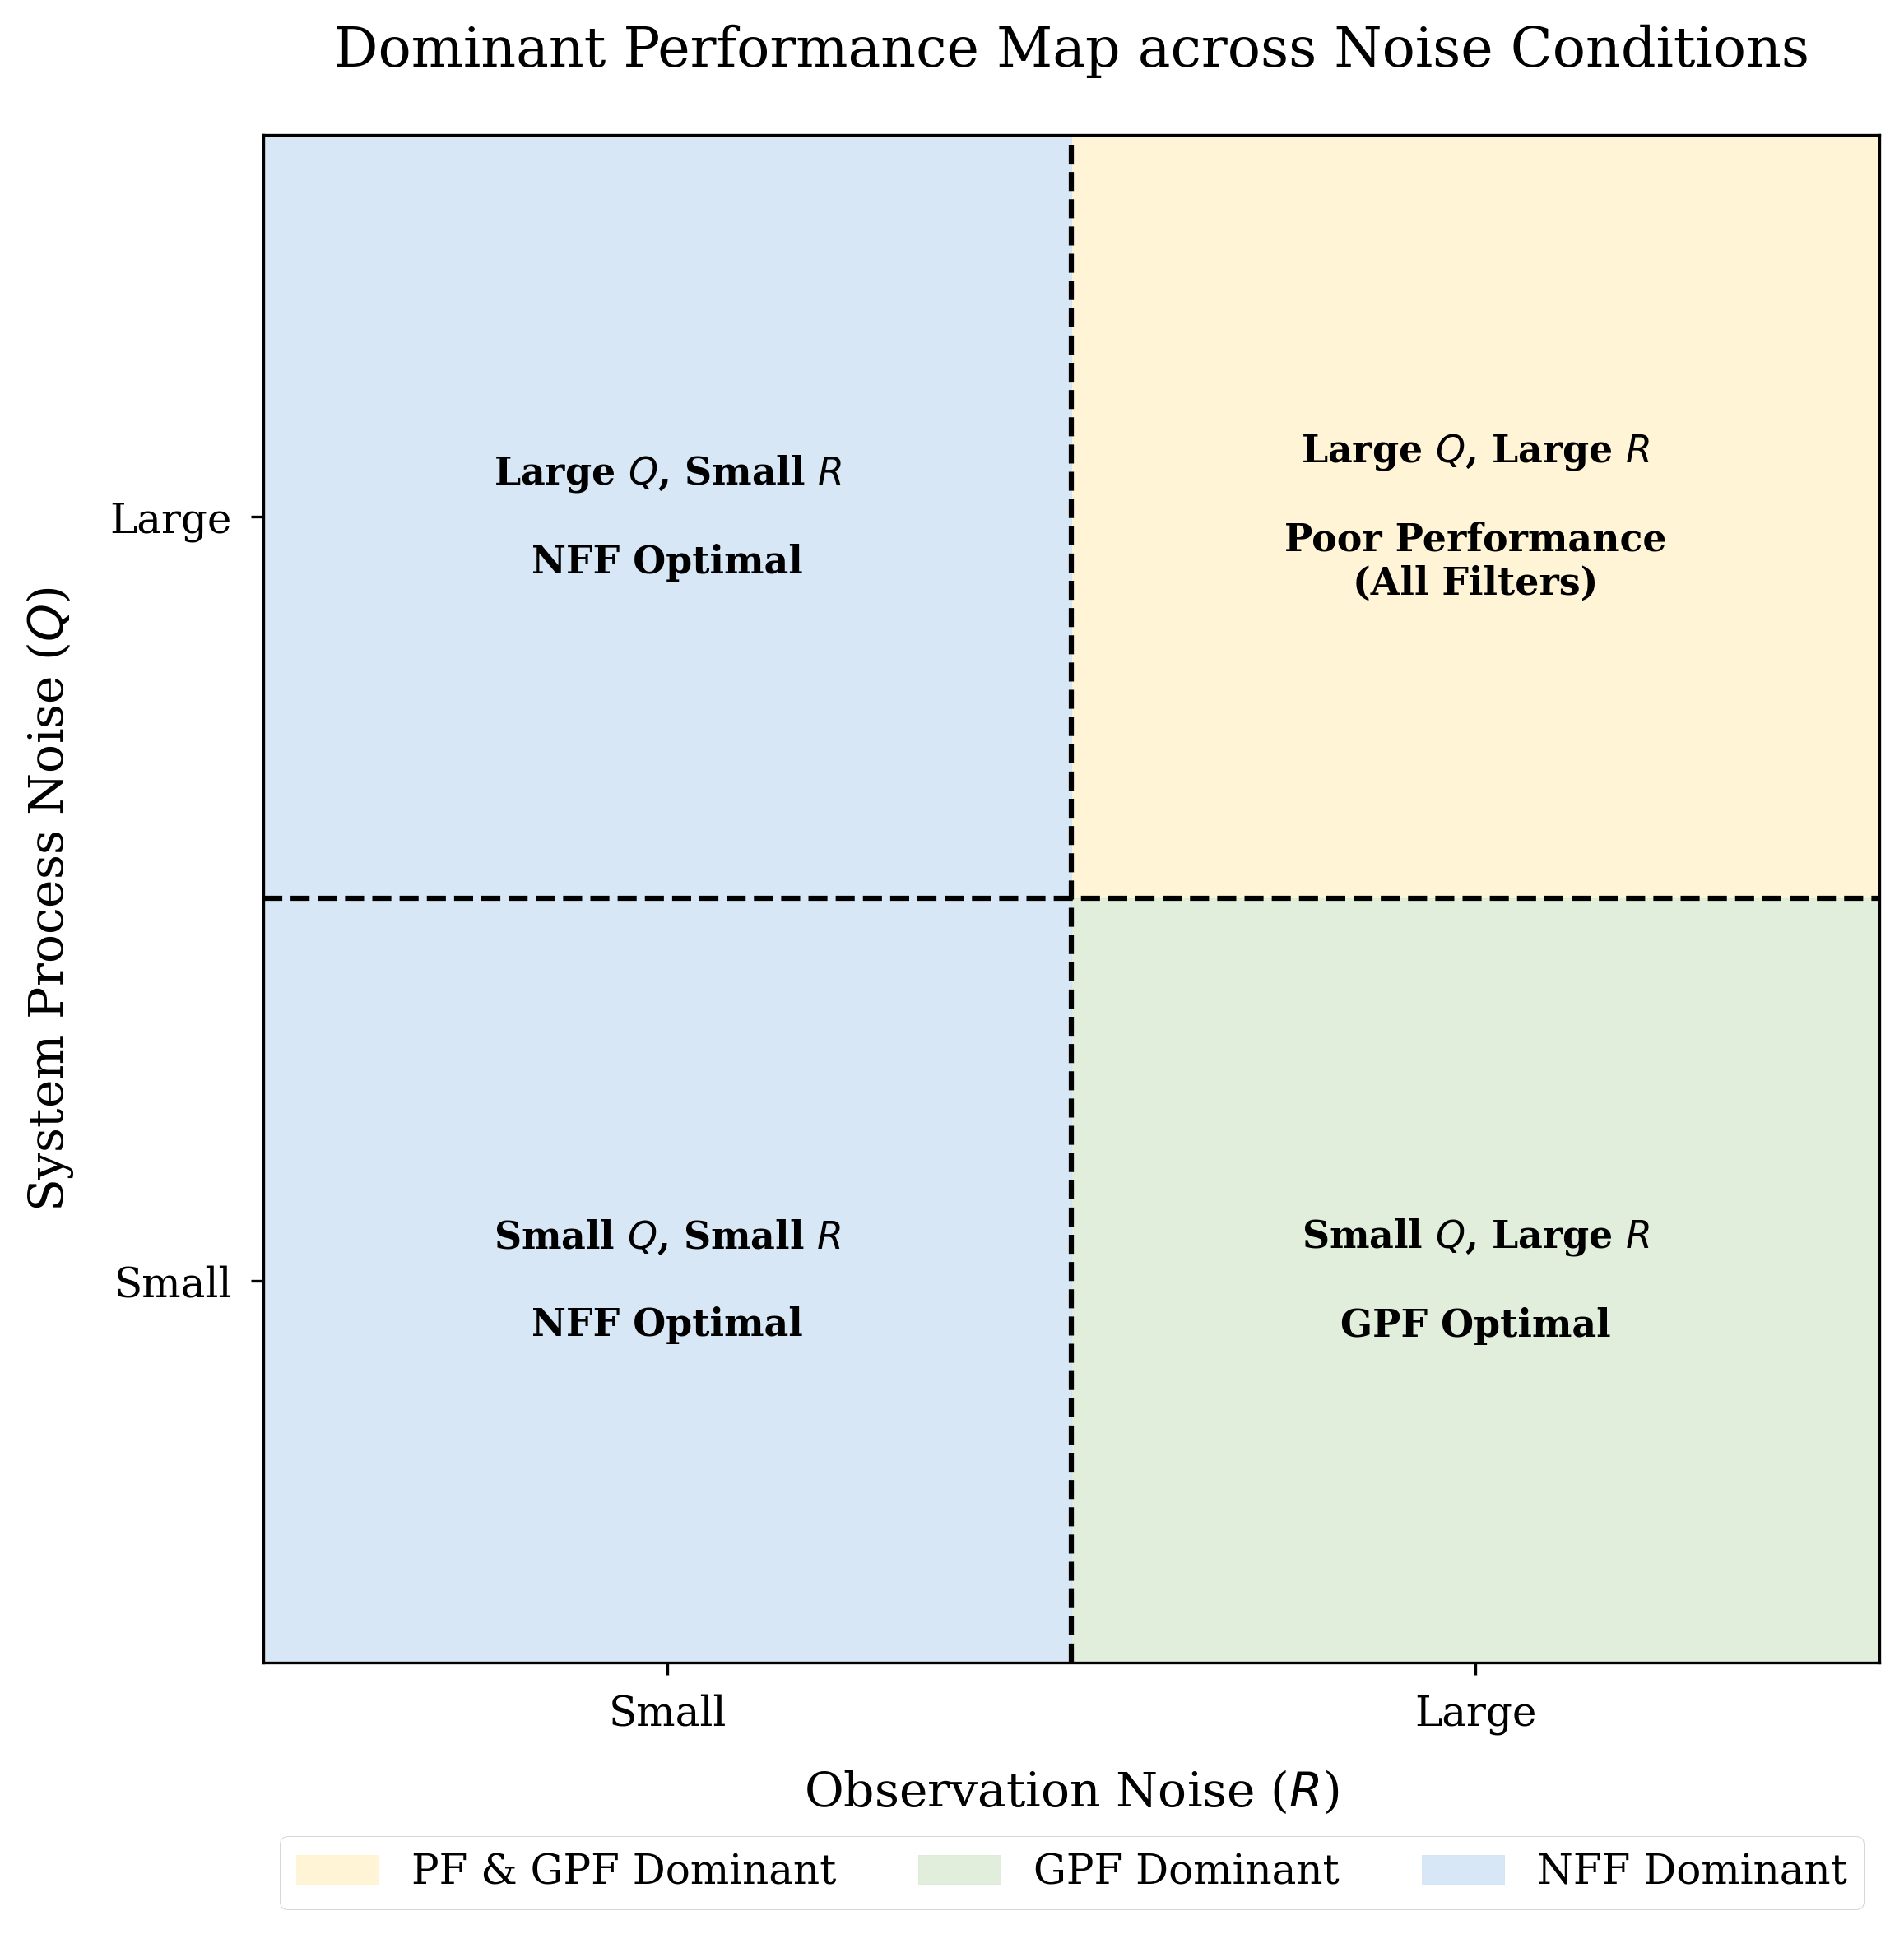
\includegraphics[width=0.9\textwidth]{figures/noise_quadrant.png}
    \caption{Dominant performance map of filters across different combinations of system process noise $Q$ and observation noise $R$.}
    \label{fig:noise_quadrant}
\end{Figure}

\begin{Table}[ht]
	\caption{Performance under extreme combinations of $Q$ and $R$. Comparison between best PF/GPF and NFF ($L=1000$).}
	\label{tab:extreme_noise_v2}
	\footnotesize
	\setlength{\tabcolsep}{5pt}
	\begin{tabular}{|c|l|c|c|cc|cc|}
		\hline
		& & & & \multicolumn{2}{c|}{NFF (C)} & \multicolumn{2}{c|}{NFF (NC)} \\ \cline{5-8}
		Condition & Metric & Best PF & Best GPF & M3 & M1 & M3 & M1 \\ \hline
		
		{Large $Q$ \& Large $R$} 
		& RMSE  & 5.668 & \textbf{5.644} & 5.662 & 5.793 & 5.793 & 5.875 \\
		& GAE   & 5.221 & \textbf{5.209} & 5.241 & 5.354 & 5.325 & 5.382 \\
		& MERF  & 0.567 & \textbf{0.565} & 0.567 & 0.581 & 0.581 & 0.589 \\
		& ANEES & \textbf{1.228} & 1.238 & 1.322 & 1.471 & 1.517 & 1.596 \\ \hline
		
		{Small $Q$ \& Large $R$} 
		& RMSE  & 12.007 & \textbf{3.715} & 5.036 & 5.043 & 7.097 & 6.926 \\
		& GAE   & 9.501  & \textbf{3.114} & 4.136 & 4.029 & 5.366 & 5.228 \\
		& MERF  & 1.201  & \textbf{0.372} & 0.505 & 0.505 & 0.711 & 0.694 \\
		& ANEES & NaN    & \textbf{3.306} & 41.513 & 43.444 & 51.552 & 82.882 \\ \hline
		
		{Small $Q$ \& Small $R$} 
		& RMSE  & 0.513 & 0.482 & \textbf{0.305} & 0.322 & 0.336 & 0.336 \\
		& GAE   & 0.469 & 0.407 & \textbf{0.283} & 0.295 & 0.309 & 0.309 \\
		& MERF  & 1.610 & 1.526 & \textbf{0.968} & 1.022 & 1.064 & 1.064 \\
		& ANEES & NaN   & NaN   & \textbf{4.222} & 5.464 & 5.958 & 6.241 \\ \hline
		
		{Large $Q$ \& Small $R$} 
		& RMSE  & 1.351 & 1.671 & 0.421 & 0.549 & \textbf{0.405} & 0.516 \\
		& GAE   & 1.271 & 1.550 & 0.362 & 0.479 & \textbf{0.349} & 0.449 \\
		& MERF  & 4.272 & 5.283 & 1.324 & 1.728 & \textbf{1.275} & 1.624 \\
		& ANEES & NaN   & NaN   & \textbf{2.837} & 7.936 & 3.362 & 7.667 \\ \hline
	\end{tabular}
\end{Table}

\clearpage
	\chapter{Conclusion and Future Work}
\label{chap:conclusion}
\section{Conclusion}
In the single-step Gaussian fusion experiments, this thesis finds that NFF exhibits clear advantages in several typical challenging scenarios. In particular, when the likelihood distribution is very narrow, when the prior and the likelihood are far apart, or when the system dimension increases continuously, PF and GPF are more prone to significant estimation errors, whereas NFF is still able to maintain relatively stable estimation results. The experiments also show that the choice of NFF parameters affects its performance. In particular, there exists a suitable range for the particle count, and a larger number of particles does not necessarily lead to better results. Similarly, under the experimental conditions considered in this thesis, the covariance-constrained version does not improve performance. In addition, the estimation accuracy of NFF is not very sensitive to the shape of the homotopy path, but a suitable path can reduce the stiffness of the ODE and thereby decrease the computational time. Under multimodal distributions, NFF tends to track only one of the modes.

In the Lorenz 96 experiments, when the observation noise is very small, NFF clearly outperforms PF and GPF because it is better able to avoid particle degeneracy. As the observation noise increases, the performance gap among the three methods gradually narrows. When the system process noise increases, the error of NFF grows more slowly, indicating that it is better suited to complex systems with strong noise. When the system nonlinearity becomes stronger, NFF can still exploit the prior information more effectively than PF and GPF, as long as the prediction step is still able to provide some useful information. However, if the nonlinearity becomes so strong that the prediction itself fails, the performance of NFF also deteriorates significantly. The model mismatch and extreme-condition experiments further show that NFF has good stability and robustness in most cases.

Compared with PF and GPF, NFF generally achieves better estimation performance under high-precision observations, large process noise, strong nonlinearity, and certain types of model mismatch, while not requiring the particle count to be increased as drastically as in PF. Moreover, the third prediction mechanism of NFF performs significantly better than the first prediction mechanism. However, the computational time of NFF is much longer than that of PF and GPF.

\section{Future Work}

Although this thesis has systematically compared the PF, the GPF, and the NFF on the fully observed Lorenz 96 system, several important directions remain for future investigation.

First, the present study considers only the fully observed Lorenz 96 system. In practice, partially observed Lorenz 96 systems are often more challenging, especially for PF and GPF. Therefore, it is an important next step to investigate whether NFF can still maintain its advantages under partially observed settings.

Second, additional comparisons with other filtering methods would further clarify the strengths and limitations of NFF. Since the Ensemble Kalman Filter (EnKF) is widely regarded as particularly suitable for the Lorenz 96 system, a comparison between EnKF and NFF would be highly valuable. Moreover, the observation model considered in this thesis is linear, and the Unscented Kalman Filter (UKF) is also well suited to such settings. Therefore, comparing NFF with UKF would provide a more comprehensive evaluation framework.

Third, the computational efficiency of NFF can be further improved. The current NFF is based on the CVM distance defined through the LCD with a Gaussian kernel. Since the Gaussian kernel has infinite support, each particle is coupled with all other particles, which leads to a high computational cost. A promising direction for future work is therefore to reformulate the LCD and the corresponding CVM distance such that each particle interacts only with its nearest neighboring particles. This may reduce the computational complexity.
	\appendix
	\chapter{Additional Experimental Results for the Lorenz 96 System}
\label{app:additional_results}

This appendix provides supplementary experimental results to support the analysis presented in \Chap{chap:lorenz96_experiments}. Specifically, it contains the comprehensive performance evaluation of the Newtonflow Filter (NFF) using $L=500$ and $L=2000$ particles across different experimental setups.

\section{Sensitivity to Measurement Noise ($L=500$ and $L=2000$)}
\label{sec:app_measurement_noise}

\begin{Figure}[ht]
	\centering
	\begin{SubFigure}{0.48\textwidth}
		\centering
		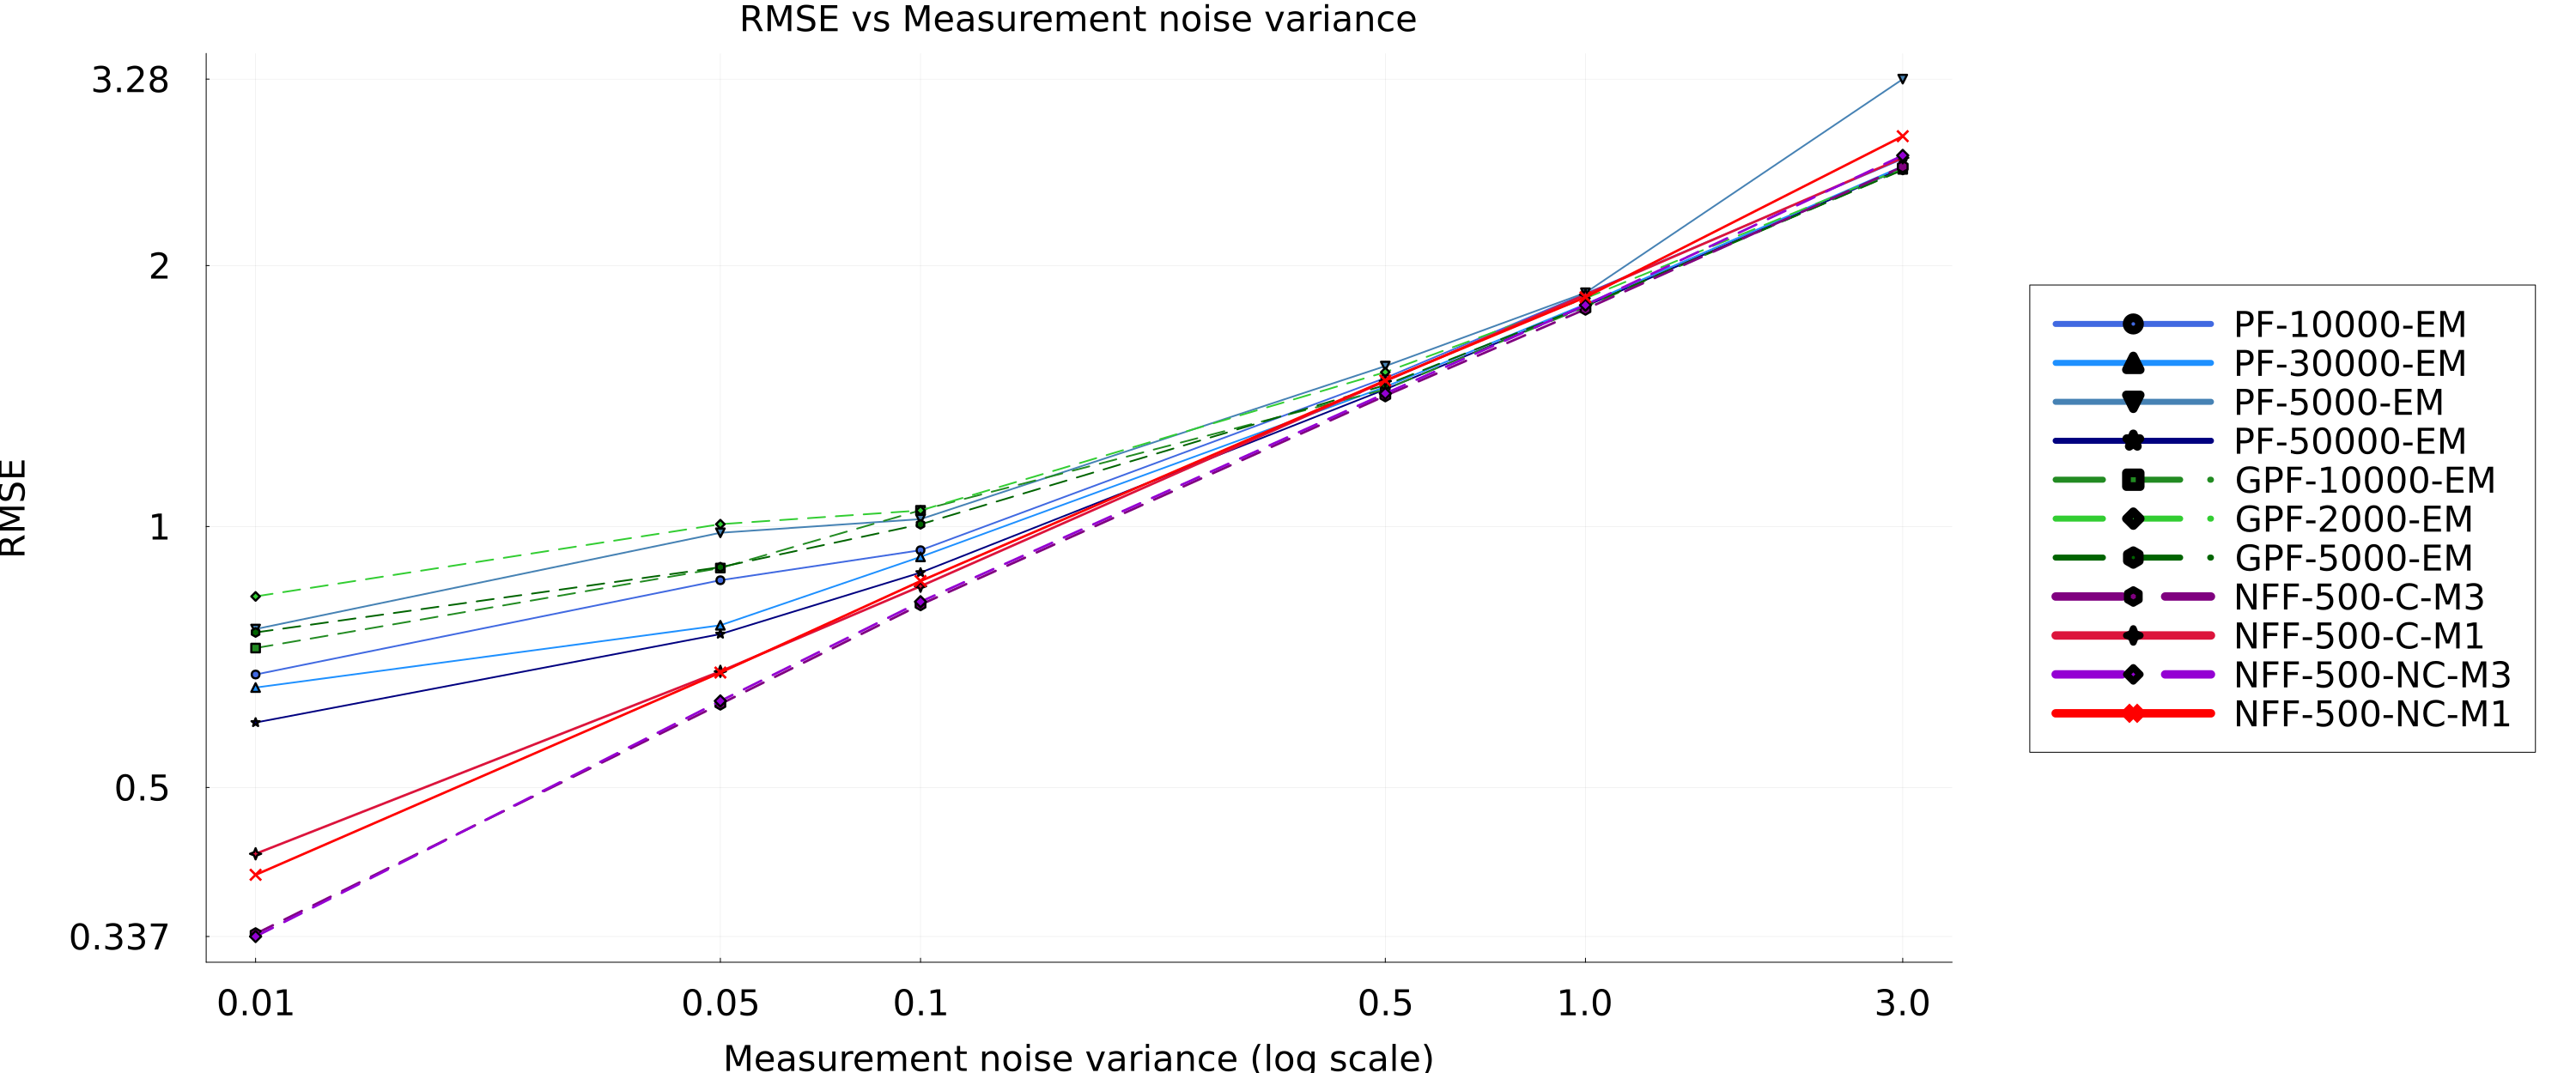
\includegraphics[width=\textwidth]{figures/Experiment06/rmse_nff_N500_vs_others_rmse.png}
		\caption{RMSE vs. measurement noise variance.}
		\label{fig:app_noise_rmse_500}
	\end{SubFigure}\hfill
	\begin{SubFigure}{0.48\textwidth}
		\centering
		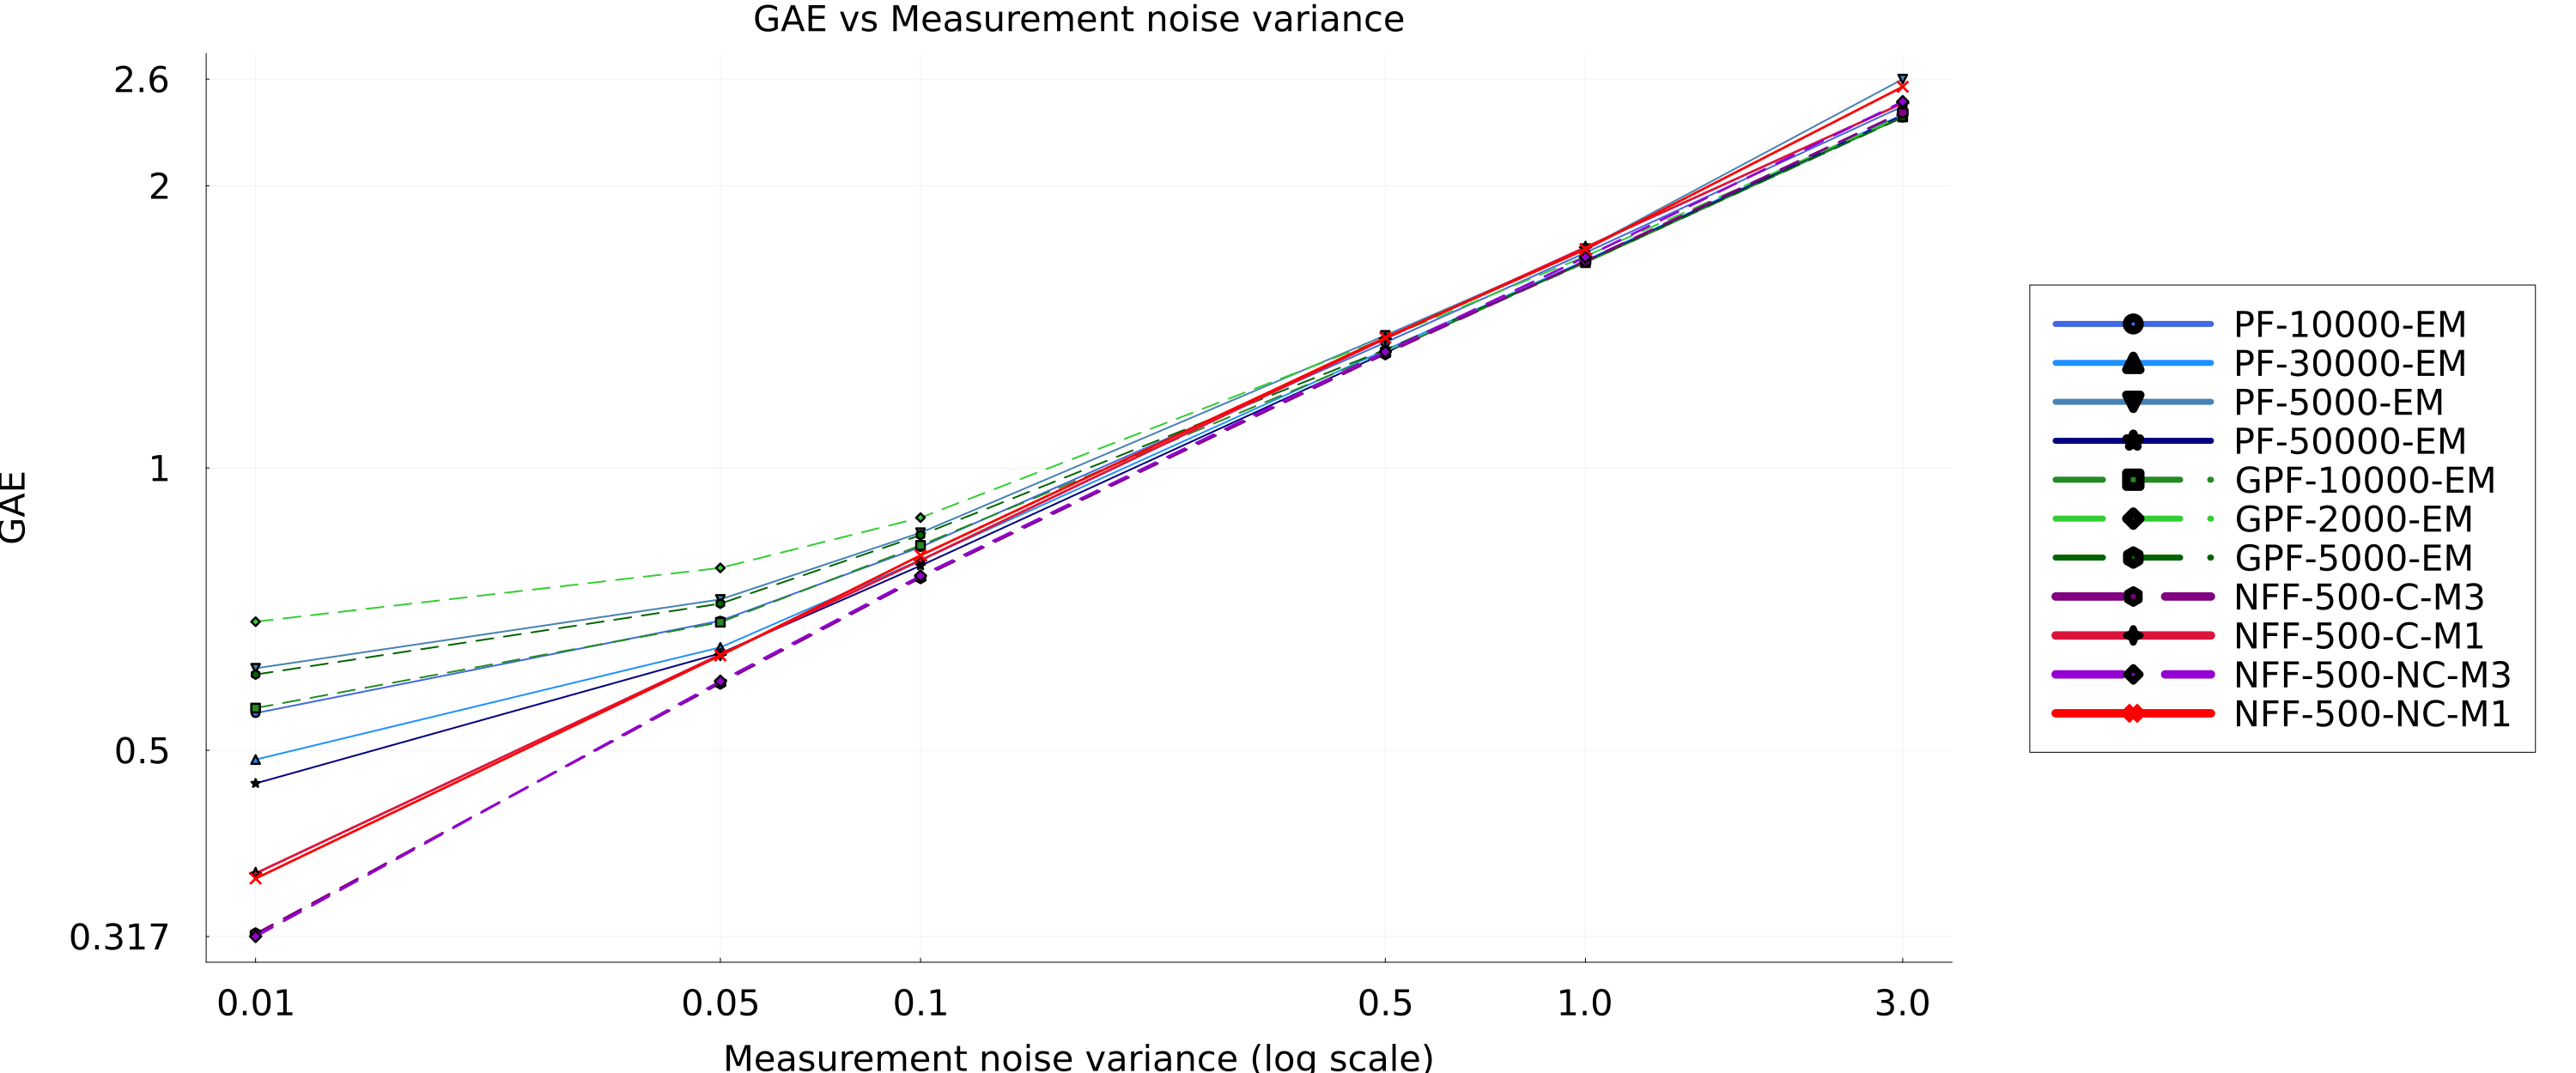
\includegraphics[width=\textwidth]{figures/Experiment06/gae_nff_N500_vs_others_gae.png}
		\caption{GAE vs. measurement noise variance.}
		\label{fig:app_noise_gae_500}
	\end{SubFigure}
	
	\vspace{0.5em}
	
	\begin{SubFigure}{0.48\textwidth}
		\centering
		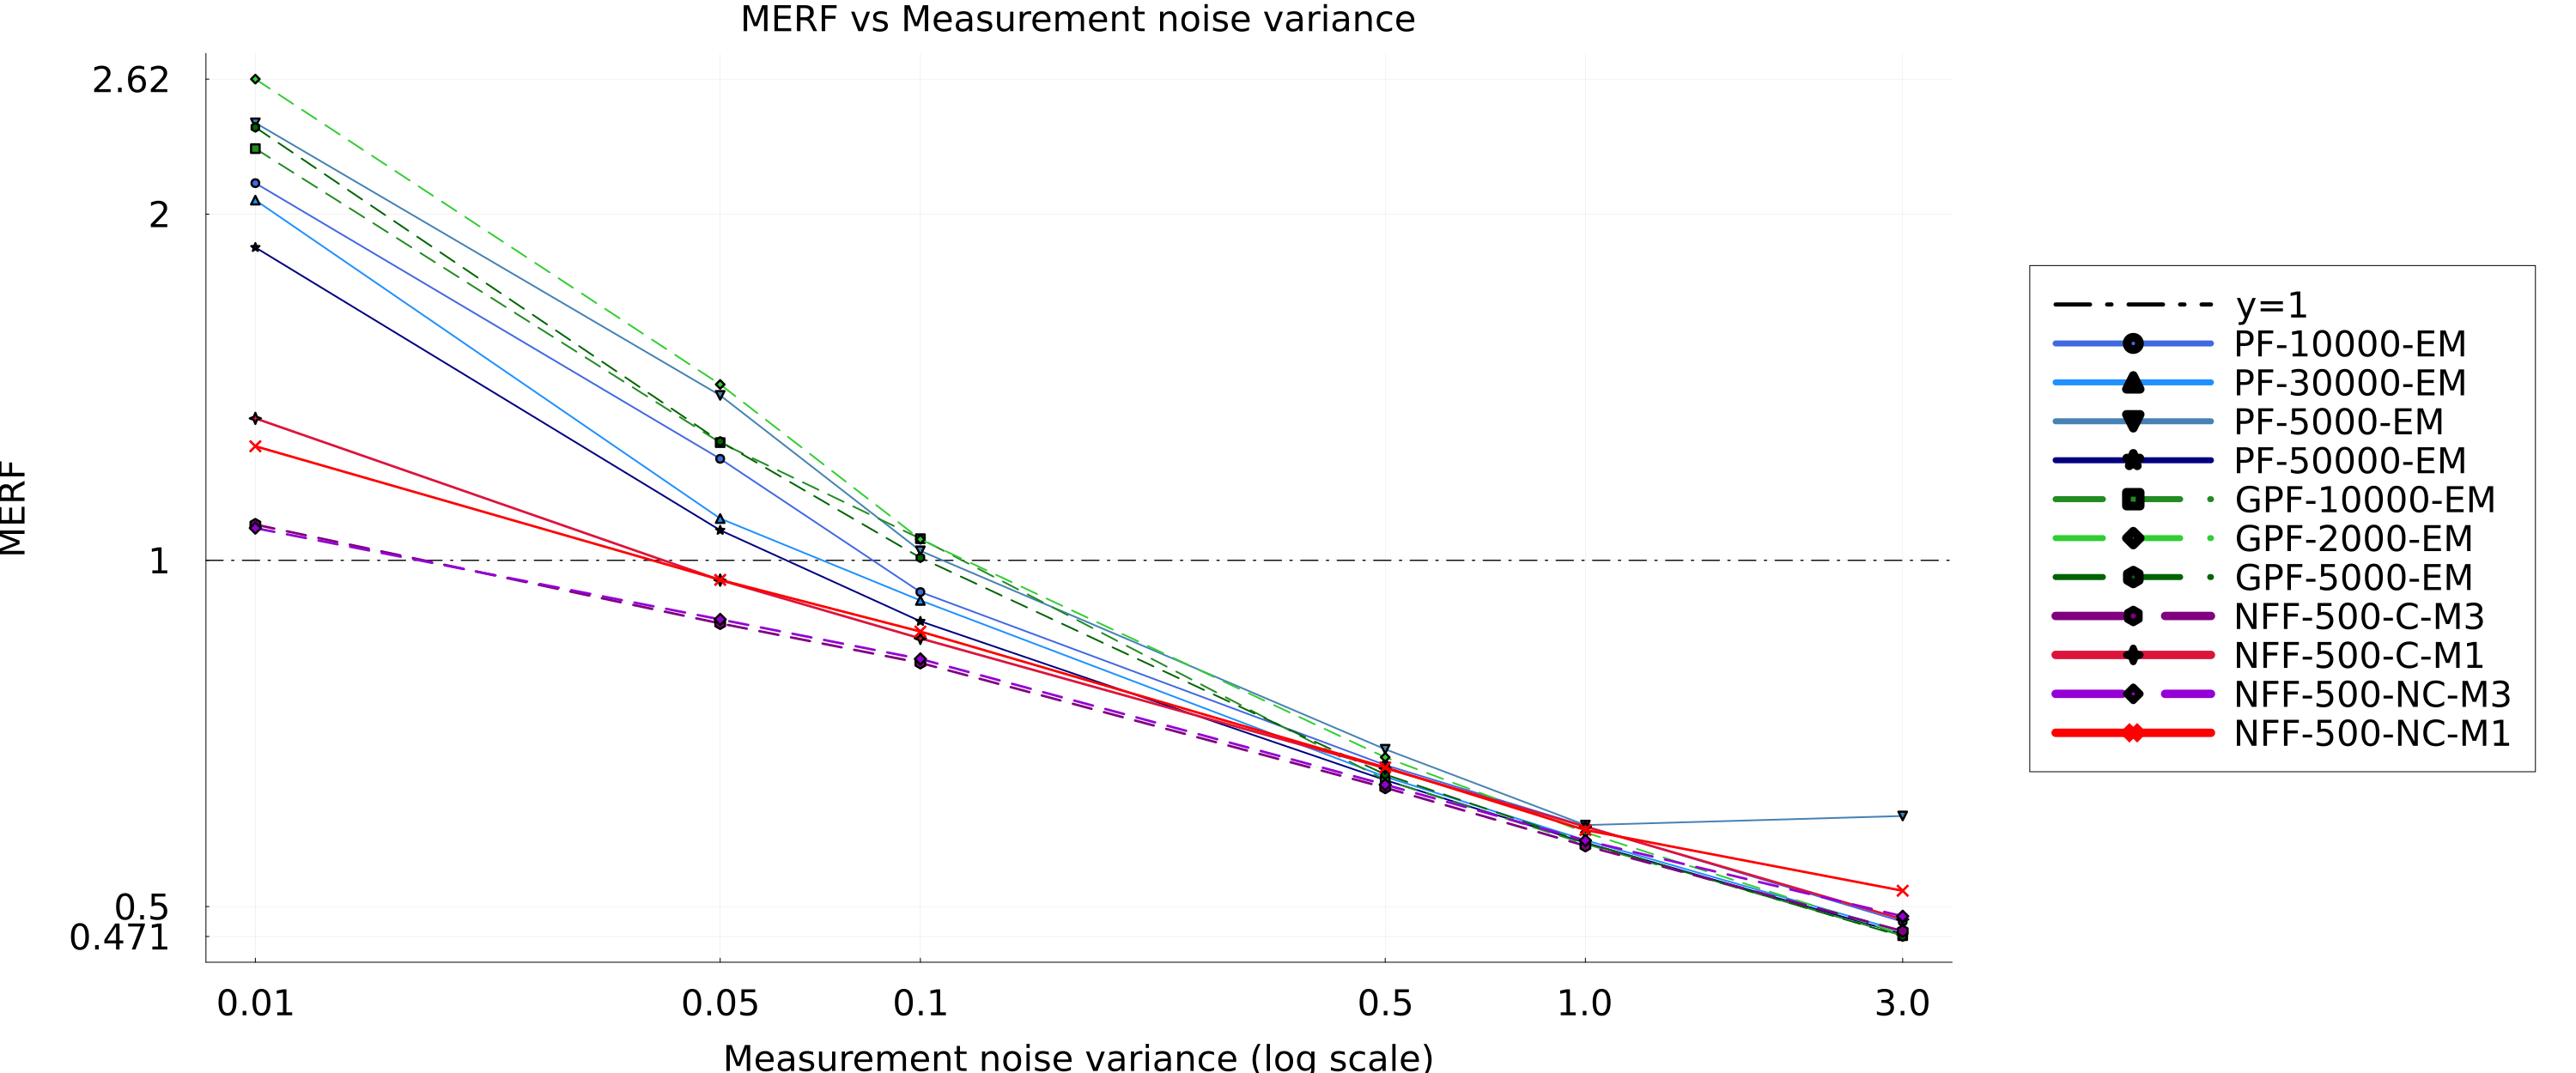
\includegraphics[width=\textwidth]{figures/Experiment06/merf_nff_N500_vs_others_merf.png}
		\caption{MERF vs. measurement noise variance.}
		\label{fig:app_noise_merf_500}
	\end{SubFigure}\hfill
	\begin{SubFigure}{0.48\textwidth}
		\centering
		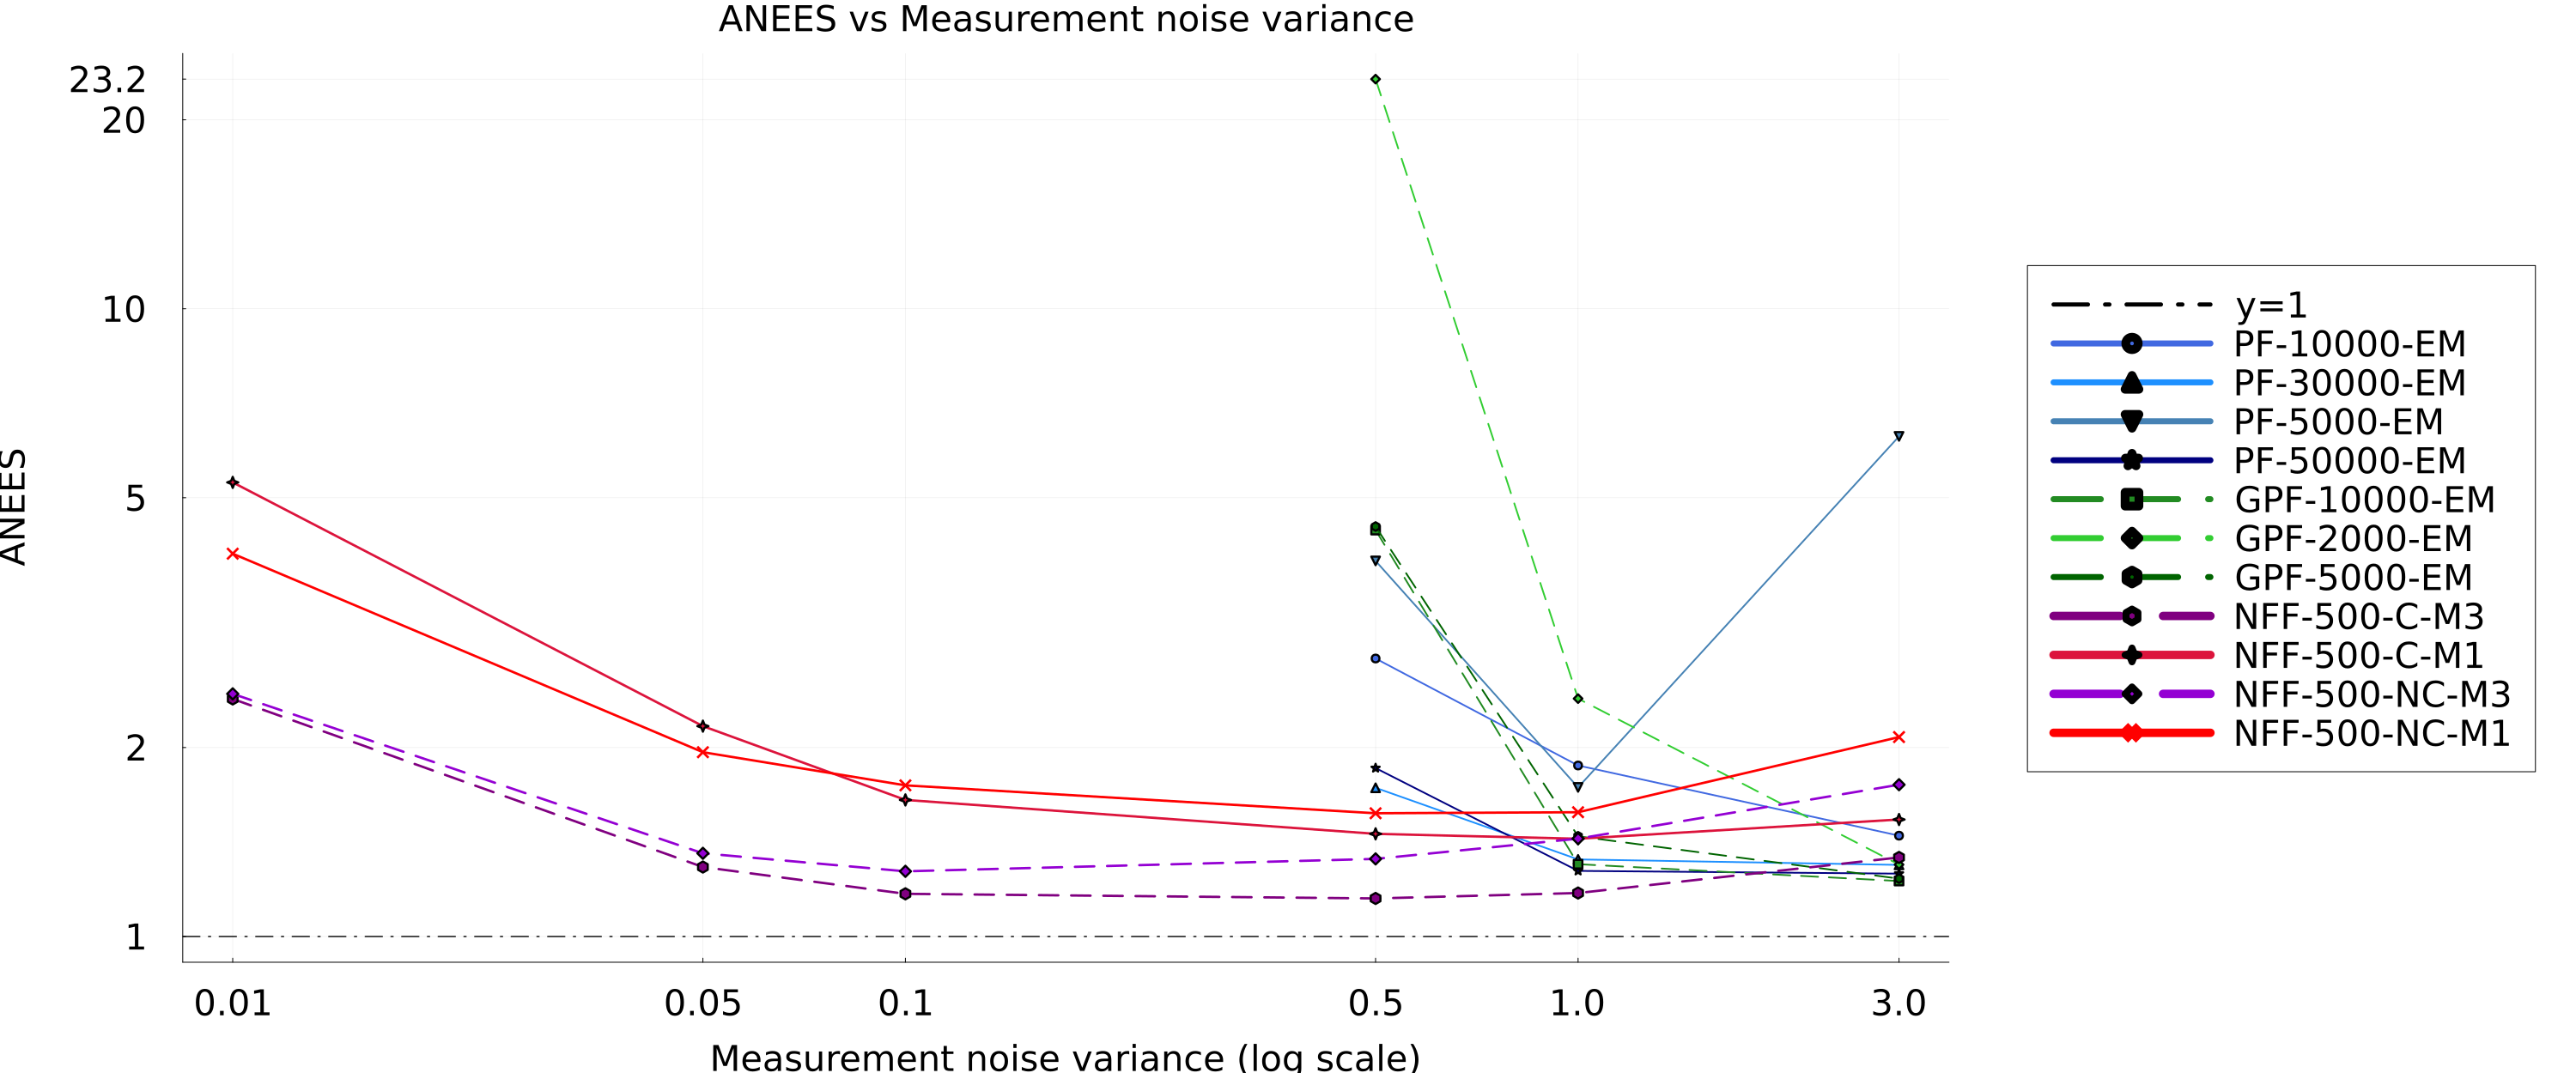
\includegraphics[width=\textwidth]{figures/Experiment06/anees_nff_N500_vs_others_anees.png}
		\caption{ANEES vs. measurement noise variance.}
		\label{fig:app_noise_anees_500}
	\end{SubFigure}
	\caption{Performance vs. measurement noise variance ($L=500$).}
	\label{fig:app_noise_500}
\end{Figure}

\begin{Figure}[ht]
	\centering
	\begin{SubFigure}{0.48\textwidth}
		\centering
		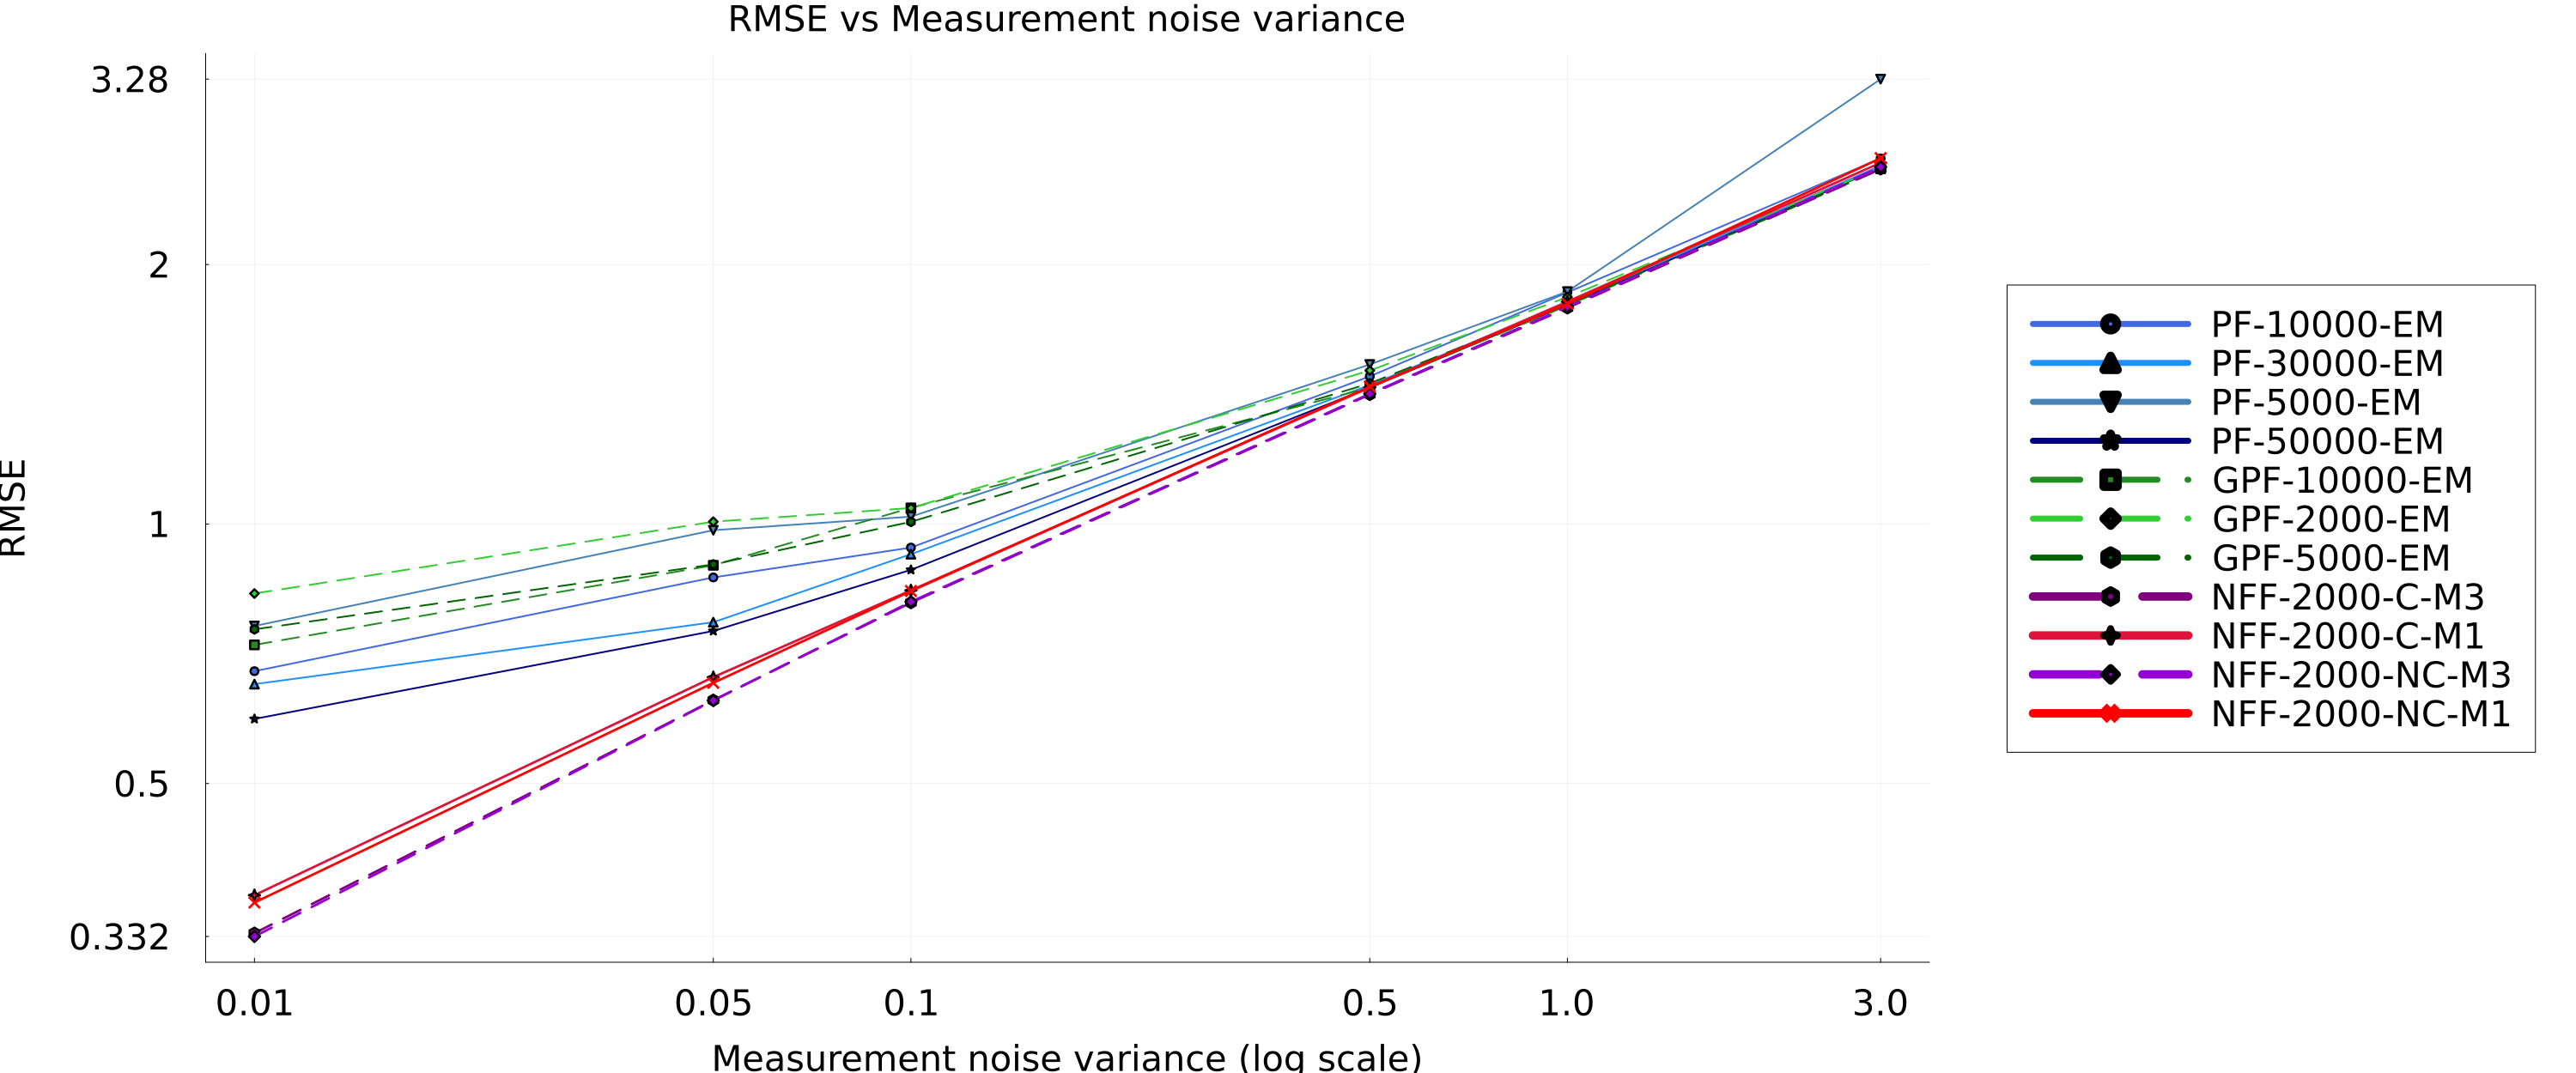
\includegraphics[width=\textwidth]{figures/Experiment06/rmse_nff_N2000_vs_others_rmse.png}
		\caption{RMSE vs. measurement noise variance.}
		\label{fig:app_noise_rmse_2000}
	\end{SubFigure}\hfill
	\begin{SubFigure}{0.48\textwidth}
		\centering
		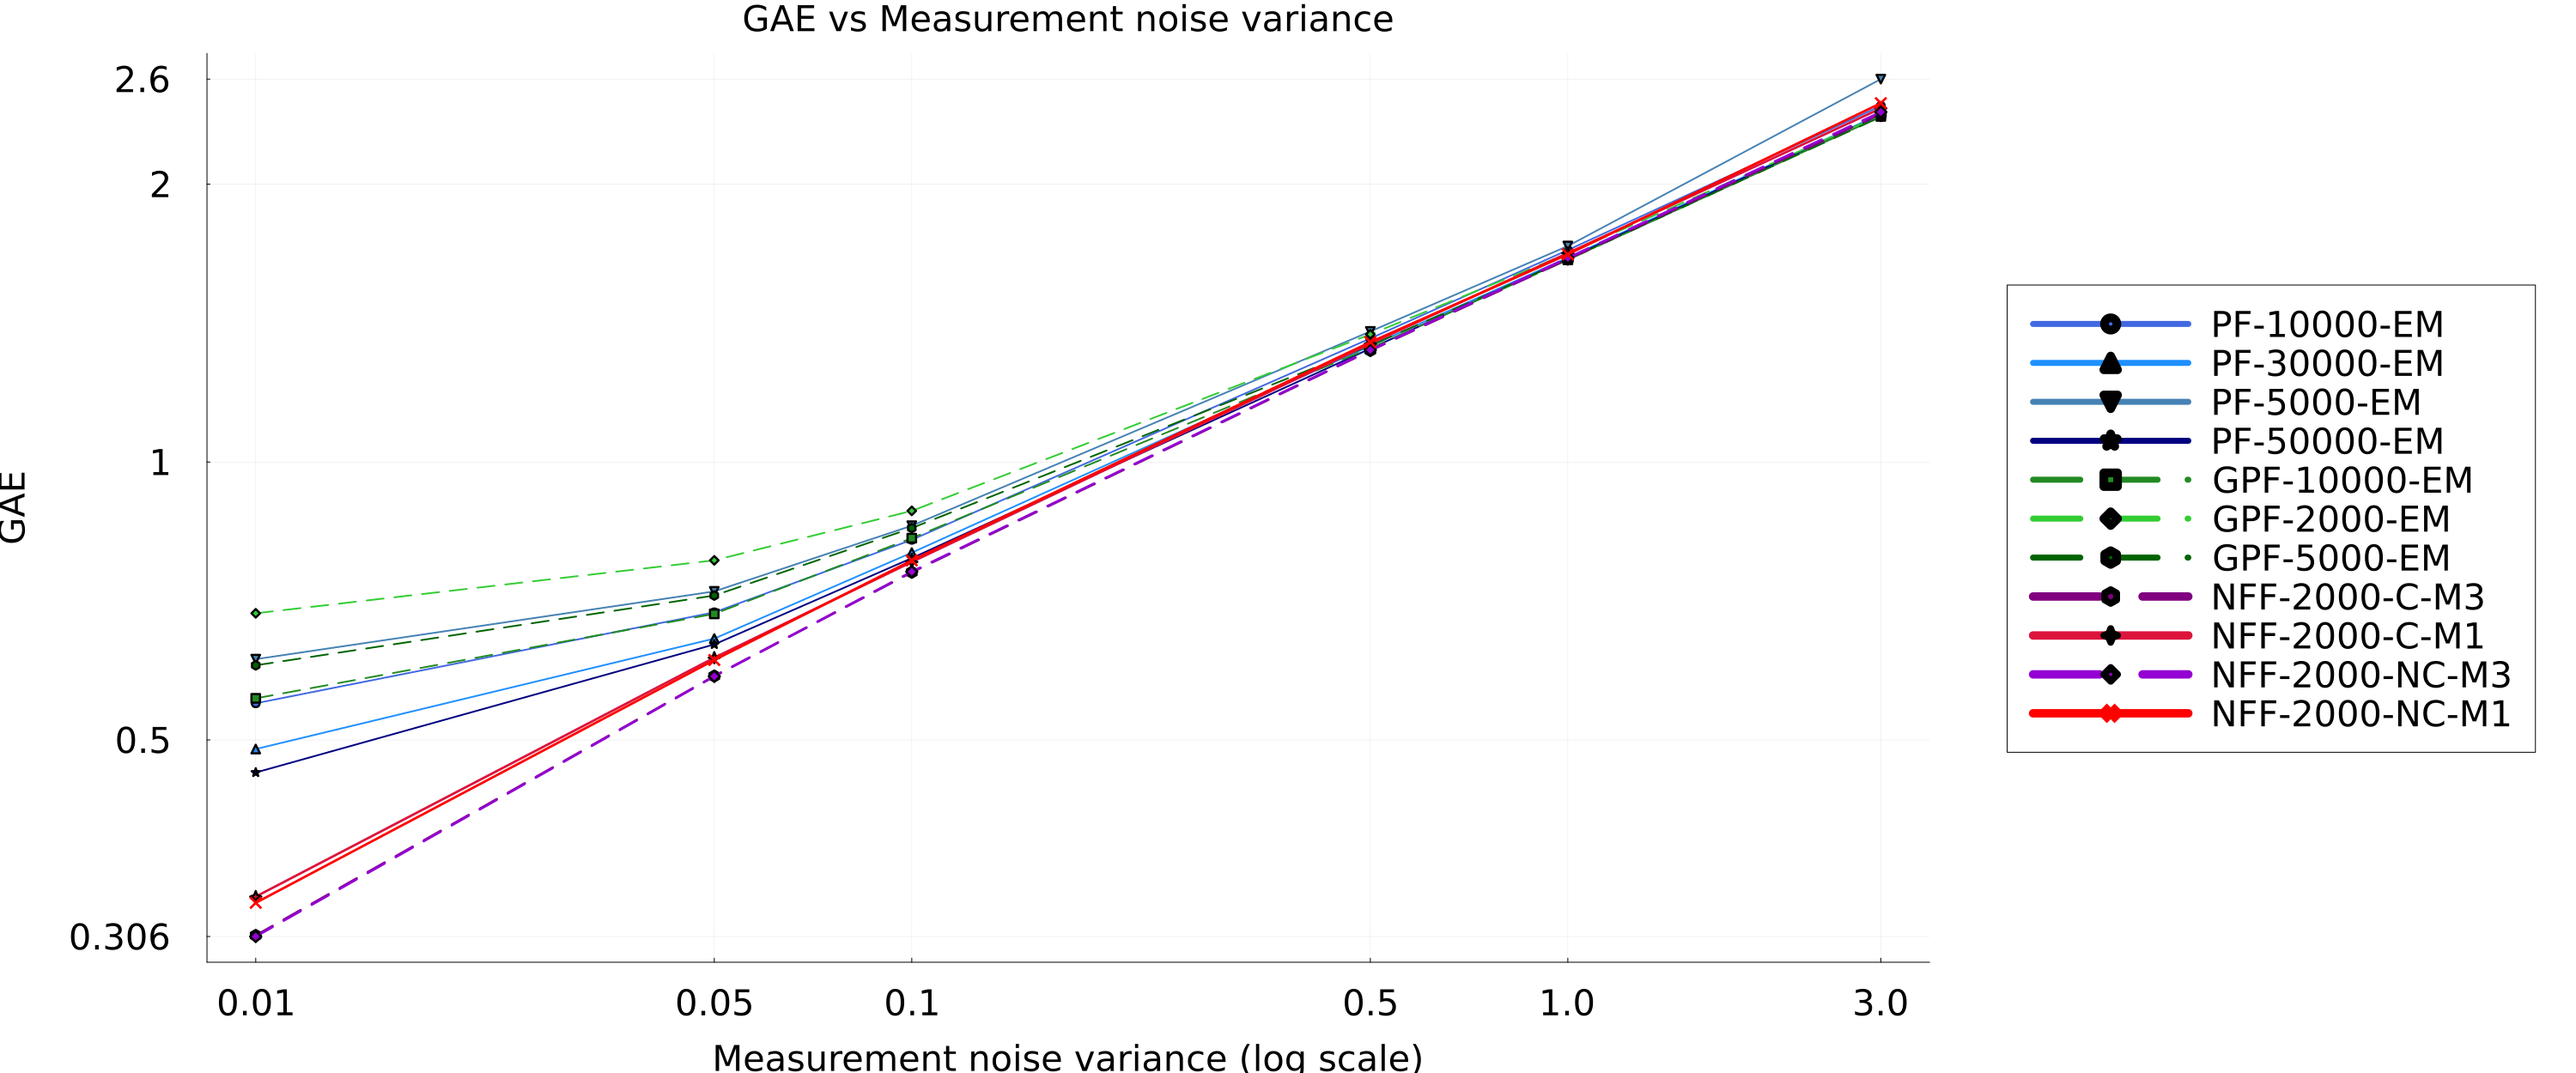
\includegraphics[width=\textwidth]{figures/Experiment06/gae_nff_N2000_vs_others_gae.png}
		\caption{GAE vs. measurement noise variance.}
		\label{fig:app_noise_gae_2000}
	\end{SubFigure}
	
	\vspace{0.5em}
	
	\begin{SubFigure}{0.48\textwidth}
		\centering
		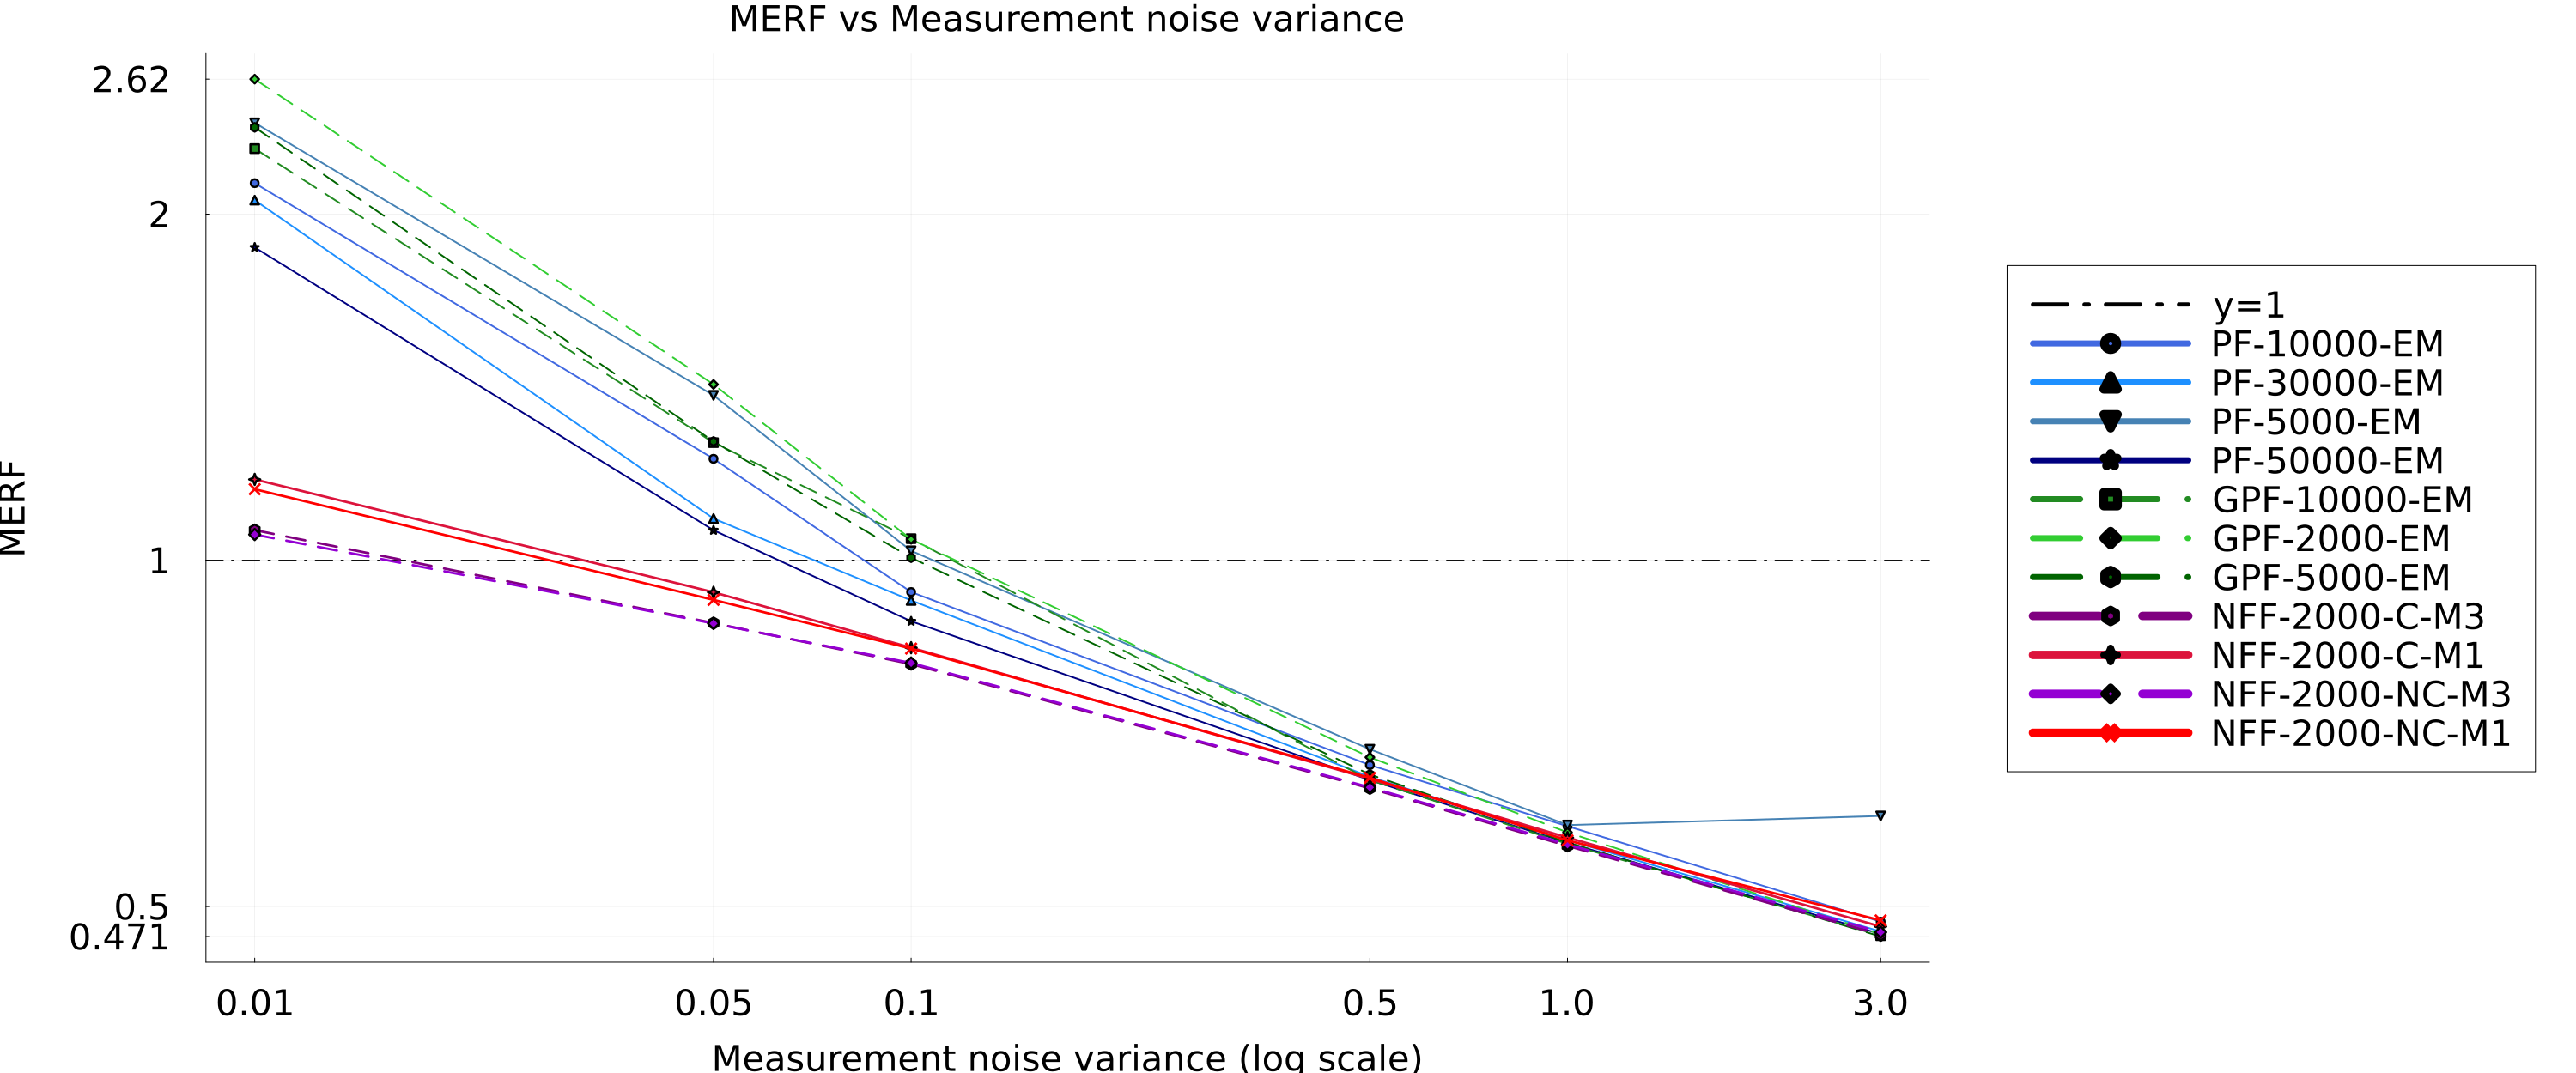
\includegraphics[width=\textwidth]{figures/Experiment06/merf_nff_N2000_vs_others_merf.png}
		\caption{MERF vs. measurement noise variance.}
		\label{fig:app_noise_merf_2000}
	\end{SubFigure}\hfill
	\begin{SubFigure}{0.48\textwidth}
		\centering
		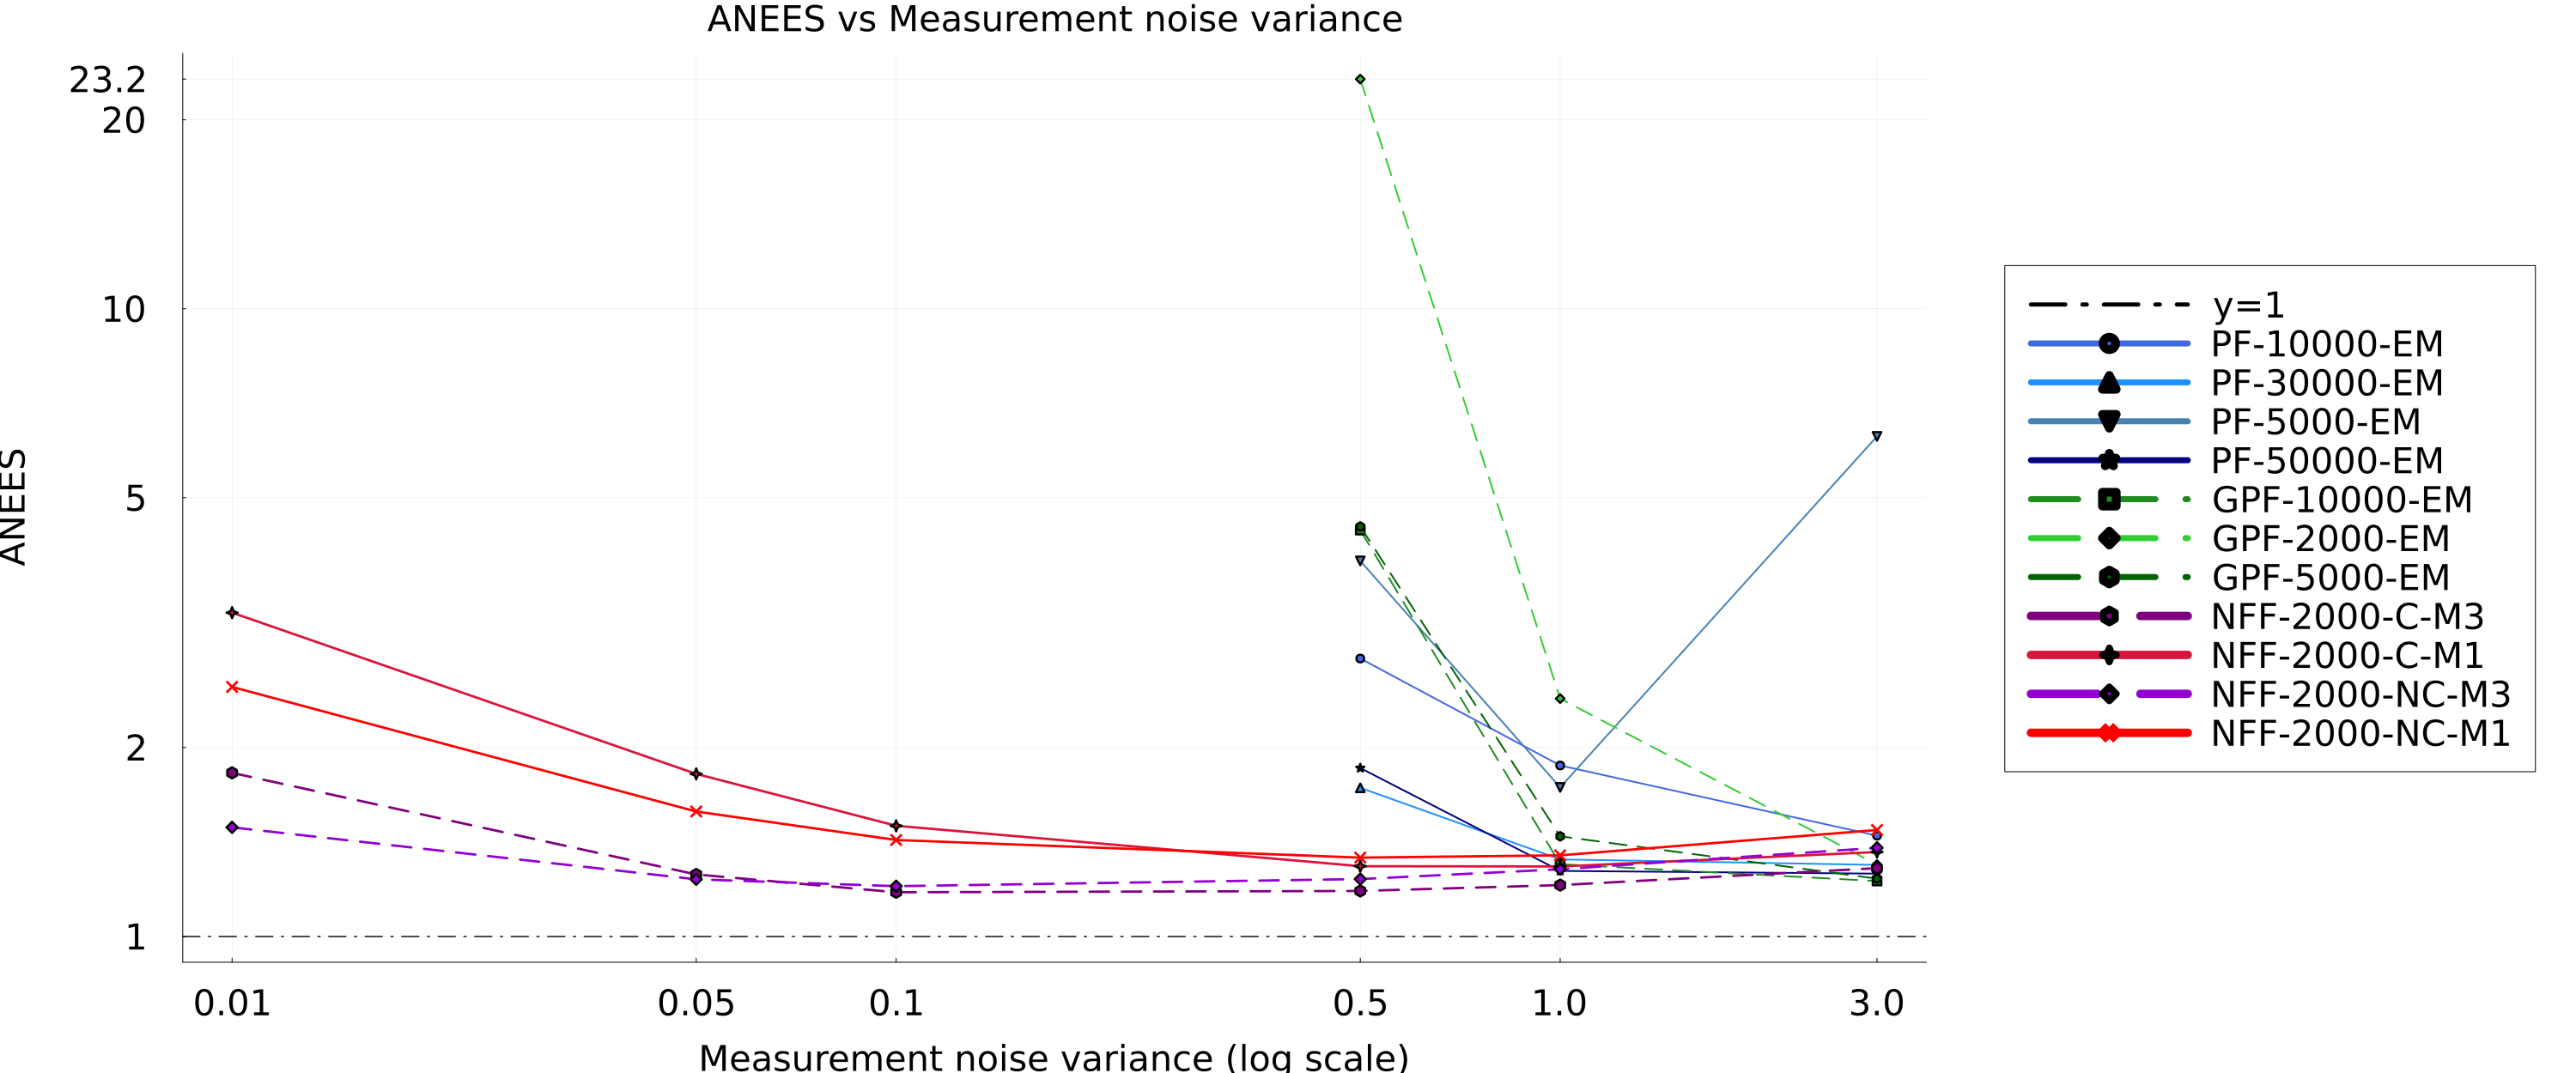
\includegraphics[width=\textwidth]{figures/Experiment06/anees_nff_N2000_vs_others_anees.png}
		\caption{ANEES vs. measurement noise variance.}
		\label{fig:app_noise_anees_2000}
	\end{SubFigure}
	\caption{Performance vs. measurement noise variance ($L=2000$).}
	\label{fig:app_noise_2000}
\end{Figure}

\clearpage

\section{Sensitivity to System Process Noise ($L=500$ and $L=2000$)}
\label{sec:app_system_noise}

\begin{Figure}[ht]
	\centering
	\begin{SubFigure}{0.48\textwidth}
		\centering
		
\includegraphics[width=\textwidth]{figures/Experiment07/rmse_nff_N500_vs_others_rmse.png}
		\caption{RMSE vs. system noise variance.}
		\label{fig:app_sysnoise_rmse_500}
	\end{SubFigure}\hfill
	\begin{SubFigure}{0.48\textwidth}
		\centering
		
\includegraphics[width=\textwidth]{figures/Experiment07/gae_nff_N500_vs_others_gae.png}
		\caption{GAE vs. system noise variance.}
		\label{fig:app_sysnoise_gae_500}
	\end{SubFigure}
	
	\vspace{0.5em}
	
	\begin{SubFigure}{0.48\textwidth}
		\centering
		
\includegraphics[width=\textwidth]{figures/Experiment07/merf_nff_N500_vs_others_merf.png}
		\caption{MERF vs. system noise variance.}
		\label{fig:app_sysnoise_merf_500}
	\end{SubFigure}\hfill
	\begin{SubFigure}{0.48\textwidth}
		\centering
		
\includegraphics[width=\textwidth]{figures/Experiment07/anees_nff_N500_vs_others_anees.png}
		\caption{ANEES vs. system noise variance.}
		\label{fig:app_sysnoise_anees_500}
	\end{SubFigure}
	\caption{Performance vs. system noise variance ($L=500$).}
	\label{fig:app_sysnoise_500}
\end{Figure}

\begin{Figure}[ht]
	\centering
	\begin{SubFigure}{0.48\textwidth}
		\centering
		
\includegraphics[width=\textwidth]{figures/Experiment07/rmse_nff_N2000_vs_others_rmse.png}
		\caption{RMSE vs. system noise variance.}
		\label{fig:app_sysnoise_rmse_2000}
	\end{SubFigure}\hfill
	\begin{SubFigure}{0.48\textwidth}
		\centering
		
\includegraphics[width=\textwidth]{figures/Experiment07/gae_nff_N2000_vs_others_gae.png}
		\caption{GAE vs. system noise variance.}
		\label{fig:app_sysnoise_gae_2000}
	\end{SubFigure}
	
	\vspace{0.5em}
	
	\begin{SubFigure}{0.48\textwidth}
		\centering
		
\includegraphics[width=\textwidth]{figures/Experiment07/merf_nff_N2000_vs_others_merf.png}
		\caption{MERF vs. system noise variance.}
		\label{fig:app_sysnoise_merf_2000}
	\end{SubFigure}\hfill
	\begin{SubFigure}{0.48\textwidth}
		\centering
		
\includegraphics[width=\textwidth]{figures/Experiment07/anees_nff_N2000_vs_others_anees.png}
		\caption{ANEES vs. system noise variance.}
		\label{fig:app_sysnoise_anees_2000}
	\end{SubFigure}
	\caption{Performance vs. system noise variance ($L=2000$).}
	\label{fig:app_sysnoise_2000}
\end{Figure}

\clearpage

\section{Sensitivity to System Nonlinearity Intensity ($L=500$ and $L=2000$)}
\label{sec:app_nonlinearity}

\begin{Figure}[ht]
	\centering
	\begin{SubFigure}{0.48\textwidth}
		\centering
		
\includegraphics[width=\textwidth]{figures/Experiment08/rmse_nff_N500_vs_others_rmse.png}
		\caption{RMSE vs. discretization time step.}
		\label{fig:app_nonlinear_rmse_500}
	\end{SubFigure}\hfill
	\begin{SubFigure}{0.48\textwidth}
		\centering
		
\includegraphics[width=\textwidth]{figures/Experiment08/gae_nff_N500_vs_others_gae.png}
		\caption{GAE vs. discretization time step.}
		\label{fig:app_nonlinear_gae_500}
	\end{SubFigure}
	
	\vspace{0.5em}
	
	\begin{SubFigure}{0.48\textwidth}
		\centering
		
\includegraphics[width=\textwidth]{figures/Experiment08/merf_nff_N500_vs_others_merf.png}
		\caption{MERF vs. discretization time step.}
		\label{fig:app_nonlinear_merf_500}
	\end{SubFigure}\hfill
	\begin{SubFigure}{0.48\textwidth}
		\centering
		
\includegraphics[width=\textwidth]{figures/Experiment08/anees_nff_N500_vs_others_anees.png}
		\caption{ANEES vs. discretization time step.}
		\label{fig:app_nonlinear_anees_500}
	\end{SubFigure}
	\caption{Performance vs. discretization time step ($L=500$).}
	\label{fig:app_nonlinear_500}
\end{Figure}

\begin{Figure}[ht]
	\centering
	\begin{SubFigure}{0.48\textwidth}
		\centering
		
\includegraphics[width=\textwidth]{figures/Experiment08/rmse_nff_N2000_vs_others_rmse.png}
		\caption{RMSE vs. discretization time step.}
		\label{fig:app_nonlinear_rmse_2000}
	\end{SubFigure}\hfill
	\begin{SubFigure}{0.48\textwidth}
		\centering
		
\includegraphics[width=\textwidth]{figures/Experiment08/gae_nff_N2000_vs_others_gae.png}
		\caption{GAE vs. discretization time step.}
		\label{fig:app_nonlinear_gae_2000}
	\end{SubFigure}
	
	\vspace{0.5em}
	
	\begin{SubFigure}{0.48\textwidth}
		\centering
		
\includegraphics[width=\textwidth]{figures/Experiment08/merf_nff_N2000_vs_others_merf.png}
		\caption{MERF vs. discretization time step.}
		\label{fig:app_nonlinear_merf_2000}
	\end{SubFigure}\hfill
	\begin{SubFigure}{0.48\textwidth}
		\centering
		
\includegraphics[width=\textwidth]{figures/Experiment08/anees_nff_N2000_vs_others_anees.png}
		\caption{ANEES vs. discretization time step.}
		\label{fig:app_nonlinear_anees_2000}
	\end{SubFigure}
	\caption{Performance vs. discretization time step ($L=2000$).}
	\label{fig:app_nonlinear_2000}
\end{Figure}

	\makebibliography{references}
	
\end{document}
